%Dokumentklasse
\documentclass[a4paper,12pt,makeidx,
twoside,
openright,
numbers=noenddot]{scrreprt}
\usepackage[left=3cm, right=2cm, bottom=2.5cm, top=3cm]{geometry}
\setlength{\headsep}{10mm}					% Abstand Kopfzeile zum Textkörper
%\usepackage[onehalfspacing]{setspace}		% verwendet für größeren Zeilenabstand

% ============= Packages =============

% Dokumentinformationen
\usepackage[
	pdftitle={Masterthesis},
	pdfsubject={},
	pdfauthor={Markus Brandt},
	pdfkeywords={},
	%Links nicht einrahmen
	hidelinks
]{hyperref}


% Standard Packages
\usepackage[utf8]{inputenc}
\usepackage[ngerman]{babel}
\usepackage[T1]{fontenc}
\usepackage{units}
\usepackage{pdfpages}
\usepackage{listings}
\usepackage{svg}					% Zur Einbindung von scalable vector graphics
\usepackage{subcaption}
\usepackage[gen]{eurosym}			% Zur Verwendung des Eurozeichens
\usepackage{amssymb}


\usepackage{graphicx}
\graphicspath{{img/}}
%\usepackage{subfigure}
\usepackage{fancyhdr}
\usepackage{color}
\usepackage{microtype} 				% schönerer Blocksatz!
\usepackage{calc}  					
\usepackage{enumitem}				% zb für align der description
\usepackage[font=small,labelfont=bf]{caption}
\usepackage[printonlyused]{acronym}	% für Abkürzungen
\usepackage{multicol}
\usepackage{booktabs}
\usepackage{textcomp}
\usepackage{listings}	% Einbindung von Code in LateX
\usepackage{setspace}
\usepackage{threeparttable} % für Fußnoten innerhalb einer Tabelle
\renewcommand{\arraystretch}{1.2}

%verschiedene Schriftarten
%\usepackage{times} 	% times font
%\usepackage{palatino} 	% Palatino font
\usepackage{lmodern}	% Lmodern sans und serif
%\usepackage{libertine}	% Linux Libertine und Biolinum

%\usepackage{fontspec}	% Nutzen in Kombination mit LuaLaTeX, um Systemschriften einzubinden
%\setmainfont{Georgia}


% zusätzliche Schriftzeichen der American Mathematical Society
\usepackage{amsfonts}
\usepackage{amsmath}

%nicht einrücken nach Absatz
\setlength{\parindent}{0pt}
\usepackage{parskip}		% verhindert einrücken und setzt einen kleinen Absatz

\usepackage[numbers, comma]{natbib}
\bibliographystyle{myabbrvnat}

\setcounter{secnumdepth}{3}		% Nummerierungsebene anpassen -> 3 = subsubsection werden nummeriert
\setcounter{tocdepth}{1}   		% gliederungsebenen im Inhaltsverzeichnis -> erstmal nur zur übersicht was nicht vergessen werden darf

\definecolor{deepblue}{rgb}{0,0,0.5}
\definecolor{deepred}{rgb}{0.6,0,0}
\definecolor{deepgreen}{rgb}{0,0.5,0}

\lstdefinestyle{Style}{
columns=flexible,
basicstyle=\ttfamily}



\lstset{ 
	backgroundcolor=\color{white},   % choose the background color; you must add \usepackage{color} or \usepackage{xcolor}; should come as last argument
	basicstyle=\footnotesize,        % the size of the fonts that are used for the code
	breakatwhitespace=false,         % sets if automatic breaks should only happen at whitespace
	breaklines=true,                 % sets automatic line breaking
	captionpos=none,                    % sets the caption-position to bottom
	commentstyle=\color{deepblue},    % comment style
	deletekeywords={...},            % if you want to delete keywords from the given language
	escapeinside={\%*}{*)},          % if you want to add LaTeX within your code
	extendedchars=true,              % lets you use non-ASCII characters; for 8-bits encodings only, does not work with UTF-8
	firstnumber=1,                % start line enumeration with line 1000
	frame=single,	                   % adds a frame around the code
	keepspaces=true,                 % keeps spaces in text, useful for keeping indentation of code (possibly needs columns=flexible)
	keywordstyle=\color{blue},       % keyword style
	language=Python,                 % the language of the code
	morekeywords={*,...},            % if you want to add more keywords to the set
	numbers=left,                    % where to put the line-numbers; possible values are (none, left, right)
	numbersep=5pt,                   % how far the line-numbers are from the code
	emphstyle=\color{deepred},
	%numberstyle=\tiny\color{mygray}, % the style that is used for the line-numbers
	rulecolor=\color{black},         % if not set, the frame-color may be changed on line-breaks within not-black text (e.g. comments (green here))
	showspaces=false,                % show spaces everywhere adding particular underscores; it overrides 'showstringspaces'
	showstringspaces=false,          % underline spaces within strings only
	showtabs=false,                  % show tabs within strings adding particular underscores
	stepnumber=2,                    % the step between two line-numbers. If it's 1, each line will be numbered
	stringstyle=\color{deepgreen},     % string literal style
	tabsize=2,	                   % sets default tabsize to 2 spaces
	title=\lstname                   % show the filename of files included with \lstinputlisting; also try caption instead of title
}


% ============= Kopf- und Fußzeile =============
\pagestyle{fancy}
%
%\lhead{\leftmark}			%slshape
%\chead{}
%\rhead{\rightmark}
% zweiseitig
\fancyhead{}
\fancyhead[RO,LE]{\thepage}
\fancyhead[RE]{\leftmark}
\fancyhead[LO]{\rightmark}
%%
\fancyfoot{}

\renewcommand{\headrulewidth}{0.4pt}
%\renewcommand{\footrulewidth}{0.4pt}				% Bei zweiseitig entfernen
\renewcommand{\chaptermark}[1]{\markboth{\thechapter\ #1}{}}
\renewcommand{\sectionmark}[1]{\markright{\thesection\ #1}}

% ============= Package Einstellungen & Sonstiges ============= 
%Besondere Trennungen
\hyphenation{Um-ge-bungs-tem-pe-ra-tur Um-ge-bungs-tem-pe-ra-tur-en Rauch-gas-tem-pe-ra-tur Aus-tritts-tem-pe-ra-tur}


% ============= Dokumentbeginn =============

\begin{document}
	
%Seiten ohne Kopf- und Fußzeile sowie Seitenzahl
\pagestyle{empty}

\begin{center}
\begin{tabular}{p{\textwidth}}

\begin{center}
	
\includegraphics[scale=0.35]{img/logos.jpg}
\end{center}


\\

\begin{center}
\LARGE{\textbf{
Untersuchung zum Einsatz von Solarthermie in
multivalenten Wärmeversorgungsnetzen\\[1cm]
}}
\end{center}

\\


\begin{center}
\large{Hochschule Flensburg\\
Fachbereich 1: \textit{Systemtechnik}\\}
\end{center}

\\\\

\begin{center}
\textbf{\Large{Abschlussarbeit}}
\end{center}


\begin{center}
zur Erlangung des akademischen Grades\\
Master of Engineering
\end{center}

\\\\

\begin{center}
vorgelegt von
\end{center}

\begin{center}
\large{\textbf{Markus Brandt}} \\
% \small{geboren am 22.10.1992 in Flensburg}
\end{center}

\begin{center}
\large{14. Oktober 2019}
\end{center}

\\
\\
\\

\begin{center}
\begin{tabular}{lll}
\textbf{Erstprüfer:} & & Prof. Dr.-Ing. Ilja Tuschy\\
\textbf{Zweitprüfer:} & &M. Eng. Francesco Witte\\
\end{tabular}
\end{center}

\end{tabular}
\end{center}
\newpage 
\thispagestyle{empty}
\quad 
\newpage
\pagenumbering{Roman}
% Beendet eine Seite und erzwingt auf den nachfolgenden Seiten die Ausgabe aller Gleitobjekte (z.B. Abbildungen), die bislang definiert, aber noch nicht ausgegeben wurden. Dieser Befehl fügt, falls nötig, eine leere Seite ein, sodaß die nächste Seite nach den Gleitobjekten eine ungerade Seitennummer hat. 
\cleardoubleoddpage


\chapter*{Eidesstattliche Erklärung}
Ich versichere, dass ich die vorliegende Thesis ohne fremde Hilfe selbstständig verfasst und nur die angegebenen Quellen benutzt habe. \\~\\
Flensburg, den 14. Oktober 2019\\[.6cm]
Markus Brandt\\
\rule[0.5em]{20em}{0.5pt}

\chapter*{Zusammenfassung}
Wärmeversorgungssysteme nachhaltig zu gestalten ist durch die Integration regenerativer Energien möglich. Mit der Solarthermie steht hierbei eine Technologie zur Verfügung, die bereits seit Jahren in Dänemark erfolgreich zur Wärmeversorgung eingesetzt wird. Das Ziel der vorliegenden Arbeit ist die Einsatzmöglichkeit solarthermischer Anlagen bezüglich ihrer Wirtschaftlichkeit in deutschen Wärmeversorgungsnetzen zu untersuchen.

Zu diesem Zweck ist ein Kraft-Wärme-Kopplung dominiertes Versorgungssystem - das Referenzsystem - um drei Konzepte der solarthermischen Wärmebereitstellung erweitert worden. Bei dem ersten Konzept handelt es sich um ein einfaches Solarthermie-Konzept, bestehend aus einem Kollektorfeld und saisonalem Wärmespeicher. Das zweite Konzept verwendet zusätzlich eine Wärmepumpe und einen Kurzzeitspeicher, um ein Wärmesystem mit erhöhtem Power-to-Heat-Anteil zu betrachten. Schließlich wird mit dem dritten System ein alternatives Konzept der solaren Wärmeerzeugung untersucht - eine Kombination aus Photovoltaik und Wärmepumpen. 

Alle Konzepte werden jeweils mit drei unterschiedlichen Kollektorflächen und Speicherkapazitäten modelliert. Die Energiesysteme werden zunächst auf Grundlage einer Einsatzoptimierung hinsichtlich ihres Kapitalwerts mit dem Referenzsystem und untereinander verglichen. Daran anschließend werden die drei wirtschaftlichsten Konzepte einer Detailanalyse unterzogen, um den Einfluss der Solarthermie auf den Betrieb des übrigen Versorgungssystems zu untersuchen. Abschließend werden Einflussanalysen durchgeführt, die den Beitrag einzelner Komponenten auf das Ergebnis der Einsatzoptimierung untersuchen.

Es zeigt sich zunächst, dass durch die Verwendung solarthermischer Anlagen der Kapitalwert des Referenzsystems gesteigert werden kann. Das einfache Solarthermie-Konzept ist hierbei aufgrund der geringen Gesamtkosten als das wirtschaftlich attraktivste Solarthermie-Konzept einzustufen. Das Photovoltaik-Konzept erreicht, trotz eines ähnlichen Erlöses, aufgrund der hohen Investitionskosten für die Wärmepumpen einen niedrigeren Kapitalwert. 

Darüber hinaus haben die Detail- und Einflussanalysen gezeigt, dass der Betrieb einer solarthermischen Anlage ohne die Verwendung eines saisonalen Wärmespeichers unwirtschaftlich ist. Ohne die Möglichkeit der Speicherung ist eine vollständige Nutzung der Solarthermie nicht erreichbar. Zusätzlich hat sich ergeben, dass das Ladeverhalten des Wärmespeichers - auch bei einer hohen Sonneneinstrahlung - bei aktuellen Randbedingungen hauptsächlich von den Strompreisen und somit vom Betrieb der Kraft-Wärme-Kopplung abhängt. Schließlich zeigt die Einflussanalyse, dass bei einem System ohne Wärmespeicher das Hinzufügen eines solchen zu der größten Kapitalwertsteigerung führt.


\tableofcontents			%Inhaltsverzeichnis
\listoffigures				%Verzeichnis aller Bilder
\listoftables				%Verzeichnis aller Tabellen
\chapter*{Abkürzungsverzeichnis}
	\begin{acronym}[PEGAS]
		\acro{4GDH}{4th Generation District Heating} 
		\acro{DH}{District Heating}
		\acro{EGIX}{European Gas Index}
		\acro{EHK}{Elektrodenheizkessel}
		\acro{GuD}{Gas- und Dampfkraftwerk}
		\acro{KWK}{Kraft-Wärme-Kopplung}
		\acro{LCOH}{Levelized Cost of Heat}
		\acro{LP}{Linear Programming}
		\acro{MILP}{Mixed-Integer Linear Programming}
		\acro{P2H}{Power to Heat}
		\acro{PEGAS}{Pan-European Gas Trading Platform}
		\acro{PR}{Performance Ratio}
		\acro{PV}{Photovoltaik}
		\acro{SF}{Solar Fraction}
		\acro{SLK}{Spitzenlastkessel}
		\acro{STES}{saisonale thermische Energiespeicher}
		\acro{STTES}{Kurzzeit thermischer Energiespeicher}
		\acro{TES}{Thermische Energiespeicher}
		\acro{TESPy}{Thermal Engineering Systems in Python}
		\acro{WP}{Wärmepumpe}
		\acro{oemof}{Open Energy Modelling Framework}
		\acro{LCOE}{Levelized Costs of Electricity}		
	\end{acronym}

\pagestyle{fancy}

\chapter{Einleitung}
\thispagestyle{empty}
\pagenumbering{arabic}

\section{Hintergrund}
Um die Energiewende bewältigen und das von der Bundesregierung angestrebte Ziel der CO$_2$-Neutralität bis zum Jahr 2050 \cite{bundesministerium2016klimaschutzplan} erreichen zu können, muss - neben der Stromversorgung - der Anteil regenerativer Energien in der Wärmeversorgung erhöht werden. Der Einsatz solarthermischer Anlagen in Nah- und Fernwärme stellt eine Möglichkeit dar, eine seit Jahren etablierte, einfache und ausgereifte Technik einzusetzen. Konzepte einer 4. Generation von Wärmenetzen betonen die Bedeutung solarthermischer Anlagen in Kombination mit saisonalen Wärmespeichern in der künftigen Wärmeversorgung \cite{LUND20141}.

Entgegen der Erwartung, dass Länder wie Italien, Portugal oder Spanien verstärkt Solarthermie einsetzen - Regionen mit einem erheblichen Dargebot an solarer Einstrahlung - ist Dänemark das weltweit führende Land im Bereich der solaren Wärmeversorgung. In Dänemark sind seit dem Jahr 1988 insgesamt 109 Solarthermie-Anlagen mit einer Größe jenseits der 1000~m² in Betrieb genommen worden. Die größte Anlage weltweit wurde 2016 in Silkeborg gebaut - die Fläche beträgt 156.694~m². Demgegenüber stehen 18 deutsche Anlagen - die Größte mit einer Fläche von 8.300~m². \cite{SDH2019} 

Der Vergleich mit Dänemark zeigt, dass die Solarthermie in einem Land mit ähnlichen Umweltbedingungen wirtschaftlich eingesetzt werden kann. Ziel dieser Arbeit ist die Untersuchung der Einsatzmöglichkeiten von Solarthermie in der norddeutschen Wärmeversorgung. Insbesondere soll untersucht werden, ob der Einsatz solarthermischer Anlagen in einem durch \ac{KWK} dominiertem Wärmesystem - in Deutschland üblich - wirtschaftlich eingesetzt werden kann. Darüber hinaus soll untersucht werden, welchen Einfluss die Solarthermie auf den Betrieb eines solchen Systems hat. 

\section{Methodik}
Um die Frage nach der Wirtschaftlichkeit solarthermischer Anlagen beantworten zu können, werden im Rahmen dieser Arbeit Modelle von Wärmeversorgungssystemen einer Einsatzoptimierung mittels linearer Programmierung unterzogen. Nach einer kurzen Zusammenfassung des aktuellen Stands der Wissenschaft, der den Leser in die Lage versetzen soll diese Arbeit in einen größeren Kontext einzuordnen, werden in dem folgenden Abschnitt zunächst die allgemein notwendigen Grundlagen zum Verständnis der Arbeit erläutert. Diese beinhalten die Definition von Wirkungsgraden, die zur Abbildung der verwendeten Technologien verwendet werden, eine Übersicht der genutzten Methoden zur wirtschaftlichen Bewertung und eine Erläuterung des eingesetzten Optimierungsverfahrens.

Aufgrund der besonderen Stellung, die Solarthermie in dieser Arbeit einnimmt, ist das daran anschließende Kapitel allein den Grundlagen der solarthermischen Wärmebereitstellung gewidmet. Es wird vor allem darauf eingegangen, wie der Ertrag solarthermischer Anlagen über die gemessene Sonneneinstrahlung bestimmt werden kann. Außerdem werden unterschiedliche Konzepte der solarthermischen Wärmebereitstellung vorgestellt, von denen drei für detaillierte Untersuchungen ausgewählt werden. Auf eine genaue Beschreibung der Funktionsweise und Besonderheiten einzelner solarthermischer Kollektoren ist verzichtet worden, da diese im Rahmen dieser Arbeit nicht relevant ist. 

Im darauf folgenden Kapitel wird die Modellierung der technischen Anlagen beschrieben. Dieser Abschnitt bespricht, welches Verhalten die verwendeten Technologien unter Teillast zeigen und wie diese entsprechend zur Einbindung in die Einsatzoptimierung zu linearisieren sind. Bei der Solarthermie wird an dieser Stelle untersucht, wie sich das Betriebsverhalten mehrerer Kollektoren von dem Verhalten eines einzelnen unterscheidet, um zu entscheiden, wie der Solarthermie-Ertrag in der Optimierung behandelt werden soll.

Bevor die Arbeit in einer Diskussion der erzielten Ergebnisse und einem Ausblick auf weiterführende Arbeiten schließt, wird in Kapitel \ref{chapter: Techno-ökonomische Betriebsmodelle} die techno-ökonomische Optimierung dargelegt. Es wird dargestellt, welche Simulationssoftware zur Optimierung eingesetzt wurde und wie die zu untersuchenden Energiesysteme in dieser Software abgebildet worden sind. Darüber hinaus werden alle Randparameter (Wetterdaten, Preiszeitreihen, etc.) besprochen, die im Rahmen dieser Arbeit verwendet wurden. Außerdem werden in diesem Kapitel für alle Energiesysteme die Ergebnisse der Optimierung dargestellt.

\section{Stand der Wissenschaft}
Im Jahr 2014 ist von \citet{LUND20141} ein Konzept für eine 4. Generation von Wärmenetzen (\ac{4GDH}) definiert worden. Darin wird hervorgehoben, dass zukünftige Wärmenetze einige Bedingungen erfüllen müssen, um nachhaltige Energiesysteme realisieren zu können. Einer von fünf genannten Kernpunkten ist die Möglichkeit erneuerbare Energien, wie beispielsweise Solar- oder Geothermie, integrieren zu können.

Aufgrund des nicht übereinstimmenden Bedarfs an Wärme und dem solaren Dargebot, welches hauptsächlich im Sommer vorliegt, ist die Verwendungen saisonaler Speicher zu empfehlen. Dies ist von \citet{CARPANETO2015714} in ihrer Arbeit über die Integration von Solarthermie in ein kleines norditalienisches Wärmenetz hervorgehoben worden.

Zunächst ist Einbringung von solarthermischer Wärme primär für relativ kleine Wärmenetze untersucht worden \cite{CARPANETO2015714, PAKERE2018549, JOLY2017865}. Eine Arbeit, die den Einsatz von Solarthermie für ein etwas größeres, aber mit maximal 16~MW Heizlast immer noch relativ kleines Wärmenetz untersucht, ist von \citet{WINTERSCHEID2017579} angefertigt worden. Hierin ist die Einbringung einer solarthermischen Anlage und eines Wärmespeichers in ein durch \ac{KWK} versorgtes Wärmenetz untersucht worden. Dies stellt in Deutschland die dominierende Art der Wärmeversorgung dar \cite{WINTERSCHEID2017579}. In einem durch das Bundesministerium für Wirtschaft und Energie geförderten Forschungsvorhaben zu Solar-\ac{KWK}-Systemen sind verschiedene Modelle unter variierenden Randbedingungen simuliert worden. Es wurde gezeigt, dass Solarthermie ohne wirtschaftliche Verluste in die Wärmeversorgung eingebracht werden kann \cite{berberich2015solar}. Gleichzeitig lässt der Bericht jedoch offen, welchen Beitrag Solar-\ac{KWK}-Systeme zukünftig in der Wärmeversorgung leisten werden.

Eine interessante Alternative zur herkömmlichen Solarthermie stellt eine Kombination aus \ac{PV} und \ac{P2H}, vorzugsweise Wärmepumpen, dar. Diese Variante der Einbringung von Sonnenenergie in die Wärmeversorgung ist jüngst von \citet{GRAVELSINS2019} untersucht worden. Sie haben gezeigt, dass in dem modellierten Energiesystem 47\% des gewonnen \ac{PV}-Stroms zum Betrieb der Wärmepumpe genutzt werden und somit die Flexibilität der \ac{PV}-Anlage vergrößert wird. Fallende \ac{PV}-Preise, die in den kommenden Jahren erwartet werden \cite{Vartiainen2019}, machen dieses Konzept für zukünftige Untersuchungen interessant.

Dieser kurze Überblick über den Stand der Wissenschaft zur Einbringung von Solarthermie in die Wärmeversorgung zeigt, dass in diesem Bereich einige Forschungsvorhaben durchgeführt wurden. Diese bezogen sich jedoch überwiegend auf relativ kleine Wärmenetze. Die Integration von Solarthermie in einem \ac{KWK} basierten System - wie sie in Deutschland typisch sind - ist in Ansätzen untersucht worden, die Wirtschaftlichkeit solcher Solar-\ac{KWK}-Systemen in einer künftigen Energieversorgung ist weiter zu untersuchen.

Diese Arbeit beschränkt sich, vor allem aufgrund der zeitlichen Begrenzung, auf die Einbringung von Solarthermie in ein größeres Wärmenetz mit einer Heizlast von maximal ca. 190~MW und untersucht, wie wirtschaftlich solche Anlagen sind. Der Aspekt der Wirtschaftlichkeit unter variierenden Randbedingungen wird nicht weiter betrachtet.

\chapter{Allgemeine Grundlagen}\label{chapter: Allgemeine Grundlagen}
\thispagestyle{empty}
\section{Bewertung verwendeter Erzeugungsanlagen}
Dieser Abschnitt stellt potentielle Technologien vor, die in einem solarthermisch gestützten Wärmeversorgungssystem zum Einsatz kommen können. Da das Ziel dieser Arbeit die Bewertung eines solchen Systems ist, wird an dieser Stelle auf eine ausführliche Beschreibung jeder einzelnen Technologie verzichtet. Die entsprechenden Unterabschnitte stellen die technologie-spezifischen Besonderheiten kurz dar und zeigen eine mögliche technische Bewertung in Form von Wirkungsgraden.
\subsection{Kraft-Wärme-Kopplung}
Unter \acf{KWK} ist die gekoppelte Erzeugung elektrischer Energie und Wärme zu verstehen. Somit stellt die \ac{KWK} eine Möglichkeit zur Sektorkopplung zwischen elektrischer Energie und Wärme dar. Im Gegensatz zu konventionellen Kraftwerken wird in Heizkraftwerken die Abwärme auf einem höheren, zu Heizzwecken nutzbaren, Temperaturniveau abgegeben. Insgesamt steigt dadurch die Brennstoffausnutzung des Kraftwerks. Um \ac{KWK}-Anlagen bewerten zu können werden folgende Kennzahlen verwendet \cite{VDI4608}:
	\begin{enumerate}
		\item Die \textbf{Heizausbeute} $\alpha$ setzt den abgegebenen Heizwärmestrom $\dot{Q}_\text{H,KWK}$ mit der zugeführten Energie ausgedrückt durch den Brennstoffmassenstrom $\dot{m}_\text{Br}$ und den Heizwert $H_\text{i}$ ins Verhältnis
		\begin{equation}\label{equation: Heizausbeute}
			\alpha = \dfrac{|\dot{Q}_\text{H,KWK}|}{\dot{m}_\text{Br}H_\text{i}}
		\end{equation}	
		
		\item Die \textbf{Stromausbeute} $\beta$ vergleicht entsprechend die abgegebene elektrische Leistung $P_\text{KWK}$ mit der zugeführten Energie
		\begin{equation}\label{equation: Stromausbeute}
			\beta = \dfrac{|P_\text{KWK}|}{\dot{m}_\text{Br}H_\text{i}}
		\end{equation}
		
		\item Der \textbf{Gesamtnutzungsfaktor} $\omega$ einer \ac{KWK}-Anlage ergibt sich nun aus der Summe der Strom- und Heizausbeute
		\begin{equation}\label{equation: Gesamtnutzungsfaktor}
			\omega = \alpha + \beta = \dfrac{|\dot{Q}_\text{H,KWK}| + |P_\text{KWK}|}{\dot{m}_\text{Br}H_\text{i}}
		\end{equation}
	\end{enumerate}
Das Betriebsverhalten von \ac{KWK}-Anlagen kann über das sogenannte PQ-Diagramm beschrieben werden, welches sich je nach verwendeter Technologie unterscheidet. Abbildung \ref{fig: PQ-Diagramm} zeigt beispielhaft die PQ-Diagramme drei unterschiedlicher Technologien. Die Schnittpunkte an der Ordinate stellen die maximal und minimal mögliche elektrische Leistung ohne Wärmeauskopplung dar. Bei der Entnahmeturbine (CCET) sorgt eine Erhöhung der ausgekoppelten Wärme zu einer Reduzierung der elektrischen Leistung, da weniger Dampf in den Endstufen der Turbine zur Verfügung steht. Dies ist beim motorischen Blockheizkraftwerk (mCHP) nicht der Fall. Bei Gegendruckturbinen (BPT) ist die elektrische Leistung fest mit der Wärmeauskopplung verbunden. Für jeden Lastpunkt kann nur eine Kombination aus elektrischer Leistung und Wärmestrom abgegeben werden. Das Gegendruckkraftwerk verfügt also über einen einzigen Freiheitsgrad. Das PQ-Diagramm reduziert sich zu einer einfachen Linie.
	\begin{figure}[htbp]
		\centering
		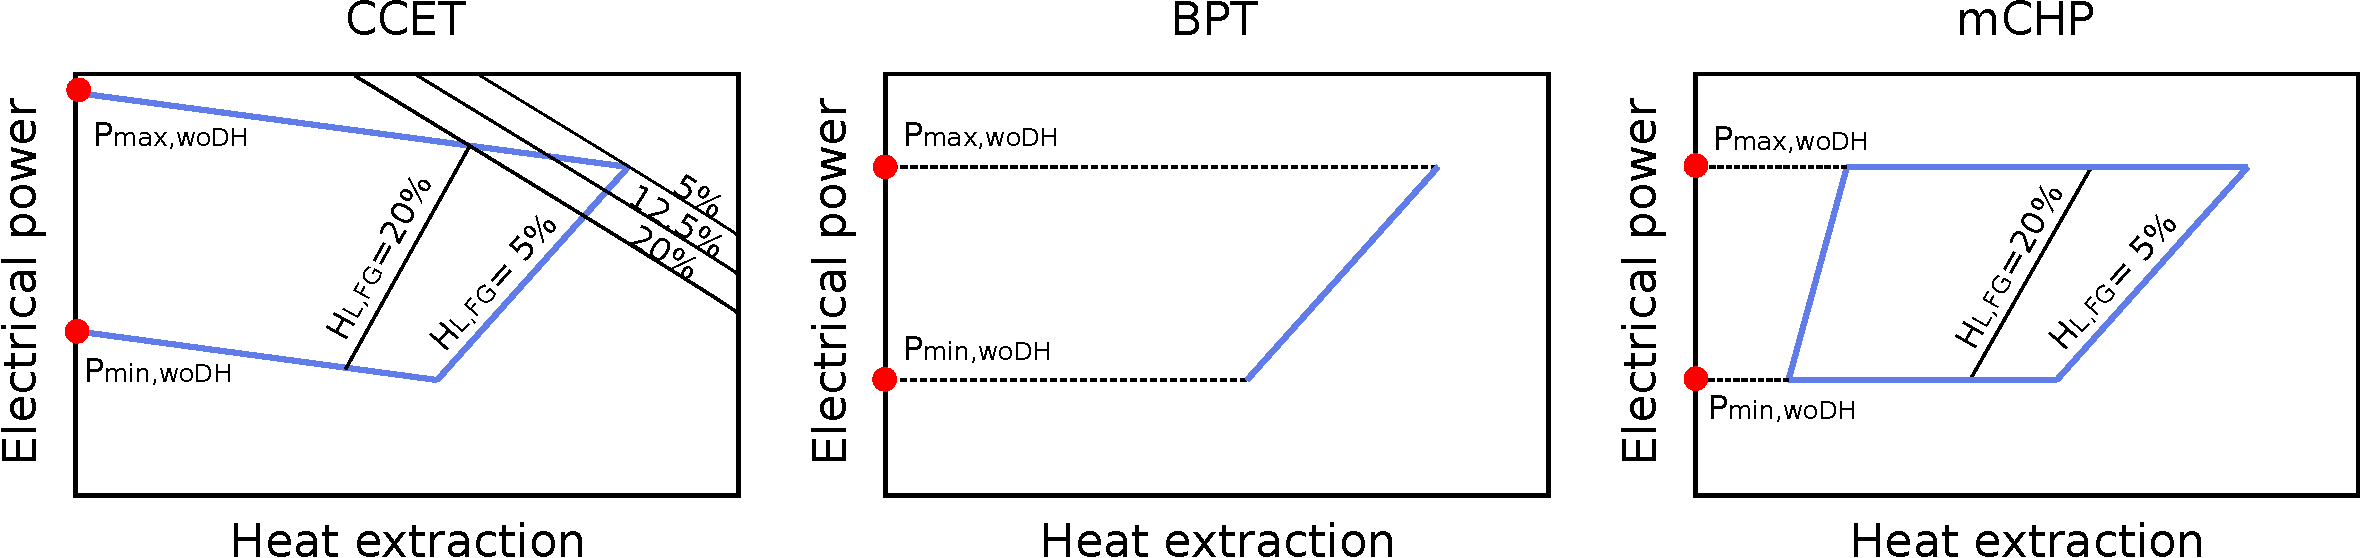
\includegraphics[width=1\linewidth]{GenericCHP.pdf}
		\captionof{figure}[Schematische Darstellung der PQ-Diagramme verschiedener KWK-Anlagen]{Schematische Darstellung der PQ-Diagramme verschiedener KWK-Anlagen. Von links: Ein \ac{GuD} mit Entnahmeschaltung (combined cycle extraction turbines - CCET), einer Gegendruckturbine (back pressure turbine - BPT) und eines motorischen Blockheizkraftwerks (motoric combined heat and power - mCHP) übernommen aus \cite{oemof2019}}
		\label{fig: PQ-Diagramm}
	\end{figure}

\subsection{Thermische Energiespeicher}

\ac{TES} bieten die Möglichkeit der zeitlichen Entkopplung der Wärmebereitstellung und des Bedarfs. Sie werden in drei verschiedenen Arten ausgeführt. Dies sind sensible Wärmespeicher, die eine fühlbare Änderung der Temperatur zur Wärmespeicherung nutzen, latent Wärmespeicher, bei denen zusätzlich die Energie des Phasenwechsels genutzt wird und schließlich thermochemische Wärmespeicher, die chemische Reaktionen zur Wärmespeicherung verwenden. Am besten erforscht und am kostengünstigsten sind die sensiblen Wärmespeicher, weshalb diese Speicher in der Wärmeversorgung vorzugsweise eingesetzt werden. \cite{Sterner2017}

Es gibt zwei mögliche Einsatzzwecke:
	\begin{description}[leftmargin=!,labelwidth=\widthof{\bfseries Saisonale Wärmespeicher}]
		\item[Saisonale Wärmespeicher] Speicherung thermischer Energie über mehrere Monate
		\item[Kurzzeitspeicher] Speicherung thermischer Energie über mehrere Stunden oder Tage.
	\end{description}
Bei solarthermisch gestützten Wärmeversorgungsnetzen wird ein \ac{STES} im Sommer geladen, da das Angebot von Solarenergie zu dieser Zeit besonders hoch ist. Im Winter wird diese Energie genutzt, wodurch sich die \ac{SF} des Systems erhöht. Kurzzeitspeicher können in Kombination mit \ac{P2H} hingegen kurzzeitige Strompreisschwankungen ausnutzen.

Zur Bewertung thermischer Energiespeicher wird der Speicherwirkungsgrad $\eta_\text{sp}$ verwendet, der sich aus dem Quotienten der abgegebenen Wärme $Q_\text{ab,sp}$ und der zugeführten Wärme $Q_\text{zu,sp}$ bildet.
	\begin{equation}\label{equation: Speicherwirkungsgrad}
		\eta_\text{sp} = \dfrac{Q_\text{ab,sp}}{Q_\text{zu,sp}}
	\end{equation} 
Die Kapazität eines sensiblen Wärmespeichers hängt von der Gesamtmasse des Speichermediums $m$, der spezifischen Wärmekapazität $c_\text{p}$ und der Temperaturdifferenz $\Delta T$ zwischen maximaler und minimaler Temperatur ab:
	\begin{equation}\label{equation: Speicherkapazität}
		Q_\text{sp} = m \cdot c_\text{p} \cdot \Delta T
	\end{equation} 
Nach \citet{CARPANETO2015714} wird der Einsatz solarthermischer Anlagen wirtschaftlich erst interessant, wenn saisonale Wärmespeicher eingesetzt werden.

\subsection{Elektrodenheizkessel}
Der \acf{EHK} ist eine mögliche Art der \ac{P2H}. Elektrische Energie wird direkt in Wärme umgesetzt, was theoretisch vollständig möglich ist. Zur Bewertung einer \ac{P2H}-Anlage, wie dem Elektrodenheizkessel oder der Wärmepumpe aus Kapitel \ref{subsection: Wärmepumpe}, ist die Definition der Systemgrenzen entscheidend, da die benötigte elektrische Energie aus einer anderen Quelle bezogen wird, welche ihrerseits Primärenergie mit einem entsprechenden Wirkungsgrad umwandelt. \citet{Baehr2012} haben den Wirkungsgrad entsprechend genau formuliert. Sofern die Systemgrenze jedoch ausschließlich um die entsprechende Anlage gezogen wird, kann der Wirkungsgrad über das Verhältnis der zugeführten elektrischen Leistung $P_\text{zu,ehk}$ und dem abgegebenen Wärmestrom $\dot{Q}_\text{ab,ehk}$ beschrieben werden. Dies wird in Gleichung \ref{equation: Elektrodenheizkessel Wirkungsgrad} dargestellt.
	\begin{equation}\label{equation: Elektrodenheizkessel Wirkungsgrad}
		\eta_\text{ehk} = \frac{|\dot{Q}_\text{ab,ehk}|}{P_\text{zu,ehk}}
	\end{equation}
Diese Beschreibung ist im Rahmen dieser Arbeit als ausreichend anzusehen.

\subsection{Spitzenlastkessel}
\acf{SLK} werden typischer Weise eingesetzt, um Bedarfsspitzen in der Wärmeversorgung zu decken. Der verwendete Brennstoff wird ausschließlich zur Wärmebereitstellung genutzt. Der Wirkungsgrad des \ac{SLK} bildet sich aus dem Quotienten des abgegebenen Wärmestroms und dem zugeführten Brennstoffmassenstrom und dem entsprechenden Heizwert. Dies wird in Gleichung \ref{equation: SLK Eta} veranschaulicht.
	\begin{equation}
		\label{equation: SLK Eta}
		\eta_\text{slk} = 	\frac{|\dot{Q}_\text{ab,slk}|}{\dot{m}_\text{Br} H_\text{i}}	
	\end{equation}

\subsection{Kompressionswärmepumpe}\label{subsection: Wärmepumpe}
Allgemein können Wärmepumpen in drei Kategorien eingeteilt werden - die sich stark voneinander unterschieden. Auf Absorptions- und Adsorptionswärmepumpen wird in dieser Arbeit jedoch nicht weiter eingegangen, da Kompressionswärmepumpen die Möglichkeit bieten, elektrische Energie zur Wärmebereitstellung zu nutzen und somit zur Sektorkopplung zwischen der Wärme- und Stromversorgung beitragen. 

Die Effizienz einer Wärmepumpe kann nicht, wie bei anderen Technologien, über einen gewöhnlichen Wirkungsgrad beschrieben werden. Im Fall der Wärmepumpe würde die herkömmliche Beschreibung des Wirkungsgrads zu einem Wert über 100\% führen, was aus Sicht der Thermodynamik als unsinnig zu bewerten ist. Aus diesem Grund ist die sogenannte Leistungszahl $\varepsilon_\text{WP}$ zur Bewertung von Wärmepumpen eingeführt worden. Diese ist in Gleichung \ref{equation: Leistungszahl 1} dargestellt und bildet sich über den abgegebenen Wärmestrom $\dot{Q}_\text{WP,ab}$ und die hinzugefügte elektrische Leistung $P_\text{WP}$ \cite{Baehr2012}.
	\begin{equation}\label{equation: Leistungszahl 1}
		\varepsilon_\text{WP} = \dfrac{|\dot{Q}_\text{WP,ab}|}{P_\text{WP}}
	\end{equation}
Über den Gütegrad $\eta_\text{WP}$ der Wärmepumpe und die Carnot-Leistungszahl $\varepsilon_\text{WPC}$ lässt sich die Leistungszahl in Abhängigkeit der Temperatur der Wärmezufuhr $T_\text{zu}$ und Wärmeabfuhr $T_\text{ab}$ darstellen \cite{HESARAKI20151199}. Dies ist entsprechend in Gleichung \ref{equation: Leistungszahl 2} dargestellt.
	\begin{equation}\label{equation: Leistungszahl 2}
		\varepsilon_\text{WP} = \varepsilon_\text{WPC} \cdot \eta_\text{WP} = \dfrac{T_\text{ab}}{T_\text{ab} - T_\text{zu}} \cdot \eta_\text{WP}
	\end{equation}


\subsection{Photovoltaik}\label{subsection: Grundlagen Photovoltaik}
Unter \ac{PV} ist die direkte Umwandlung von Sonnenstrahlung in elektrischen Strom zu verstehen. Der von \ac{PV}-Modulen bereitgestellte Gleichstrom wird über Wechselrichter in Wechselstrom umgewandelt und dem elektrischen Netz zugeführt \cite{Watter2013}. Die Photovoltaik kann in Kombination mit \ac{P2H} ebenfalls als eine Form der Solarthermie betrachtet werden, da der gewonnene elektrische Strom umgehend in Wärme umgewandelt werden kann. Ein Vorteil dieser Art der Wärmebereitstellung ist die Tatsache, dass es möglich ist sich je nach Bedarf und Kostensituation gegen die Umwandlung in Wärme zu entscheiden und den Strom direkt zu vermarkten.

Aufgrund der Tatsache, dass der \ac{PV}-Wirkungsgrad von  vielen Faktoren, wie der Einstrahlung, Umgebungstemperatur und den Windverhältnissen abhängt, wird zum Vergleich netzgekoppelter \ac{PV}-Anlagen häufig der sogenannte \ac{PR} verwendet. Dieser gibt das Verhältnis des realen Modulertrags $E_\text{PV,real}$ und des Ertrags bei Modul-Nennwirkungsgrad unter idealen Bedingungen an $E_\text{PV,ideal}$ - dargestellt in Gleichung \ref{equation: Performance Ratio}. In Deutschland liegt der \ac{PR} typischerweise zwischen 80 und 90\%. \cite{ISE}
	\begin{equation}\label{equation: Performance Ratio}
		\text{\textit{PR}} = \dfrac{E_\text{PV,real}}{E_\text{PV,ideal}}
	\end{equation}

Die elektrische Leistung $P_\text{PV}$ eines \ac{PV}-Moduls kann über Gleichung \ref{equation: LeistungPV} beschrieben werden, in der die Einstrahlung auf die geneigte Ebene $E_\text{G,gen}$ (vgl. Kapitel \ref{Funktionsweise Solarthermische Wärmebereitstellung}) mit dem Performance Ratio $\text{\textit{PR}}$, dem Modulwirkungsgrad $\eta_\text{PV}$ und Wechselrichterswirkungsgrad $\eta_\text{WR}$ multipliziert wird.
	\begin{equation}\label{equation: LeistungPV}
		P_\text{PV} = E_\text{G,gen} \cdot \text{\textit{PR}} \cdot \eta_\text{PV} \cdot \eta_\text{WR}
	\end{equation}


\section{Wirtschaftliche Bewertung}\label{section: Wirtschaftliche Bewertung}
Dieser Abschnitt wird die verwendeten Ansätze zur wirtschaftlichen Bewertung der Energiesysteme besprechen. Dabei wird zunächst die Kapitalwertmethode vorgestellt, die genutzt worden ist, um die Systeme untereinander zu vergleichen - anschließend wird vorgestellt, wie die Wärmegestehungskosten berechnet werden. Abschließen wird dieser Abschnitt mit einer Beschreibung der verwendeten Kostendegression bei variierender Anlagendimensionierungen.

\subsection{Investitionsrechnung nach Kapitalwertmethode}\label{subsection: Methoden der Investitionsrechnung}
Für Unternehmen gibt es verschiedene Investitionsmöglichkeiten. Dies können beispielsweise Investitionen in technische Anlagen, Gebäude oder Projekte sein. Darüber hinaus verfolgt jede Investition das Ziel der langfristigen Gewinnmaximierung. Oft stehen mehrere Optionen für eine Investition gleichzeitig zur Verfügung. Dies können bei technischen Anlagen beispielsweise verschiedene Konzepte oder Angebote verschiedener Hersteller sein. 

Es ist die Aufgabe der Investitionsrechnung, alle Optionen finanzmathematisch zu vergleichen und eine Aussage darüber zu treffen, welche Investition die wirtschaftlich günstigste ist. Hierzu stehen verschiedene Verfahren zur Verfügung, die der Vollständigkeit halber in folgender Übersicht zusammengestellt sind \cite{Boesch2013}. Anschließend werden kurz die entsprechenden Vor- und Nachteile besprochen, um die Methodenwahl dieser Arbeit zu begründen:
	\begin{enumerate}
		\item statische Verfahren
			\begin{itemize}
				\item Kostenvergleichsrechnung
				\item Gewinnvergleichsrechnung
				\item Amortisationsvergleichsrechnung
			\end{itemize}
		\item dynamische Verfahren
			\begin{itemize}
				\item Kapitalwertmethode
				\item interne Zinssatzmethode 
				\item Annuitätenmethode
			\end{itemize}
	\end{enumerate}
Bei statischen Verfahren werden die Zahlungen, im Gegensatz zu den dynamischen Verfahren, nicht diskontiert, weshalb sie für Investitionen mit langen Laufzeiten ungeeignet sind. Die Kapitalwertmethode ist die grundlegende und einfachste Methode der dynamischen Verfahren. Sie ist jedoch nicht auf Investitionen mit unterschiedlichen Laufzeiten anwendbar. Die Annuitätenmethode ist entsprechend komplexer, ist jedoch für Investitionen mit unterschiedlicher Laufzeit geeignet. Die interne Zinssatzmethode ist nicht auf Kosteninvestitionen anwendbar. \cite{Boesch2013}
  
Aufgrund ihrer Einfachheit und der Tatsache, dass allen untersuchten Konzepten und technischen Optionen im Rahmen dieser Arbeit die selbe Laufzeit unterstellt wird, ist die Kapitalwertmethode verwendet worden. Bei diesem Verfahren wird der Kapitalwert einer Investition zum Zeitpunkt der Inbetriebnahme $K_0$ bestimmt, in dem die Summe der Barwerte aller Einnahmen $E_t$ und Ausgaben $A_t$ des jeweiligen Jahres mit der Investitionsausgabe $I_0$ verrechnet werden. Nach \citet{Konstantin2013} kann der Kapitalwert einer Investition über Gleichung \ref{equation: Kapitalwertmethode} bestimmt werden.
	\begin{equation}\label{equation: Kapitalwertmethode}
		K_0 = -I_0 + \sum \limits_{t=1}^{t=n}\dfrac{E_t - A_t}{q^t}  
	\end{equation}
Sofern der Einnahmeüberschuss konstant ist, vereinfacht sich Gleichung \ref{equation: Kapitalwertmethode} zu:
	\begin{equation}
		\label{equation: Kapitalwert-vereinfact}
		K_0 = -I_0 + (E - A) \cdot \dfrac{q^n - 1}{q^n (q - 1)} 
	\end{equation}
hierin ist:
	\begin{tabbing}
		\hspace{0.5cm}\=\hspace{0.5cm}\=\hspace{0.5cm}\=\hspace{1cm}\=\kill
		\> $K_0$ \>: \> Kapitalwert zum Zeitpunkt der Inbetriebnahme\\
		\> $I_0$ \>:  \> Investitionsausgaben inklusive Bauzinsen\\
		\> $E_t$ \>: \> erwartete Einnahmen am Ende des Jahres t\\
		\> $A_t$ \>: \> Ausgaben am Ende des Jahres t\\
		\> $q$ \>: \> Abzinsungsfaktor - über Zinssatz $i \Rightarrow$ $q = (1 + i)$\\
		\> $n$ \>: \> Laufzeit der Investition\\
	\end{tabbing}
Der Kapitalwert kann nach \citet{Boesch2013} folgendermaßen interpretiert werden:
	\begin{description}[leftmargin=!,labelwidth=\widthof{\bfseries $K_0 < 0$:}]
		\item[$K_0 < 0$:] Die Investitionsausgaben und Ausgaben während der Laufzeit sind größer als die erwirtschafteten Einnahmen. Die Investition ist nicht wirtschaftlich.
		\item[$K_0 = 0$:] Das von der Investition erwirtschaftete Kapital reicht gerade aus, um die Investitionsausgaben und die Ausgaben während der Laufzeit zu decken. Dies sollte eine Investition mindestens erfüllen.
		\item[$K_0 > 0$:] Die Investition generiert einen Einzahlungsüberschuss, der größer ist als die ursprünglichen Investitionskosten und Ausgaben während des Betriebes
	\end{description}
Demzufolge ist stets die Investition zu tätigen, die den höchsten Kapitalwert aufweist. Beim Vergleich mit einem Referenzsystem, dessen Effizienz durch eine Maßnahme gesteigert werden soll, ist die Differenz der Einnahmen zwischen dem untersuchten System und dem Referenzsystem zu bilden. Diese Differenz-Einnahmen können dann zur Berechnung des Kapitalwerts verwendet werden.

\subsection{Wärmegestehungskosten}
In der Energietechnik ist es gängig, neben den Kapitalwerten für Investitionen auch die Kosten für die erzeugte Energie zu vergleichen. Die Wärmegestehungskosten $c_\text{H}$ (\ac{LCOH}) werden analog zu der Formulierung für die Stromgestehungskosten aus \citet{Konstantin2013} bestimmt. Hierbei wird der Quotient der Barwerte aller Ausgaben $A$ sowie der Investitionskosten $I_0$ und aller Barwerte der Wärmeproduktion $Q_\text{th}$ gebildet. Dieser Zusammenhang wird in Gleichung \ref{equation: Wärmegestehungskosten} und \ref{equation: Wärmegestehung} dargestellt.

	\begin{align}\label{equation: Wärmegestehungskosten}
		\sum_{t=1}^{t=n} c_\text{H} \cdot \dfrac{Q_\text{th}}{q^t} &= I_0 + \sum_{t=1}^{t=n}\dfrac{A_t}{q^t} \\
		\label{equation: Wärmegestehung}
		 c_\text{H} &= \dfrac{I_0 + \sum_{t=1}^{t=n}\dfrac{A_t}{q^t}}{\sum_{t=1}^{t=n} \dfrac{Q_\text{th}}{q^t}}
	\end{align}   
Sind die jährlichen Ausgaben und die bereitgestellte Wärme über den Betrachtungszeitraum konstant, vereinfacht sich Gleichung \ref{equation: vereinfacht Wärmegestehung} zu:
	\begin{equation}
		\label{equation: vereinfacht Wärmegestehung}
		c_\text{H} = \dfrac{I_0 \dfrac{q^n (q - 1)}{q^n - 1} + A}{Q_\text{th}}
	\end{equation}
Bei Systemen, die zusätzlich zur Wärme ebenfalls elektrische Energie bereitstellen, ist darauf zu achten, dass die Erlöse aus der Vermarktung der elektrischen Energie von den Ausgaben abgezogen werden.
	

\subsection{Kostendegression}\label{subsection: Kostendegression}
Im Rahmen dieser Arbeit werden die Betriebsergebnisse verschieden großer solarthermischer Anlagen und saisonaler Speicher miteinander verglichen. Hierbei wird davon ausgegangen, dass die Kosten verschiedener Anlagengrößen nicht proportional skalieren. Beim saisonalen Speicher ist dies durch die Tatsache zu begründen, dass die Kosten des Speichers durch die Hülle gegeben sind und somit quadratisch verlaufen, während die Speicherkapazität vom Volumen des Speichers abhängt und somit kubisch verläuft. Bei den solarthermischen Kollektoren und den \ac{PV}-Modulen ist die Kostendegression durch Verteilung der fixen Kosten auf unterschiedliche Stückzahlen zu begründen. 

Die Kostendegression der Wärmespeicher wird in dieser Arbeit über Gleichung \ref{equation: Kostendegression} beschrieben \cite{dietrich2017}. Hierin werden die gesuchten Kosten des Speichers $C_\text{sp}$ über die Kosten einer Referenzanlage $C_\text{sp,ref}$ dem Verhältnis der Speicherkapazität $Q$ zu $Q_\text{ref}$ und einem Korrekturfaktor $K$ berechnet. Der Korrekturfaktor ist für alle Anlagen gleich gewählt worden und wurde auf den Wert $K = 0,6$ gesetzt.
	\begin{equation}\label{equation: Kostendegression}
		C_\text{sp} = C_\text{sp,ref} \cdot \left(\dfrac{Q}{Q_\text{ref}}\right)^K
	\end{equation}
Für die Kosten und entsprechende Kostendegression solarthermischer Anlagen haben \citet{Waermenetz40} eine Grafik gezeigt, die die Kosten pro Quadratmeter bis zu einer Anlagengröße von 40000 $\text{m}^2$ angegeben hat. Es sind vier unterschiedliche Anlagengrößen und die dazugehörigen spezifischen Kosten ausgelesen worden, um über Excel eine Trendlinienfunktion zu generieren, mit der die Kosten für größere, in dieser Arbeit Verwendung findende, Anlagen zu extrapolieren. Danach ergeben sich für Flachkollektoren Kosten $C_\text{flach} [\euro{}/m^2]$, die nach Gleichung \ref{equation: Kosten-Flachkollektor} beschrieben werden können, worin $x$ die Kollektorfläche in m$^2$ angibt.
	\begin{equation}\label{equation: Kosten-Flachkollektor}
		C_\text{flach} = -34,06 \ln x + 592,48
	\end{equation} 
Analog beschreibt Gleichung \ref{equation: Kosten-Vakuumkollektor} die Kosten von Vakuumröhrenkollektoren.
	\begin{equation}\label{equation: Kosten-Vakuumkollektor}
		C_\text{vakuum} = -40,63 \ln x + 726,64
	\end{equation}
In Abbildung \ref{fig: Kostendegression Solar} werden die entsprechenden Trendlinien für Flach- und Vakuumröhrenkollektoren sowie die abgelesenen Daten aus \cite{Waermenetz40} dargestellt. Im Gegensatz zu den solarthermischen Anlagen konnte bei der Photovoltaik keine Quelle gefunden werden, bei der die Anlagengröße in den Kosten berücksichtigt wird. Aus diesem Grund wird bei \ac{PV}-Anlagen ebenfalls auf die Beschreibung der Kostendegression nach Gleichung \ref{equation: Kostendegression} zurückgegriffen. 	
	\begin{figure}
		\begin{subfigure}[b]{0.49\textwidth}
			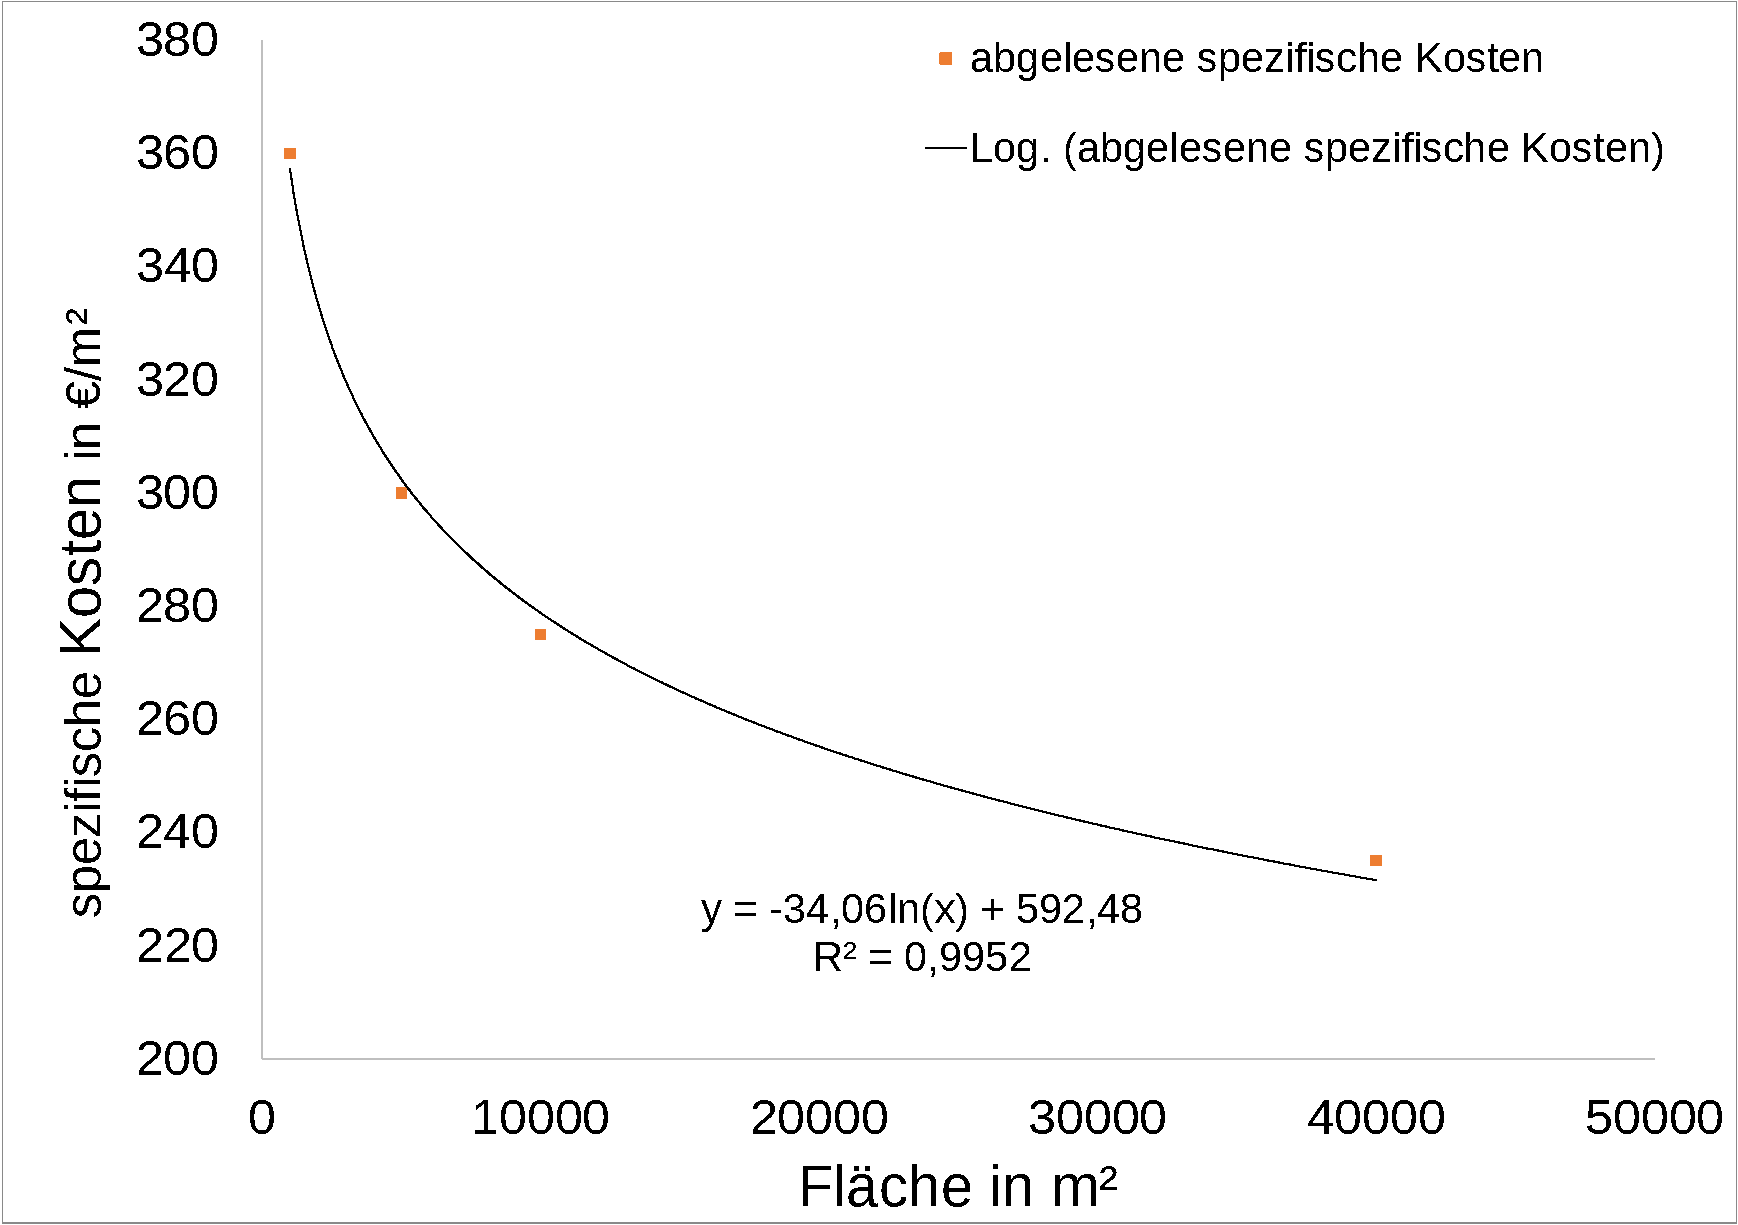
\includegraphics[width=\textwidth]{Kostendegression_Flach-cropped.pdf}
			\subcaption{Flachkollektoren}
		\end{subfigure}
		\begin{subfigure}[b]{0.49\textwidth}
			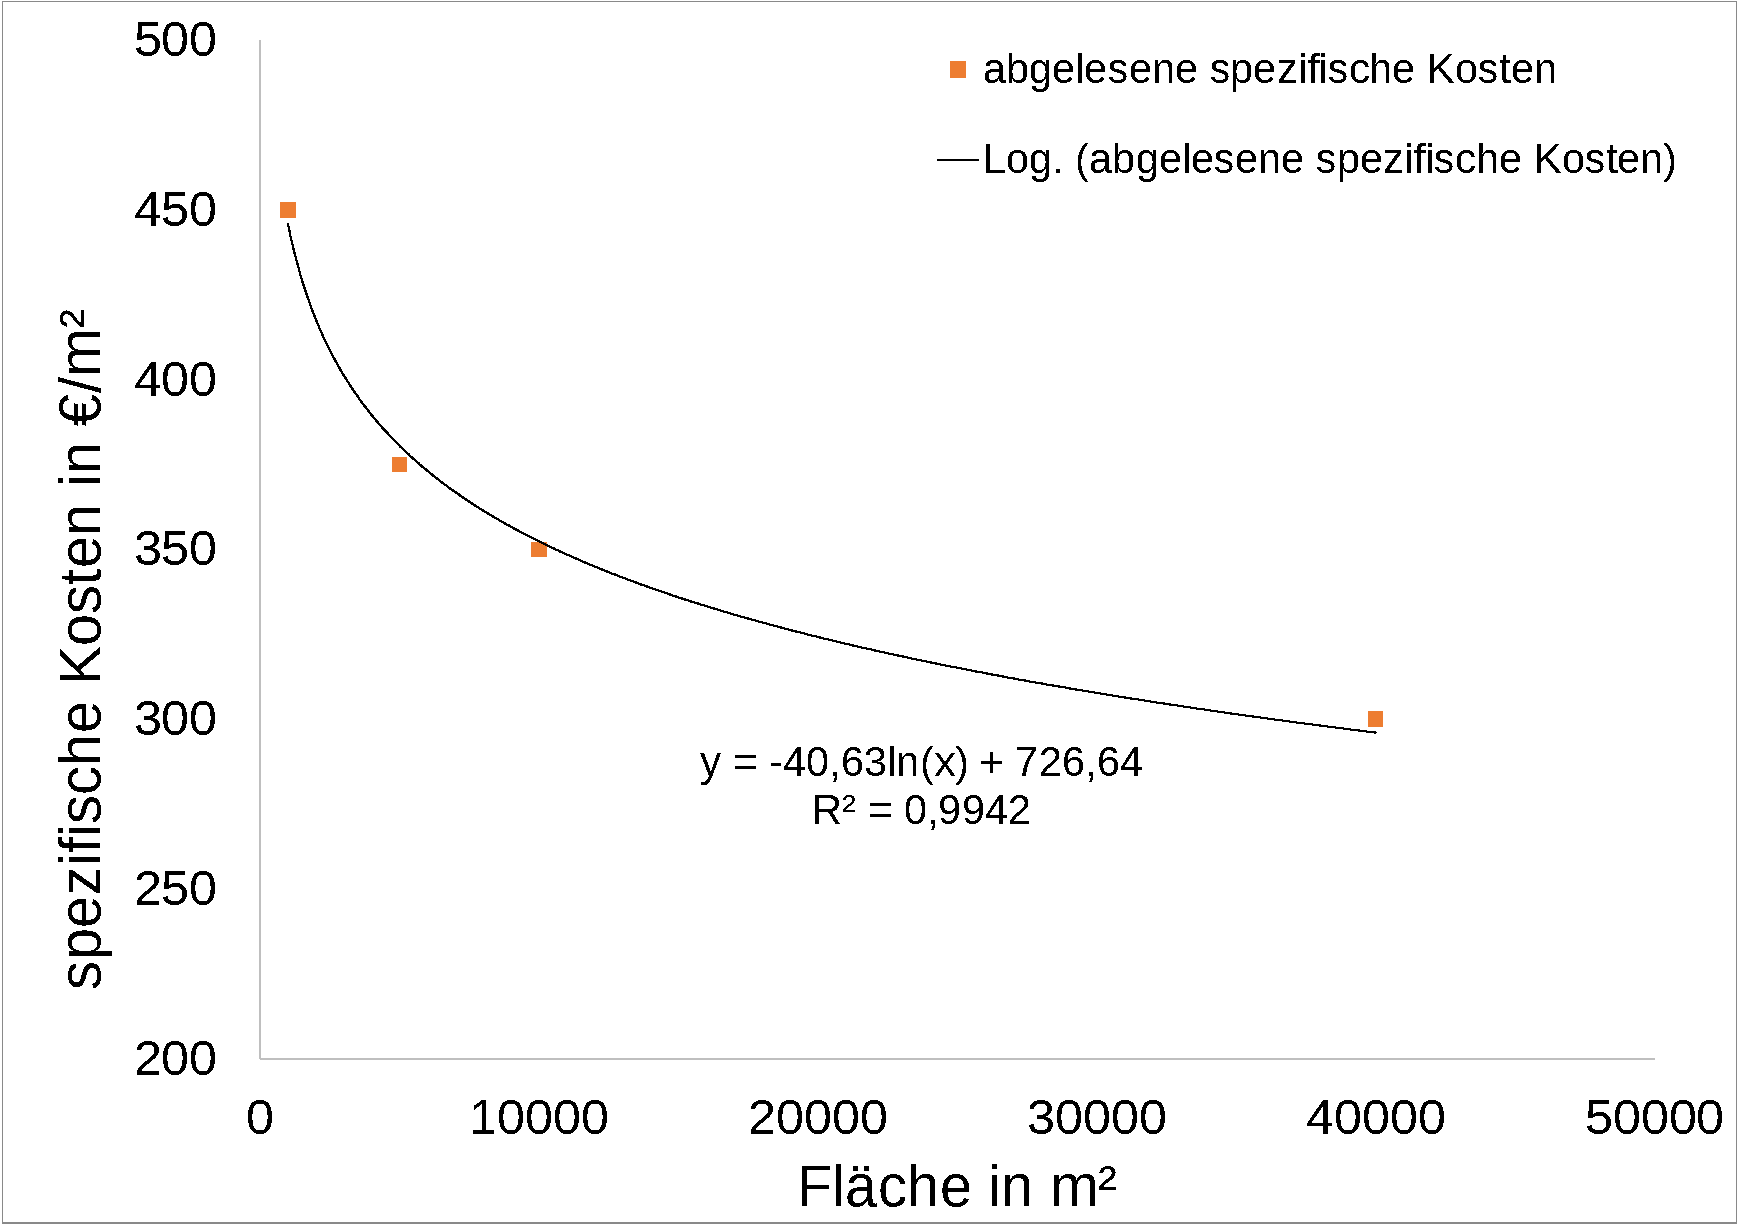
\includegraphics[width=\textwidth]{Kostendegression_Vakuum-cropped.pdf}
			\subcaption{Vakuumröhrenkollektoren}
		\end{subfigure}
		\caption[Darstellung der spezifischen Kosten für Flach- und Vakuumröhrenkollektoren]{Darstellung der spezifischen Kosten für Flach- und Vakuumröhrenkollektoren bei variierender Anlagengröße für vier ausgewählte Anlagengrößen nach \citet{Waermenetz40} sowie die Darstellung der daraus ermittelten logarithmischen Trendlinie}
		\label{fig: Kostendegression Solar}
	\end{figure}

\section{Optimierungsverfahren}\label{section: Optimierungsverfahren}
Ein stetig steigender Anteil volatiler erneuerbarer Energien an der Energieversorgung macht die Vorhersage zu erwartender Erlöse eines Energiesystems zunehmend schwierig. Betriebs- und Einsatzoptimierungen bieten eine Möglichkeit, um einen ökonomisch oder ökologisch optimalen Einsatz des Energiesystems vorherzusagen. So können Aussagen über die Wirtschaftlichkeit geplanter Anlagen getroffen und verschiedene Investitionsmöglichkeiten miteinander verglichen werden. 

In der Energietechnik haben sich lineare und gemischt-ganzzahlige Optimierungsverfahren durchgesetzt, da bei der Optimierung von Energiesystemen häufig ein ganzes Jahr als betrachteter Zeitraum verwendet wird und lange Zeitreihen zu einem überproportional steigenden Rechenaufwand führen. Lineare Probleme sind schneller zu lösen als dynamische und liefern hinreichend genaue Ergebnisse. Somit stellt die lineare Optimierung einen guten Kompromiss zwischen Rechenaufwand und Genauigkeit dar. \cite{GABRIELLI2018408}

Obwohl im Rahmen dieser Arbeit die Software \textit{Solph} genutzt worden ist (vgl. Kapitel \ref{section: Solph}), welche über die Verschaltung von vorgefertigten Komponenten automatisch die mathematische Beschreibung des Problems übernimmt, sollen die folgenden Abschnitte kurz die grundsätzliche Funktionsweise und mathematische Beschreibung der linearen und gemischt-ganzzahligen Optimierung zeigen.  

\subsection{Lineare Optimierung}
Bei der linearen Optimierung (\ac{LP}) wird das Maximum oder Minimum einer linearen Funktion, der sogenannten Zielfunktion $Z$ (objective function) gesucht. Das Überführen eines Minimierungsproblems in ein Maximierungsproblem und umgekehrt kann über die Multiplikation der Zielfunktion mit dem Faktor $(-1)$ erreicht werden. Allgemein kann die Zielfunktion wie in Gleichung \ref{equation: Zielfunktion} dargestellt werden \cite{Stoecker2008}.
	\begin{equation}\label{equation: Zielfunktion}
		\text{\textbf{min }}  Z(x_1, x_2, ..., x_n) = c_1x_1 + c_2x_2 + ... + c_nx_n = \sum_{j=1}^{n}c_jx_j
	\end{equation}
Die Zielfunktion wird aus den Strukturvariablen $x_j$ und den Strukturkonstanten $c_j$ gebildet. Die Strukturvariablen sind im Rahmen dieser Arbeit zum Beispiel die abgegebenen und aufgenommenen Wärmeströme der entsprechenden Komponenten, wohingegen die Strukturkonstanten die spezifischen Kosten der Strukturvariablen darstellen.

Die Optimierung der Zielfunktion erfolgt unter Berücksichtigung von Nebenbedingungen (Constraints). Neben den Nichtnegativitätsbedingungen, die fordern, dass die Strukturvariablen keine negativen Werte annehmen dürfen $x_j \geq 0$, werden Nebenbedingungen genutzt, um das Betriebsverhalten der Anlagen darzustellen. Allgemein werden die Nebenbedingungen als Linearkombination der Strukturvariablen dargestellt. In Gleichung \ref{equation: Nebenbedingungen} wird dies entsprechend veranschaulicht \cite{Vanderbei2014}.
	\begin{equation}\label{equation: Nebenbedingungen}
		a_1x_1 + a_2x_2 + ... +  a_nx_n \begin{Bmatrix}\geq\\=\\\leq\end{Bmatrix} b
	\end{equation} 
Ungleichungen und Gleichungen können immer ineinander überführt werden. Auf diese Weise ist das System auf eine gewünschte Form zu bringen. Können nicht alle Nebenbedingungen erfüllt werden, ist das Problem nicht lösbar (infeasible). Dementsprechend ist ein \ac{LP}-Problem lösbar (feasible), sofern alle Nebenbedingungen erfüllbar sind.

Das aufgestellte System aus Gleichungen und Ungleichungen kann unter Verwendung verschiedener Verfahren gelöst werden. Das wohl bekannteste Verfahren ist die Simplex-Methode, bei der ausgehend von einer Lösung ($x_1, x_2, ..., x_n$) iterativ nach einer anderen Lösung ($x_1^{'}, x_2^{'}, ..., x_n^{'}$) gesucht wird, die einen geringeren Wert der Zielfunktion aufweist. Dies wird so lange wiederholt, bis kein besseres Ergebnis mehr gefunden werden kann \cite{Vanderbei2014}. 

\subsection{Gemischt-ganzzahlig lineare Optimierung}
Bei der gemischt-ganzzahlig linearen Optimierung (\ac{MILP}) sind, im Gegensatz zur einfachen linearen Optimierung, alle oder wenigstens einige Variablen ganzzahlig bzw. diskret \cite{Kallrath2013}. Dies kann bei Energiesystemen zum Beispiel für Erzeugungsanlagen der Fall sein, die entweder im ein- oder ausgeschalteten Zustand sind. In diesem Fall würden die Variablen den Wert Eins oder Null annehmen. Die Verwendung des \ac{MILP}-Verfahrens erlaubt eine genauere Abbildung des Energiesystems, ist jedoch mit einem erhöhten Rechenaufwand verbunden.

Nach \citet{Kallrath2013} können aufgrund effizienterer Verfahren und besserer Solver auch komplexe und umfangreiche \ac{MILP}-Probleme in kurzer Zeit gelöst werden. Dies ist ein Grund, wieso \ac{MILP} ein Standardverfahren bei der Betriebsoptimierung in der Energietechnik ist. So wurde diese Methode unter anderem von \citet{HAIKARAINEN2014211}, \citet{GABRIELLI2018408} und \citet{MORVAJ2016619} zur Untersuchung von Solarthermie in Wärmenetzen genutzt. Im Rahmen dieser Arbeit wird ebenfalls die gemischt-ganzzahlige Optimierung verwendet.


\chapter{Grundlagen solarthermischer Wärmebereitstellung}\label{section: Solarthermische Wärmebereitstellung}
\thispagestyle{empty}

In der Literatur zu regenerativen Energiesystemen wird die Wärmegewinnung durch Solarthermie ausschließlich für die häusliche Anwendung betrachtet (\citet{Quaschning2015} und \citet{Watter2013}). Obwohl sich diese Arbeit mit dem Einsatz in Wärmenetzen  beschäftigt, bleibt die Technologie unverändert. Aus diesem Grund wird auf eine Beschreibung der Funktionsweise solarthermischer Kollektoren verzichtet. Dieser Abschnitt stellt zunächst dar, wie gemessene Daten der Sonneneinstrahlung auf eine horizontale Ebene umgerechnet werden können, um die Einstrahlung auf eine geneigte Ebene abzubilden. Anschließend wird der Ansatz zur Bewertung solarthermischen Anlagen dargestellt. Schließen wird dieser Abschnitt in einer Besprechung möglicher Konzepte zur solarthermischen Wärmebereitstellung.

\section{Funktionsweise}\label{Funktionsweise Solarthermische Wärmebereitstellung}
Bei der Solarthermie wird das Licht der Sonne in Wärme umgewandelt. Grundlage für die Berechnung solarthermischer Anlagen ist das Stefan-Boltzmann-Gesetz (Gleichung \ref{equation: Stefan-Boltzmann-Gesetz}), welches die Wärmestrahlung $\dot{Q}$ eines Körpers beschreibt \cite{stefan1879}. Die thermischen Verluste eines Kollektors, aber auch die abgegebene Strahlung der Sonne lassen sich über dieses Gesetz berechnen. 
\begin{equation}\label{equation: Stefan-Boltzmann-Gesetz}
\dot{Q} = \varepsilon \cdot \sigma_\text{s} \cdot A \cdot T^4
\end{equation}
\begin{tabbing}
	\hspace{1cm}\=\hspace{0.5cm}\=\hspace{0.5cm}\=\hspace{1cm}\=\kill
	\> $\dot{Q}$ \>: \> Wärmestrahlung eines Körpers\\
	\> $\varepsilon$ \>:  \> Emissionsgrad des Körpers\\
	\> $\sigma_\text{s}$ \>: \> Stefan-Boltzmann-Konstante\\
	\> $A$ \>: \> Oberfläche des Körpers\\
	\> $T$ \>: \> Oberflächentemperatur des Körpers\\
\end{tabbing}
Außerhalb der Erdatmosphäre beträgt die Wärmestrahlung der Sonne im Durchschnitt noch $1360,8 \pm 0,5 \frac{\text{W}}{\text{m}^2}$ \cite{Quaschning2015}. Die Strahlung, welche schließlich die Erdoberfläche erreicht, fällt aufgrund der Atmosphäre geringer aus. Gemessen wird diese Globalstrahlung $E_\text{G,hor}$ bezogen auf die horizontale Ebene \cite{DWDstrahlung}. Sie setzt sich aus einem direkten Anteil $E_\text{dir,hor}$ und einem diffusen Teil $E_\text{diff,hor}$ zusammen - dargestellt in Gleichung \ref{equation: E_hor}. Sollte bei der Messung ausschließlich die Globalstrahlung angeben sein, kann diese über statistische Verteilungen auf den direkten und diffusen Anteil umgerechnet werden \cite{Quaschning2015}.
\begin{equation}
\label{equation: E_hor}
E_\text{G,hor} = E_\text{dir,hor} + E_\text{diff,hor}
\end{equation}
Die Einstrahlung auf die horizontale Ebene ist für geneigte Kollektoren unter Berücksichtigung des Sonnenverlaufs umzurechnen, um realistische Ergebnisse für den Ertrag der Kollektoren zu erhalten. Ein möglicher Ansatz ist der in der DIN 5034-2 \cite{DIN5034} vorgeschlagenen Algorithmus zur Berechnung der Sonnenhöhe $\gamma_\text{s}$ und des Sonnenazimut $\alpha_\text{s}$. Dieser kann in Anhang \ref{Anhang: Sonnenstand} nachgeschlagen werden.

Der direkte Strahlungsanteil auf den Kollektor $E_\text{dir,gen}$ kann nach Bestimmung der entsprechenden Winkel über die in Gleichung \ref{equation: Winkelbeziehung} beschriebene Beziehung erfolgen. In Abbildung \ref{fig: Sonneneinstrahlung auf geneigter und Horizontaler Ebene} werden alle benötigten Winkel bei der Berechnung anschaulich dargestellt. Hierin stellt $\Theta_\text{gen}$ den Einfallswinkel zwischen dem Normalenvektor der Ebene und Sonne dar - $\gamma_\text{s}$ den Winkel zwischen der horizontalen und dem Sonnenstand.
\begin{equation}\label{equation: Winkelbeziehung}
E_\text{dir,gen} = E_\text{dir,hor} \cdot \dfrac{\cos \Theta_\text{gen}}{\sin \gamma_\text{s}}
\end{equation}

\begin{figure}[ht]
	\centering
	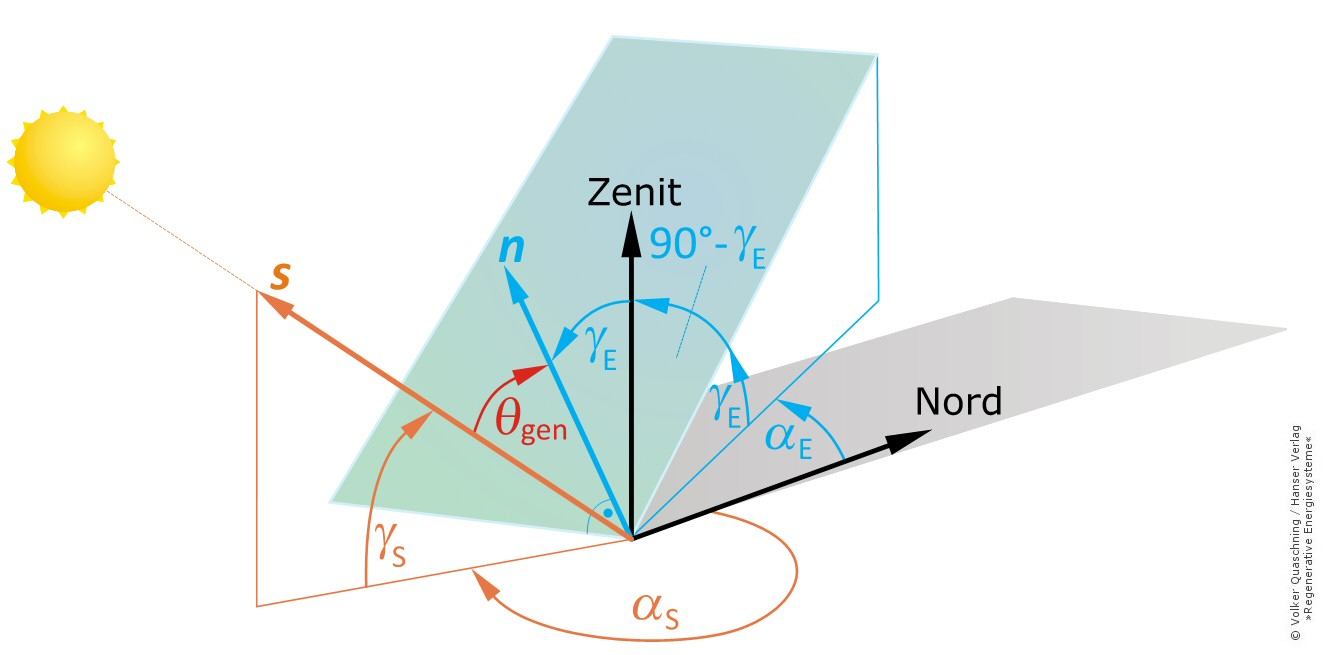
\includegraphics[width=0.8\linewidth]{Quaschning_Neigung.jpg}
	\captionof{figure}{Darstellung der Sonnenhöhe $\gamma_\text{s}$ und des Einfallswinkels $\Theta_\text{gen}$ zur Berechnung der Sonneneinstrahlung auf eine geneigte Ebene aus \citet{Quaschning2015}}
	\label{fig: Sonneneinstrahlung auf geneigter und Horizontaler Ebene}
\end{figure}
Zur Bestimmung der diffusen Einstrahlung auf die geneigte Ebene $E_\text{diff,gen}$ stehen verschiedene Ansätze zur Auswahl. In dieser Arbeit wird das Modell von \citet{KLUCHER1979} verwendet, da dieses nach \citet{Quaschning2015} eine relativ genaue Berechnung -~bei geringem Rechenaufwand~- liefert. In dem Modell von Klucher stellt der Faktor $F$ eine Hilfsgröße bei der Umrechnung dar und wird nach Gleichung \ref{equation: F} über die gemessene globale $E_\text{diff,hor}$ und diffuse Strahlung $E_\text{G,hor}$ auf die horizontale Ebene bestimmt. 
\begin{equation}
\label{equation: F}
F = 1 - \left( \dfrac{E_\text{diff,hor}}{E_\text{G,hor}} \right)^2 
\end{equation}
Dieser Faktor wird schließlich in Gleichung \ref{equation: E_diff_gen}, zusammen mit dem Aufstellwinkel der Ebene $\gamma_\text{e}$, dem Sonnenstandwinkel $\gamma_\text{s}$ und Einfallswinkel $\theta_\text{gen}$, genutzt, um die diffuse Einstrahlung auf die geneigte Ebene zu berechnen.
\begin{equation}\label{equation: E_diff_gen}
E_\text{diff,gen} = E_\text{diff,hor} \cdot \dfrac{1 + \cos \gamma_\text{s}}{2} \cdot \left( 1 + F \cdot \sin^3 \dfrac{\gamma_\text{e}}{2} \right) \cdot (1 + F \cos^2 \theta_\text{gen} \cdot \cos^3 \gamma_\text{s})
\end{equation}
Zusätzlich zur direkten und diffusen Einstrahlung auf die geneigte Ebene kommt ein kleiner Teil durch Bodenreflexion hinzu. Dieser hängt von dem Neigungswinkel $\gamma_\text{e}$ der Kollektoren und dem Albedo\footnote{Rückstrahlungsvermögen von nicht selbstleuchtenden, diffus reflektierenden Oberflächen}-Wert $A$ des Bodens ab. Die Berechnung des reflektierten Strahlungsanteils wird in Gleichung \ref{equation: E_refl_gen} dargestellt.
\begin{equation}
\label{equation: E_refl_gen}
E_\text{refl,gen} = E_\text{diff,hor} \dfrac{A (1 - \cos \gamma_\text{e})}{2}
\end{equation}
Schließlich ergibt sich die gesamte Einstrahlung  auf die geneigte Ebene nach Gleichung \ref{equation: E_G_gen} aus der Summe des direkten, diffusen und reflektierten Anteils. Abbildung \ref{fig: Vergleich horizontal vs geneigt} veranschaulicht den Gewinn, der durch die Neigung der Kollektorfläche erzielt wird.
\begin{equation}
\label{equation: E_G_gen}
E_\text{G,gen} = E_\text{dir,gen} + E_\text{diff,gen} + E_\text{refl,gen}
\end{equation}
Der gesamte DIN-Algorithmus zur Sonnenstandberechnung und Umrechnung der Einstrahlung auf die geneigte Ebene ist im Rahmen dieser Arbeit in ein Python-Skript geschrieben worden, welches dem beigefügten Datenträger entnommen werden kann.
\begin{figure}[ht]
	\centering
	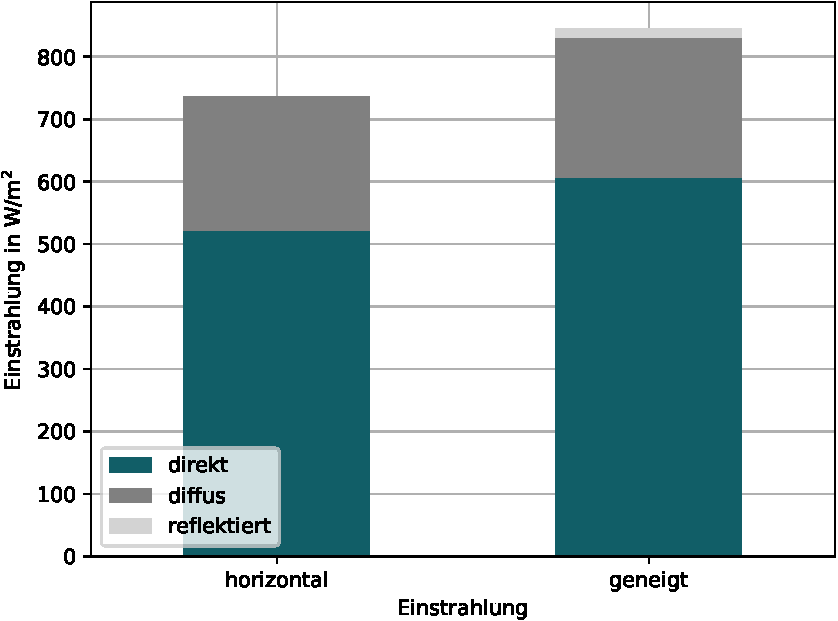
\includegraphics[width=0.8\linewidth]{radiation_on_horizontal_tilted.pdf}
	\captionof{figure}[Vergleich der Einstrahlung auf die horizontale und die geneigte Ebene]{Vergleich der Einstrahlung auf die horizontale und die geneigte Ebene. Die Rechnung ist beispielhaft für den 21.06.2016 um 14:00 Uhr, anhand der für diese Arbeit verwendeten Strahlungsdaten durchgeführt worden.}
	\label{fig: Vergleich horizontal vs geneigt}
\end{figure}

Die Effizienz $\eta_\text{K}$ der Kollektoren kann nun über den Quotienten der Nutzleistung $\dot{Q}_\text{N}$ und der  Einstrahlung auf den Kollektor mit der Fläche $A_\text{K}$ errechnet werden.
\begin{equation}\label{equation: exakter Kollektorwirkungsgrad}
\eta_\text{K} = \dfrac{\dot{Q}_\text{N}}{E_\text{G,gen} \cdot A_\text{K}}
\end{equation}	
Eine gute Annäherung für den Kollektorwirkungsgrad kann durch ein Polynom 2. Grades erreicht werden, wie es beispielsweise in DIN EN 12975 \cite{EN12975} vorgeschlagen ist. Der Wirkungsgrad wird, wie in Gleichung \ref{equation: EN12975} dargestellt, als Funktion der Temperaturdifferenz zwischen der mittleren Kollektortemperatur $T_\text{K}$ und Umgebungstemperatur $T_\text{U}$ angegeben. Dieses Verfahren wird beispielsweise von \citet{YANG2017471} zur Modellierung solarthermischer Anlagen bei einer Untersuchung zur Betriebsoptimierung in Wärmenetzen verwendet.
\begin{equation}\label{equation: EN12975}
\eta_\text{K} = \eta_\text{K,0} - \alpha_1 \cdot \dfrac{T_\text{K} - T_\text{U}}{E_\text{G,gen}} - \alpha_2 \cdot \dfrac{(T_\text{K} - T_\text{U})^2}{E_\text{G,gen}}
\end{equation}
\begin{equation}
T_\text{K} = \dfrac{T_\text{Eintritt} + T_\text{Austritt}}{2}
\end{equation}
Die Faktoren $\alpha_1$ [W/($m^2 K$)] und $\alpha_2$[W/($m^2 K^2$)] sind kollektorspezifisch und können dem Datenblatt des Herstellers entnommen werden. Der optische Wirkungsgrad $\eta_\text{K,0}$ gibt den maximal möglichen Wert an, der erreicht wird, wenn keine Temperaturdifferenz zwischen Fluid und Umgebung vorliegt. Tabelle \ref{tab: Kollektorparameter} gibt eine Übersicht über typische Werte für verschiedene Kollektorarten sowie ihre selektiven\footnote{Selektive Absorber verfügen über wellenlängenabhängige Transmissions-/Emissionskoeffizienten. Sie absorbieren Licht $< 2 \mu$m, welches den Hauptteil der Sonnenstrahlung ausmacht. Oberhalb von $2 \mu$m ist der Koeffizient möglichst gering, damit der Absorber nur wenig Wärme wieder an die Umgebung abgibt \cite{Quaschning2015}} und nicht selektiven Varianten.
\begin{center}
	\captionof{table}{Übersicht über typische Verlustkoeffizienten $\alpha_1$, $\alpha_2$ und $eta_\text{K,0}$ gängiger Kollektortypen aus \cite{Quaschning2015}}
	\begin{tabular}{llll}
		\hline 
		\rule{0pt}{12pt} Kollektortyp  & $eta_\text{K,0}$  & $\alpha_1$  & $\alpha_2$\tabularnewline
		\hline 
		
		Unverglaster Absorber  & 0,91  & 12  & 0  \tabularnewline
		Flachkollektor, Einfachverglasung, nicht selektiver Absorber & 0,86 & 6,1 & 0,025 \tabularnewline
		Flachkollektor, Einfachverglasung, selektiver Absorber  & 0,81 & 3,8 & 0,009 \tabularnewline
		Flachkollektor, Doppelverglasung, selektiver Absorber & 0,73 & 1,7 & 0,016 \tabularnewline
		Vakuumröhrenkollektor & 0,8 & 1,1 & 0,008 \tabularnewline
		\hline
		\label{tab: Kollektorparameter}  &  &  & 
	\end{tabular}
\end{center}
Das letzte Kriterium zur Bewertung solarthermischer Anlagen, welches im Rahmen dieser Arbeit Verwendung findet, ist der solare Deckungsgrad (\ac{SF}) nach Gleichung \ref{equation: SF}. Dieser gibt an, wie groß das Verhältnis aus solarthermisch gewonnener Wärme $Q_\text{ST}$ und des Wärmebedarfs $Q_\text{load}$ sowie der Wärmeverluste des Wärmenetzes $Q_\text{loss}$ ist \cite{YANG2017471}.
\begin{equation}
\label{equation: SF}
\text{\textit{SF}} = \dfrac{Q_\text{ST}}{Q_\text{load} + Q_\text{loss}}
\end{equation}

\section{Konzepte}\label{section: Konzepte}
Wie bei anderen Technologien auch, gibt es bei der Solarthermie verschiedene Möglichkeiten die Effizienz der Kollektoren oder des Gesamtsystems zu erhöhen. Die einfachste Methode stellt hier die Kombination mit anderen Wärmeversorgungstechnologien dar. \citet{ALBERGOSTERGAARD20104892} haben bereits dargelegt, dass Systeme, die einen großen Anteil regenerativer Energien aufweisen, aufgrund der volatilen Verfügbarkeit zur Versorgungssicherheit auf benachbarte Energiesysteme angewiesen sind. Entsprechend ist es bei isolierten Systemen notwendig, nicht regenerative Technologien als Back-Up zur Verfügung zu stellen. In dieser Arbeit wird ein bestehendes Versorgungssystem um drei unterschiedliche Solarthermie-Konzepte erweitert. Das bestehende System wird als Referenzsystem bezeichnet. 

Dieser Abschnitt gibt einen kurzen Überblick über verschiedene Ansätze zur Einbringung von Solarthermie in Wärmeversorgungsnetzen. Entsprechende Vor- und Nachteile der einzelnen Konzepte werden aufgeführt und eine begründete Auswahl für die drei zu untersuchenden Konzepte wird getroffen.

\subsection*{Alleinstehende Solarthermie}
Das einfachste Konzept und gleichzeitig mit den geringsten Investitionskosten ist die direkte Verwendung von solarthermischer Wärme in dem Wärmeversorgungssystem. Nachteilig bei diesem Konzept ist die Tatsache, dass Sonnenenergie zumeist dann zur Verfügung steht, wenn kein oder nur kaum Heizbedarf besteht. Eine Möglichkeit diesem Nachteil entgegen zu wirken ist die Verwendung von Wärmespeichern.

\subsection*{Solarthermie und saisonaler thermischer Energiespeicher}
	\begin{figure}[ht]
		\centering
		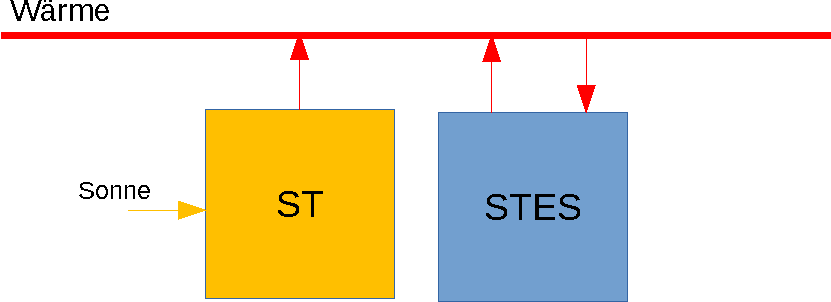
\includegraphics[width=0.8\linewidth]{ST+STES.pdf}
		\captionof{figure}[Schematische Darstellung eines Systems bestehend aus Solarthermie (ST) und einem saisonalen thermischen Energiespeichser (STES)]{Schematische Darstellung eines Systems bestehend aus einer Solarthermie-Anlage (ST), welche Sonneneinstrahlung in Wärme wandelt und an ein Wärmesystem abgibt. Ein saisonaler thermischer Energiespeicher (STES) kann zur Speicherung von Wärme genutzt werden.}
		\label{fig: ST+STES}
	\end{figure}
Dieses Konzept nutzt einen saisonalen thermischen Energiespeicher, um es zu ermöglichen, dass überschüssige solarthermische Wärme gespeichert und zu einem späteren Zeitpunkt im Wärmesystem genutzt werden kann. Abbildung \ref{fig: ST+STES} veranschaulicht dieses Konzept, welches im Folgenden auch als Basis-Solarthermie-Konzept bezeichnet wird.
Im Falle der saisonalen Speicherung entspricht dies typischerweise der Speicherung der Sonnenenergie über den Sommer und der Nutzung der gespeicherten Wärme im Winter, wenn kaum Sonnenstrahlung vorliegt und die Umgebungstemperaturen die Effizienz der Solarkollektoren soweit absenkt, dass diese nicht genutzt werden können.

\citet{CARPANETO2015714} haben bereits gezeigt, dass der Nutzen solarthermischer Anlagen durch den Einsatz von Wärmespeichern deutlich erhöht werden kann. In der Literaturrecherche zu dieser Arbeit konnte keine Quelle identifiziert werden, die Solarthermie ohne den Einsatz von Wärmespeichern untersucht. Aufgrund der Tatsache, dass es sich bei diesem Konzept um das einfachste in der Praxis verwendete Konzept handelt, ist dieses das erste, welches für eine weitere Detailuntersuchung ausgewählt wird. 

\subsection*{Solarthermie, \ac{STES} und zusätzliche Wärmequelle} 
	\begin{figure}[ht]
		\centering
		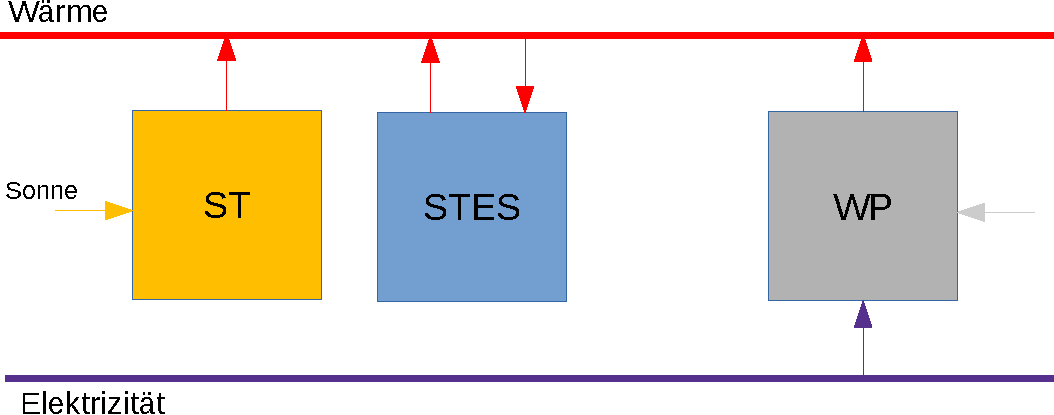
\includegraphics[width=0.8\linewidth]{ST+STES+HP1.pdf}
		\captionof{figure}[Schematische Darstellung eines um eine Kompressionswärmepumpe (WP) erweiterten Basis-Solarthermie-Konzepts]{Schematische Darstellung eines um eine Kompressionswärmepumpe (WP) erweiterten Basis-Solarthermie-Konzepts. Die Wärmepumpe nutzt Elektrizität um einen, nicht zu Heizzwecken nutzbaren Wärmestrom aufzuwerten und an das Wärmesystem abzugeben}
		\label{fig: ST+STES+HP1}
	\end{figure}
Bei diesem Konzept werden eine oder mehrere zusätzliche Wärmequellen parallel zu der Solarthermie verwendet. Diese können beispielsweise verschiedene Arten von Wärmepumpen, oder die Verbrennung von Biomasse sein. Generell lässt sich die Solarthermie mit allen möglichen Back-Up Wärmequellen kombinieren \cite{RAD20161550}. Im Rahmen dieser Arbeit wird jedoch ausschließlich die Kompressionswärmepumpe (WP) als zusätzliche Wärmequelle betrachtet, weil diese zusätzlich zur Sektorenkopplung zwischen Elektrizitäts- und Wärmeversorgung beiträgt. Außerdem weisen sie eine hohe Effizienz auf. Abbildung \ref{fig: ST+STES+HP1} zeigt das Basis-Solarthermie-Konzept, welches um eine \ac{WP} erweitert wurde, die Wärme aus der Umgebung oder Abwärme als Wärmequelle nutzt.

\subsection*{Solarthermie, \ac{STES}, \ac{WP} und \ac{STTES}}
Wärmepumpen haben den Vorteil, dass sie Phasen günstiger Strompreise nutzen können, um Wärme bereitzustellen. Diese fallen jedoch nicht unbedingt mit Bedarfsspitzen thermischer Energie zusammen. Durch die Einbringung eines Kurzzeitspeichers, der Wärme über mehrere Stunden speichern kann, ist es möglich die von der \ac{WP} bereitgestellte Wärme zeitlich von dem Bedarf zu entkoppeln. Abbildung \ref{fig: ST+STES+HP1+STTES} stellt das Konzept in einer entsprechend schematischen Darstellung vor.
	\begin{figure}[ht]
		\centering
		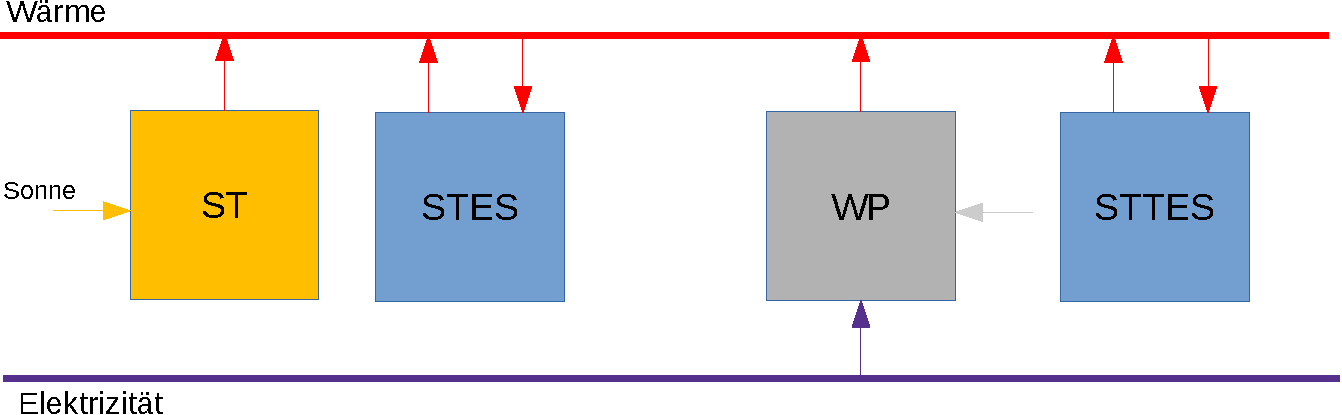
\includegraphics[width=0.8\linewidth]{ST+STES+HP1+STTES.pdf}
		\captionof{figure}[Schematische Darstellung eines Solarthermie-Konzepts mit Wärmepumpe und Kurzzeitspeicher]{Darstellung eines Basis-Solarthermie-Konzepts, welches um eine Wärmepumpe und einen Kurzzeitsspeicher erweitert worden ist. Der Kurzzeitspeicher entnimmt und beliefert das Wärmesystem mit Wärme und soll den Betrieb der Wärmepumpe optimieren}
		\label{fig: ST+STES+HP1+STTES}
	\end{figure}

Bei den zuletzt vorgestellten Konzepten sind die verwendeten Technologien ausschließlich parallel zu dem Basis-Solarthermie-Konzept geschaltet worden. Prinzipiell ein möglicher Nutzen, der durch die Verwendung einer Wärmepumpe und eines Kurzzeitspeichers erreicht wird, auch in einem Versorgungssystem ohne Solarthermie zu erwarten. 

Dieses Konzept ist für eine genauere Betrachtung im Rahmen dieser Arbeit ausgewählt worden, da durch den Einsatz einer Wärmepumpe und eines Kurzzeitspeicher das Wärmesystem einen erhöhten Anteil von \ac{P2H}-Technologien aufweist. Eine genauere Untersuchung wird zeigen, wie sich der Einsatz von Solarthermie auf ein System mit erhöhtem \ac{P2H}-Anteil auswirkt.  

\subsection*{Wärmepumpe zur Effizienzsteigerung der Solarthermiekollektoren}
Die vorangegangenen Konzepte haben ein bestehendes Solarthermie-System um weitere Technologien erweitert, die parallel zur Solaranlage geschaltet werden. Dies steigert die Effizienz des Gesamtsystems, hat jedoch keinen Einfluss auf die Effizienz der Solarthermie-Anlage. Wie aus Gleichung \ref{equation: EN12975} hervorgeht nimmt die Effizienz solarthermischer Anlagen mit abnehmender Kollektormitteltemperatur zu. Bei den bisher betrachteten Solarthermie Konzepten speist die Anlage direkt in das Wärmesystem ein. Daraus folgt, dass die Austrittstemperatur der Solaranlage mit der Vorlauftemperatur des Netzes übereinstimmt. Im Sommer liegt diese in typischen Fernwärmenetzen noch bei über 80\textdegree C \cite{stadtwerke_flensburg_gmbh_2019_2553968}. 
	\begin{figure}[ht]
		\centering
		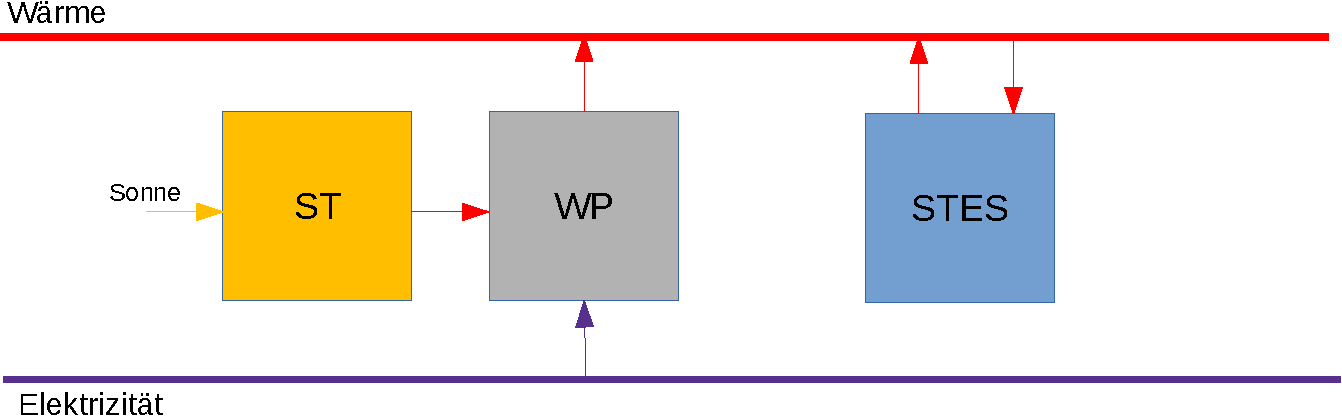
\includegraphics[width=0.8\linewidth]{ST+HP2.pdf}
		\captionof{figure}[Eine solarthermische Anlage liefert Wärme an eine Wärmepumpe zur Effizienzsteigerung]{Eine solarthermische Anlage speist in diesem Konzept nicht direkt ins Wärmesystem, sondern liefert zur Effizienzsteigerung Wärme bei einem niedrigeren Temperaturniveau an eine Wärmepumpe. Diese nutzt Elektrizität um das Temperaturniveau auf das Niveau des Wärmesystems anzuheben.}
		\label{fig: ST+HP2}
	\end{figure}

Bei diesem Konzept, welches in Abbildung \ref{fig: ST+HP2} dargestellt wird, können die Solarkollektoren auch bei geringeren Temperaturen als der Vorlauftemperatur betrieben werden, was zu einer Steigerung der Kollektoreffizienz und somit zu einem erhöhten Ertrag der Anlage führt. Außerdem kann die Wärmepumpe auch betrieben werden, wenn keine solarthermische Wärme bereitgestellt wird. Natürlich ist es ebenfalls möglich dieses Konzept  um zusätzliche Wärmequellen und Kurzzeitspeicher zu erweitern.

\subsection*{Steigerung der Speicherkapazität des \ac{STES} durch den Einsatz einer Wärmepumpe}	
Die minimale und maximale Temperatur eines Wärmespeichers ist von der Rücklauf- und maximalen Vorlauftemperatur des Wärmenetzes abhängig. Aus Gleichung \ref{equation: Speicherkapazität} geht bereits hervor, dass die Speicherkapazität direkt proportional zur Temperaturdifferenz $\Delta T$ ist. Durch den Einsatz einer Wärmepumpe kann die minimale Temperatur des Speichers unter die Rücklauftemperatur des Netzes gesenkt werden. Dieses Konzept wird in Abbildung \ref{subfigure: STES+HP3} dargestellt. 

Eine weitere Möglichkeit der Effizienzsteigerung ist die Einspeisung der solarthermischen Anlage in den Wärmespeicher anstatt direkt in das Wärmesystem einzuspeisen. Dieses Konzept, bei dem der Wärmespeicher generell bei einem geringeren Temperaturniveau betrieben wird, wurde von \citet{MARX2014} genauer betrachtet. Eine konzeptionelle Darstellung ist in Abbildung \ref{figure: ST+STES+HP3} dargestellt. Durch das reduzierte Temperaturniveau können die temperaturabhängigen Verluste verringert werden. Außerdem erhöht sich, wie im vorangegangen Konzept, die Effizienz der Solarthermie-Kollektoren. 
	\begin{figure}
		\begin{subfigure}[b]{0.48\textwidth}
			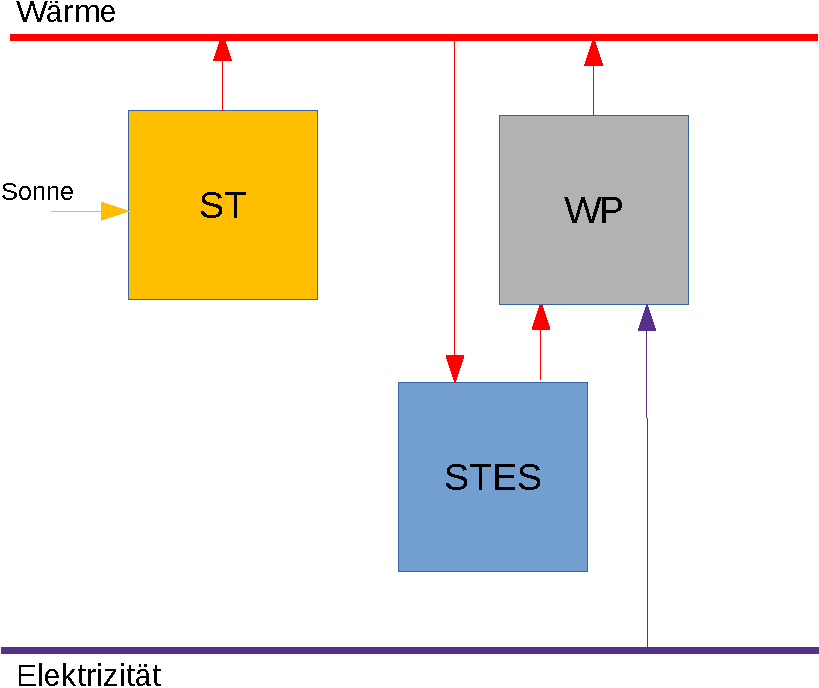
\includegraphics[width=1\textwidth]{STES+HP3.pdf}
			\subcaption{}
			\label{subfigure: STES+HP3}
		\end{subfigure}
		\hfill
		\begin{subfigure}[b]{0.48\textwidth}
			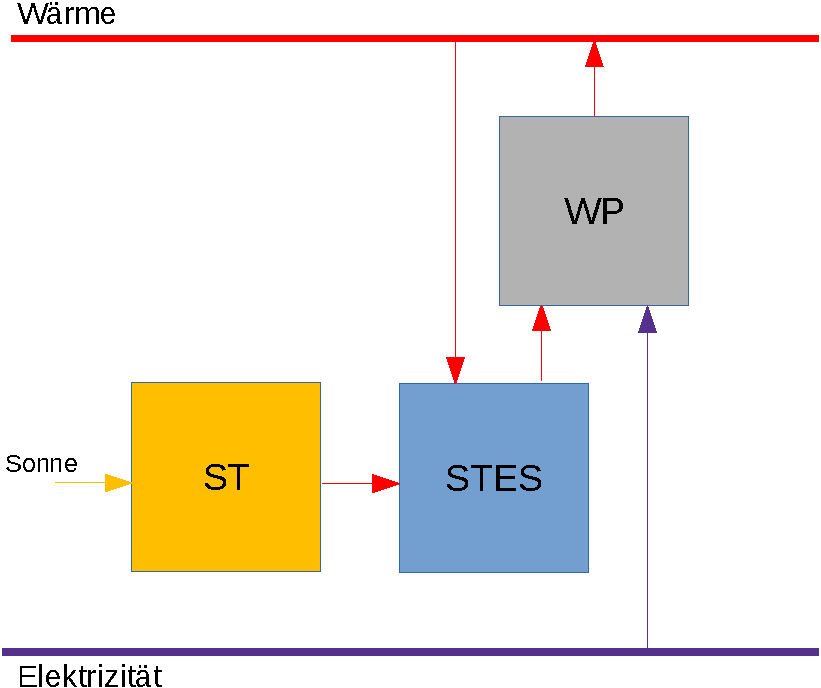
\includegraphics[width=1\textwidth]{ST+STES+HP3.pdf}
			\subcaption{}
			\label{figure: ST+STES+HP3}
		\end{subfigure}
		\caption[Konzeptionelle Darstellung zweier Ansätze zur Steigerung der Speicherkapazität durch Verwendung einer Wärmepumpe]{Konzeptionelle Darstellung zweier Ansätze zur Steigerung der Speicherkapazität durch Verwendung einer Wärmepumpe. In (a) wird eine Wärmepumpe genutzt, um einen \ac{STES} zu entladen, während eine Solarthermie-Anlage direkt ins Wärmesystem einspeist. In (b) speist die solarthermische Anlage direkt in den Speicher, der wiederum von einer Wärmepume entladen werden kann.}
		\label{fig: STES+HP}
	\end{figure}

\subsection*{Photovoltaik und Wärmepumpe}\label{subsection: Konzepte - Photovoltaik und Wärmepumpe}
	\begin{figure}[ht]
		\centering
		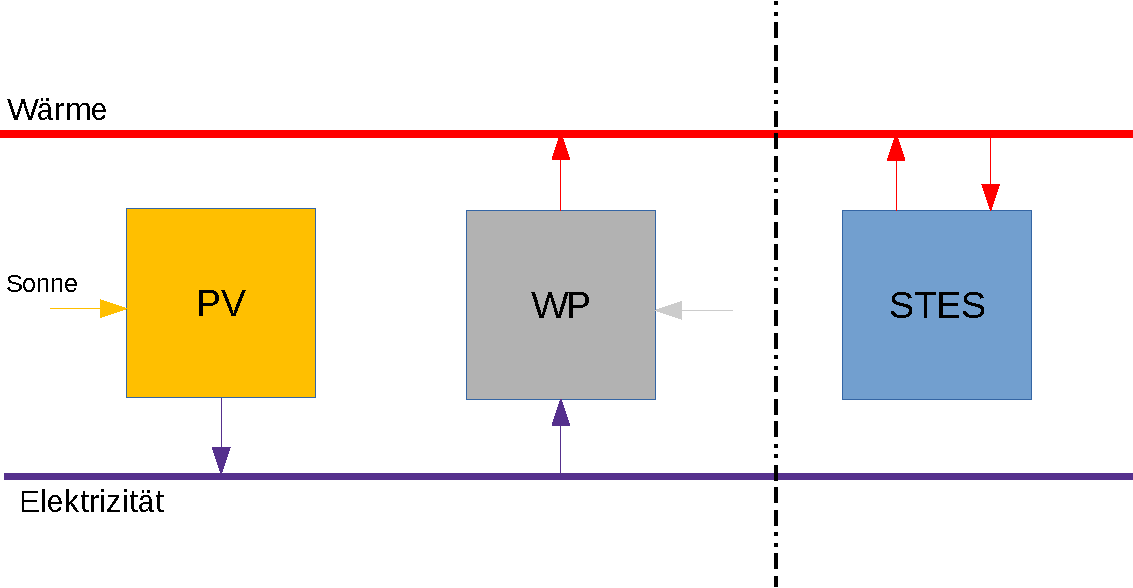
\includegraphics[width=0.8\linewidth]{Photovoltaik.pdf}
		\captionof{figure}[Schematische Darstellung eines Photovoltaik basierten Konzepts zur Wärmebereitstellung]{Schematische Darstellung eines Photovoltaik basierten Konzepts zur Wärmebereitstellung. Eine \ac{PV}-Anlage wandelt Sonneneinstrahlung in Elektrizität um, die wiederum von der Wärmepumpe genutzt werden kann, um Wärme bereitzustellen.}
		\label{Abbildung: PV-Konzept}
	\end{figure}
\citet{GRAVELSINS2019} haben ein Konzept vorgestellt, welches eine Alternative zur klassischen Solarthermie darstellt, in dem die Sonnenstrahlung indirekt genutzt wird, um Wärme bereitzustellen. Der durch die \ac{PV}-Anlage gewonnene Strom wird genutzt, um eine Wärmepumpe zu betreiben, die wiederum dem Wärmenetz Wärme bereitstellt. Dieses Konzept der \textit{indirekten} Solarthermie, welches in Abbildung \ref{Abbildung: PV-Konzept} dargestellt wird, bietet einige Vorteile gegenüber der klassischen Solarthermie. Zunächst haben \ac{PV}-Module den Vorteil, dass sie schwankenden Umgebungsbedingungen gegenüber unempfindlicher sind als Solarthermieanlagen. Eine sinkende Umgebungstemperatur hat beispielsweise, im Gegensatz zur Solarthermie, einen positiven Einfluss auf den Modul-Wirkungsgrad \cite{Quaschning2015}. Ein weiterer Vorteil ist, dass  die erforderliche Wärmepumpe einerseits unabhängig von der dargebotenen Strahlung eingesetzt und andererseits der \ac{PV}-Strom - je nach Preislage und Wärmenachfrage - direkt vermarktet werden kann.  

Ein weiterer Vorteil des \ac{PV}-Konzepts ist, dass die Investitionskosten von \ac{PV}-Modulen pro m² derzeit deutlich geringer ausfallen als bei Flach- oder Vakuumröhrenkollektoren. Darüber hinaus haben \citet{Vartiainen2019} dargelegt, dass in den nächsten Jahren weiter mit stark fallenden Preisen für die Photovoltaik zu rechnen ist. Tabelle \ref{tab: Preisvergleich PV/Solar} stellt die aktuellen Investitionskosten der verschiedenen Technologien von Anlagen jenseits der 100.000m² - die in Dänemark bereits eingesetzt werden - vergleichend gegenüber. Die Kosten für \ac{PV} sind \textit{Aktuelle Fakten zur Photovoltaik} \cite{ISE} entnommen worden, die Kosten der Solarthermie sind nach Gleichung \ref{equation: Kosten-Flachkollektor} und \ref{equation: Kosten-Vakuumkollektor} bestimmt worden. Aufgrund der zu erwartenden, anhaltenden Kostenreduktion von \ac{PV}-Modulen und der vielfältigen Möglichkeiten die Sonnenstrahlung zu nutzen ist dieses Konzept als drittes für eine weitere Detailanalyse ausgewählt worden.
\newpage
	\begin{center}
		\captionof{table}{Gegenüberstellung der spezifischen Investitionskosten zwischen Photovoltaik und Solarthermie für Anlagen > 100.000m²}
		\begin{threeparttable}
		\begin{tabular}{lcccl}
			\hline 
			\rule{0pt}{12pt} Technologie  & Einheit & Preis & Quelle & rel. Preis\tabularnewline
			\hline
			Photovoltaik (monokristallin)  &  \euro / kW$_\text{p}$ &  600 - 800 & \cite{ISE} & 1  \tabularnewline
			 & \euro/m² & $\approx$ 120 & & 1 \tabularnewline
			Flachkollektor & \euro/m²  & 190 & \cite{Waermenetz40}\tnote{1} & 1,6\tabularnewline
			Vakuumröhrenkollektor & \euro/m² & 245 & \cite{Waermenetz40} & 2,1\tabularnewline
			\hline
		\end{tabular}
		\begin{tablenotes}\footnotesize 
			\item[1] Grundlage für die Preisberechnung bildet \citet{Waermenetz40} (vgl. Gleichung \ref{equation: Kosten-Flachkollektor} und \ref{equation: Kosten-Vakuumkollektor}).
		\end{tablenotes}
	\end{threeparttable}
		\label{tab: Preisvergleich PV/Solar}
	\end{center} 
Folgende drei Konzepte werden im Rahmen dieser Arbeit weiter untersucht:
	\begin{description}
		\item[Solarthermie 1] Solarthermie und ein saisonaler thermischer Energiespeicher ergänzen das bestehende Referenzsystem. Diese Variante stellt das einfachste, aber zugleich das grundlegende solarthermische Konzept dar und ist aus diesem Grund als erstes Konzept für eine Detailuntersuchung ausgewählt worden.

		\item[Solarthermie 2] Hier wird das Solarthermie 1 Konzept zusätzlich um eine Wärmepumpe und einen Kurzzeitspeicher erweitert. Es ist ausgewählt worden, um den Einfluss der Solarthermie auf ein Wärmesystem mit erhöhtem \ac{P2H}-Anteil zu untersuchen.
		
		\item[Photovoltaik] Dieses Konzept stellt eine alternative Möglichkeit der solarthermischen Wärmebereitstellung dar. Die Solarthermie-Kollektoren sind durch eine Kombination aus \ac{PV}-Modulen und Wärmepumpen ersetzt worden. Dieses Konzept wurde ausgewählt, um zwei grundlegend verschiedene Konzepte zur Wärmebereitstellung aus Sonnenenergie miteinander zu vergleichen.		
	\end{description}
\chapter{Modellbildung}\label{chapter: Modellbildung}
\thispagestyle{empty}
Dieses Kapitel stellt dar, wie die verwendeten technischen Anlagen zur Gewinnung von Betriebskennlinien modelliert worden sind. Im ersten Abschnitt wird die verwendete Simulationssoftware \acf{TESPy} vorgestellt. Daran anschließend wird für jede Technologie gezeigt, wie diese in \ac{TESPy} modelliert wurde und welche Daten bzw. Kennlinien konkret aus der Simulation gewonnen werden konnten - alle Modelle können dem beigefügten Datenträger entnommen werden. Außerdem wird gezeigt wie gewonnene Kennlinien für die spätere Optimierung linearisiert worden sind. 

\section{Simulationssoftware - TESPy}\label{section: TESPy}
\ac{TESPy} ist ein Python-Paket, welches zur Simulation thermodynamischer Kreisprozesse genutzt werden kann. Im Rahmen dieser Arbeit ist \ac{TESPy} verwendet worden, um die Erzeugungsanlagen der untersuchten Energiesysteme abzubilden und Wirkungsgrad-Kennlinien für die \ac{MILP}-Optimierung zu gewinnen. 

Bei \ac{TESPy} handelt es sich um ein komponentenbasiertes Simulationsprogramm in dem vordefinierte Komponenten, wie beispielsweise Turbinen, Pumpen oder Wärmeübertrager miteinander verbunden werden können, um komplexere technische Anlage (zum Beispiel ein Kraftwerk) abzubilden. Es ist möglich diese Anlagen für einen bestimmten, vordefinierten Betriebspunkt auszulegen. Ausgehend von diesem Punkt ist es über hinterlegte Betriebscharakteristiken ebenfalls möglich das Teillastverhalten dieser Anlage zu simulieren. 

Das durch verbinden einzelner Komponenten erstellte Netzwerk wird in \ac{TESPy} als Gleichungssystem nicht linearer Gleichungen dargestellt, welches über das mehrdimensionale Newton-Raphson-Verfahren gelöst wird. Bei diesem Verfahren handelt es sich um ein numerisches Lösungsverfahren, welches iterativ eine mögliche Nullstelle annähert. Die Anzahl der für das Newton-Raphson-Verfahren benötigten Variablen kann Gleichung \ref{equation: nvariables} entnommen werden \cite{TESPy2019}.
	\begin{equation}\label{equation: nvariables}
		n = \text{\textit{num}}_\text{conn} \cdot (3 + \text{\textit{num}}_\text{fluids})
	\end{equation}
Im Folgenden wird anhand eines einzelnen Solarkollektors, welcher Wasser mit einer Temperatur von 20\textdegree C und einem Druck von 5 bar auf eine Temperatur von 50\textdegree C erwärmt, die Anwendung von TESPy veranschaulicht. Zunächst muss ein Netzwerk erstellt werden, dem die Komponenten und Verbindungen im späteren Verlauf hinzugefügt werden:

\begin{lstlisting}[language=python,numbers=none]
from tespy import con, nwk, cmp	
nw = nwk.network(fluids=['water'])
nw.set_attr(p_unit='bar', T_unit='C', h_unit='kJ / kg')
\end{lstlisting}
Anschließend werden die verwendeten Komponenten definiert - in diesem Fall der Kollektor, sowie eine Quelle und Senke:
\begin{lstlisting}[language=python,numbers=none]
source = cmp.source('Wasser-Quelle')
collector = cmp.solar_collector('Solarkollektor')
sink = cmp.sink('Wasser-Senke')
\end{lstlisting}
Nun können die Komponenten miteinander verbunden und dem Netzwerk hinzugefügt werden:
\begin{lstlisting}[language=python,numbers=none]
source.collector = con.connection(source, 'out1', collector, 'in1')
collector.sink = con.connection(collector, 'out1', sink, 'in1')
nw.add_conns(source.collector, collector.sink)
\end{lstlisting} 
Bevor das Netzwerk simuliert werden kann sind die Komponenten und Verbindungen zu parametrisieren. Hier stehen eine Vielzahl von Parametern zur Verfügung, die in der Dokumentation \cite{TESPy2019} nachgeschlagen werden können. In diesem Beispiel wird ein Kollektor mit einer Fläche von 2,5 $\text{m}^2$ bei einer Außentemperatur von 20\textdegree C und einer Sonneneinstrahlung von 600 W/m$^2$ simuliert. Darüber hinaus ist der Kollektor mit einem linearen $lkf_{lin}$ und quadratischen Wärmeverlustkoeffizienten $lkf_{quad}$ versehen.
\begin{lstlisting}[language=python,numbers=none]
collector.set_attr(Tamb=20, A=2.5, lkf_lin=1.1, lkf_quad=0.008, E=600)
	
source.collector.set_attr(T=20, p=5, fluid={'water': 1})
collector.sink.set_attr(T=50, p=5)
\end{lstlisting}
Abschließend wird die Simulation gestartet und die abgegebene Heizleistung des Kollektors bestimmt. Die Ergebnisse der Simulation können über den Befehl nw.save gespeichert werden:
\begin{lstlisting}[language=python,numbers=none]
nw.solve(mode='design')
nw.save('Solarkollektor')
		
Heizleistung: 1447.5 W
\end{lstlisting}
Um die Anlage in Teillast zu simulieren muss der Modus von \textit{Design} auf \textit{Offdesign} geändert werden. Außerdem muss die gespeicherte Datei \textit{Solarkollektor} als Design-Datei angegeben werden. Zusätzlich ist zu definieren wie sich die Komponenten im Teillastbetrieb verhalten sollen. Zum grundsätzlichen Verständnis wie \ac{TESPy} funktioniert soll jedoch die Beschreibung des Auslegungsfalls ausreichen.
 

\section{Solarthermie}\label{section: Modellbildung - Solarthermie}
Die Fläche, die benötigt wird, um Wärmeversorgungsnetze nennenswert unterstützen zu können ist erheblich und mit häuslichen Anwendungen nicht zu vergleichen. Dänemark - Vorreiter bei der solarthermischen Wärmeversorgung - verfügt über 50 Anlagen, die eine Kollektorfläche von 10.000 m$^2$ übersteigen \cite{SDH2019}. Anlagen solcher Größe werden über die Verschaltung herkömmlicher Solarkollektoren, welche auch im privaten Sektor zum Einsatz kommen, realisiert. In Kapitel \ref{section: Solarthermische Wärmebereitstellung} ist zur Beschreibung eines Kollektors bereits auf die DIN EN 12975 \cite{EN12975} (wird ebenfalls von \ac{TESPy} zur Berechnung des Solarkollektors genutzt) hingewiesen worden. Diese ist zunächst jedoch nur für einen einzelnen Kollektor geeignet. Es stellt sich also die Frage, welchen Einfluss die Verschaltung mehrerer Kollektoren auf das Verhalten der Gesamtanlage hat. Grundsätzlich können Kollektoren auf zwei Arten verschaltet werden - Parallel und in Reihe.
	\begin{center}
		\captionof{table}{Parameter der verwendeten Vakuumröhren- und Flachkollektoren}
		\begin{threeparttable}
			\begin{tabular}{llcll}
				\hline 
				\rule{0pt}{12pt} Parameter  & Symbol  & Einheit  & \multicolumn{2}{c}{Kollektortyp}\tabularnewline
				& & & Vakuum & Flach \tabularnewline
				\hline 
				\textbf{Kollektor}  &  &  &  &\tabularnewline
				optischer Wirkungsgrad  & $\eta_\text{K,0}$ & - & 0,8 & 0,73 \tabularnewline
				linearer Verlustkoeffizient & $\alpha_1$  & W/(m$^2$K) & 1,1 & 1,7 \tabularnewline
				quadratischer Verlustkoeffizient & $\alpha_2$ & W/(m$^2$K$^2$) & 0,008 & 0,016 \tabularnewline
				Fläche & A & m$^2$ & \multicolumn{2}{c}{2,5}\tabularnewline
				Aufstellwinkel  & $\gamma_\text{e}$ & \textdegree & \multicolumn{2}{c}{37\tnote{1}}\tabularnewline
				Ausrichtung des Moduls  & - & - & \multicolumn{2}{c}{Süden} \tabularnewline
				\textbf{Fernwärmenetz und Umgebung}  &  &  &  &\tabularnewline
				Rücklauftemperatur  & $\vartheta_\text{RL} = T_\text{Eintritt}$  & \textdegree C  & \multicolumn{2}{c}{50} \tabularnewline
				Vorlauftemperatur & $\vartheta_\text{VL} = T_\text{Austritt}$ & \textdegree C & \multicolumn{2}{c}{81} \tabularnewline
				Umgebungstemperatur  & $T_\text{U}$ & \textdegree C & \multicolumn{2}{c}{16} \tabularnewline
				\hline
				
			\end{tabular}
			\begin{tablenotes}\footnotesize 
				\item[1] Bei diesem Winkel wird der Ertragsgewinn durch die Neigung der Kollektoren maximal - bezogen auf die vorliegenden Wetterdaten.
			\end{tablenotes}
		\end{threeparttable}
		\label{tab: verwendete Kollektordaten}
	\end{center} 

Die Parallelschaltung hat offensichtlich kaum einen Einfluss auf das Betriebsverhalten - es könnten ebenso mehrere separate Anlagen betrieben werden. Interessant ist jedoch das Verhalten der Kollektoren in Reihenschaltung, durch die - bei gleichem Massenstrom - deutlich höhere Austrittstemperaturen als bei der Parallelschaltung erreicht werden können \cite{Watter2013}. In der Praxis ist eine Kombination aus beiden Varianten gängig.  
Aus Gleichung \ref{equation: EN12975} geht hervor, dass bei steigender Kollektortemperatur der Wirkungsgrad abnimmt. Somit sinkt mit jedem zusätzlichen Kollektor dessen Wirkungsgrad.
	\begin{figure}
		\centering
		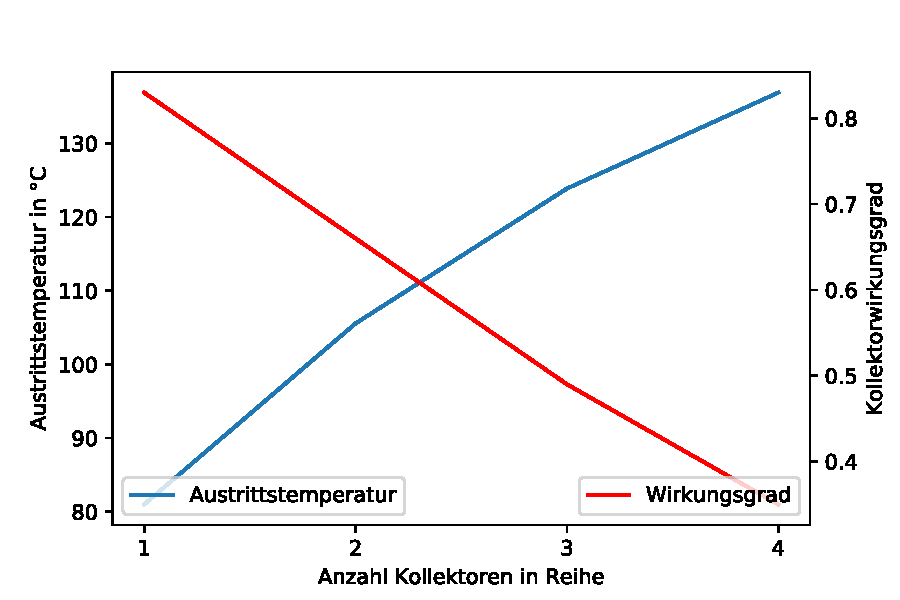
\includegraphics[width=0.8\linewidth]{Kollektortemperaturen.pdf}
		\captionof{figure}[Darstellung der Temperatur und des Wirkungsgrads einzelner Vakuumröhrenkollektoren mit zunehmender Kollektoranzahl]{Darstellung der Temperatur und des Wirkungsgrads einzelner Vakuumröhrenkollektoren mit zunehmender Kollektoranzahl bei gleichbleibendem Massenstrom. Während die Austrittstemperatur mit jedem zusätzlichen Kollektor zunimmt, sinkt der Wirkungsgrad des letzten Kollektors in Reihe.}
		\label{fig: Kollektortemperatur und Wirkungsgrad über Kollektoranzahl}
	\end{figure}
Abbildung \ref{fig: Kollektortemperatur und Wirkungsgrad über Kollektoranzahl} zeigt die entsprechende Abhängigkeit von der Austrittstemperatur. Der Verlauf des Wirkungsgrads impliziert, dass bei einer bestimmten Kollektoranzahl in Reihe der letzte Kollektor irgendwann - je nach Randbedingungen - einen negativen Wirkungsgrad aufweisen wird. Die Simulation in TESPy hat gezeigt, dass mehr Vakuumröhrenkollektoren als Flachkollektoren in Reihe geschaltet werden können, bevor der Wirkungsgrad negative Werte annimmt. Demgegenüber steht, dass Flachkollektoren derzeit die geringeren Investitionskosten aufweisen. Tabelle \ref{tab: verwendete Kollektordaten} gibt eine Übersicht über die wichtigsten Parameter bei der Simulation der Kollektoren. Das komplette \ac{TESPy}-Skript ist dem beigefügten Datenträger zu entnehmen.

Für die Optimierung eines solarthermisch gestützten Wärmesystems gilt es nun herauszufinden, welchen Einfluss eine Reihenschaltung auf den Wirkungsgrad des Gesamtsystems hat. Zu diesem Zweck sind für bis zu vier Kollektoren in Reihe die Systemwirkungsgrade über der Sonneneinstrahlung untersucht worden. Es zeigt sich, dass bei festgehaltener Austrittstemperatur eine Zunahme der Kollektoranzahl auf zwei, drei oder vier Kollektoren der Wirkungsgrad insgesamt relativ konstant bleibt. Bei geringer Einstrahlung ist eine leichte Abnahme des Wirkungsgrad mit zunehmender Kollektoranzahl zu beobachten. Bei einer höheren Einstrahlung von 600~W/m² bis 1000~W/m² ist praktisch kein Unterschied zu erkennen. Dieser Sachverhalt wird in Abbildung \ref{fig: TESPy Vergleich mehrerer Kollektoren in Reihe} dargestellt. Dieses Verhalten ist damit zu erklären, dass bei festgehaltener Reihen-Austrittstemperatur der Wirkungsgrad der hinteren Kollektoren sinkt, dem gegenüber jedoch eine Wirkungsgrad-Zunahme der vorderen Kollektoren, aufgrund der jeweils abnehmenden Kollektor-Austrittstemperatur, steht. 
	\begin{figure}[ht]
		\centering
		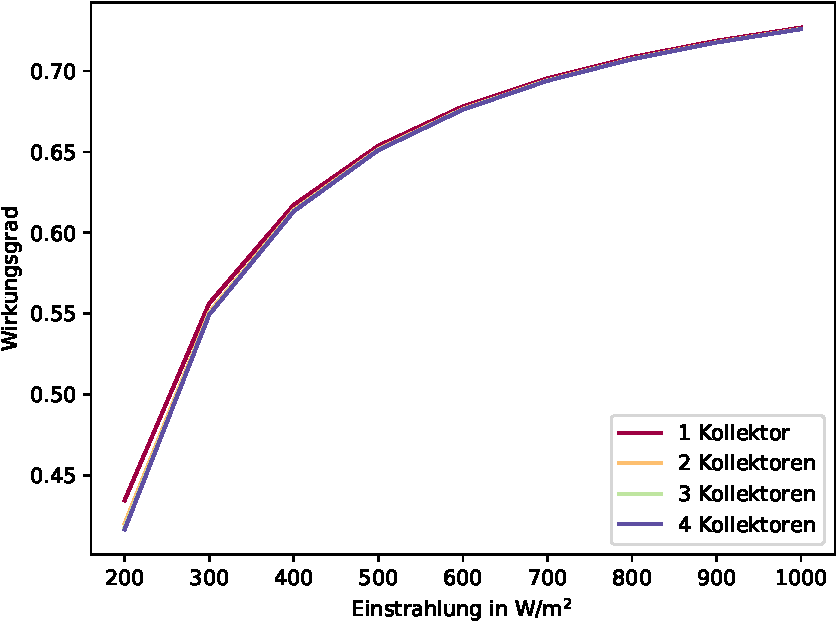
\includegraphics[width=0.8\linewidth]{Kollektor_eta_Reihe-cropped.pdf}
		\captionof{figure}[Vergleich des Gesamt-Wirkungsgrads mit zunehmender Kollektoranzahl in Reihe]{Darstellung des Gesamt-Wirkungsgrads mit zunehmender Kollektoranzahl in Reihe über einer variierenden Einstrahlung bei festgehaltener Austrittstemperatur anhand einer eigenen \ac{TESPy}-Simulation. Die Steigerung der Kollektoranzahl führt bei geringer Einstrahlung zu einer leichten Verringerung des Wirkungsgrads. Bei höherer Einstrahlung ist dieser Effekt nicht zu beobachten.}
		\label{fig: TESPy Vergleich mehrerer Kollektoren in Reihe}
	\end{figure}

Auf Grundlage der \ac{TESPy}-Simulation ist entschieden worden, die gewonnene Wärme des Kollektorfeldes über die DIN EN 12975 \cite{EN12975} für jeden Zeitschritt im Preprocessing zu berechnen und als Wert an Solph zu übergeben. Da der Unterschied zu einem einzelnen Kollektor quasi unerheblich ist, kann die DIN-Vorschrift bedenkenlos eingesetzt werden. Der Ertrag wurde folgendermaßen bestimmt:
	\begin{enumerate}
		\item Umrechnung der vorhandenen Einstrahlungsdaten auf die geneigte Ebene
		\item Nutzen der Vorlauf-, Umgebungstemperatur und Einstrahlungsdaten (vgl. Kapitel~\ref{section: Eingangsparameter der Optimierung}) zur Bestimmung des Kollektorwirkungsgrads nach DIN~EN~12975
		\item Berechnung des flächenspezifischen Ertrags der Solarthermie
	\end{enumerate} 

Auf Grund der Tatsache, dass der Wirkungsgrad eines Vakuumröhrenkollektors tendenziell höher ist, als der von Flachkollektoren ist entscheiden worden im weiteren Verlauf dieser Arbeit auf die Betrachtung von Flachkollektoren zu verzichten.

\section{Gas- und Dampfkraftwerk}\label{section: Gas- und Dampfkraftwerk}
Unter den verschiedenen Technologien der Kraft-Wärme-Kopplung ist das \acl{GuD} eine der bewährtesten Varianten. Die Abwärme der Gasturbine wird genutzt, um einen Dampfkreislauf zu betreiben und so die Brennstoffausnutzung weiter zu erhöhen. Im Vergleich zu Braun- oder Steinkohle gefeuerten Kraftwerken ist die CO$_2$-Emission von Gas gefeuerten Kraftwerken bezogen auf die Kilowattstunde Strom um mehr als die Hälfte geringer \cite{statista2019}. Der geplante Kohleausstieg der Bundesregierung für das Jahr 2038 erhöht die Bedeutung der \ac{GuD} weiter \cite{bmwi2019}. Aus diesem Grund wird in dieser Arbeit die \ac{GuD}-Technologie im Referenzsystem zur primären Wärmeversorgung verwendet.
	\begin{figure}[h]
		\centering
		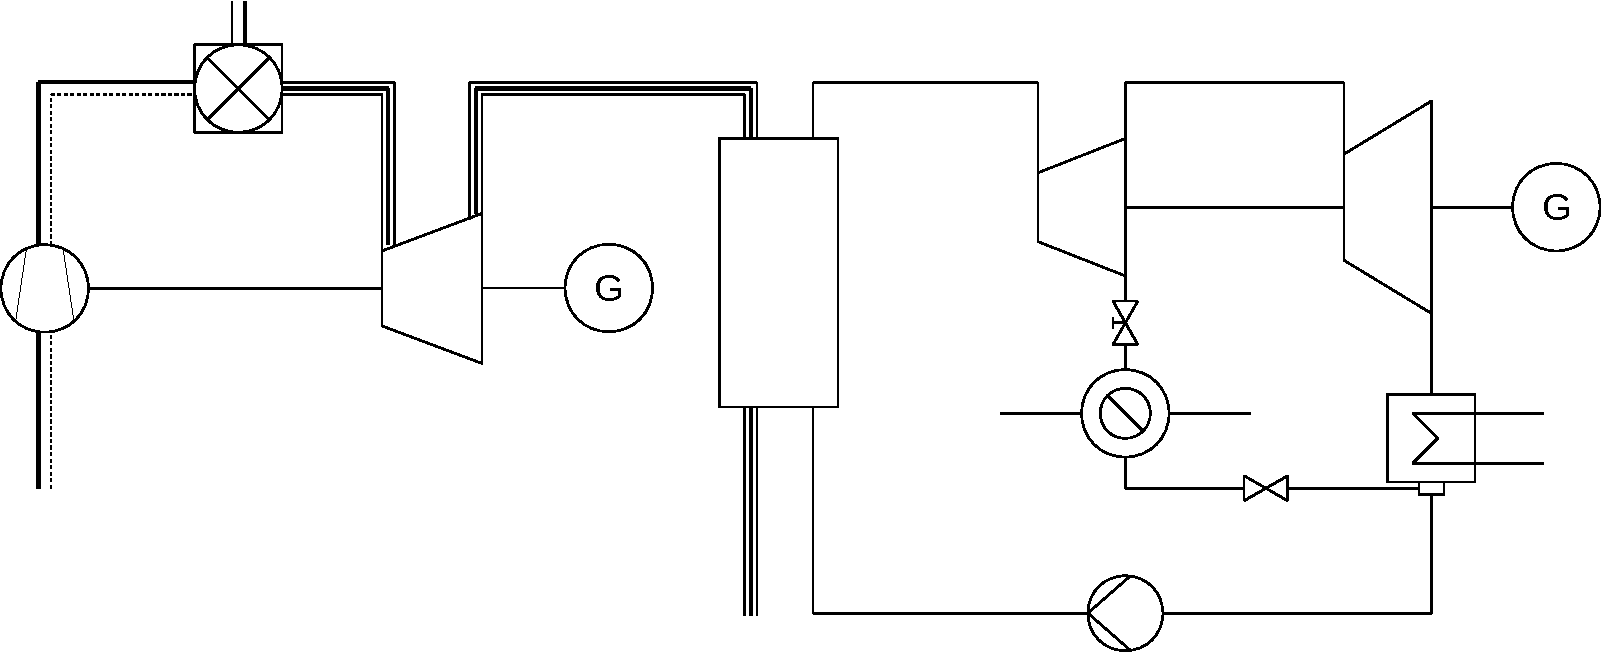
\includegraphics[width=0.8\linewidth]{SchaltplanGuD.pdf}
		\captionof{figure}{Wärmeschaltbild des in \ac{TESPy} modellierten \acl{GuD}s mit einer einfachen Entnahmeschaltung}
		\label{fig: Schaltplan GuD-Anlage}
	\end{figure}

Das verwendete Simulationsprogramm zur Optimierung des Energiesystems (Solph), auf das in Kapitel \ref{section: Solph} weiter eingegangen wird, verfügt bereits über eine \ac{GuD}-Komponente, die \textit{GenericCHP}, welche das Verhalten dieses Anlagentyps sehr genau beschreibt. Für eine detailliertere Beschreibung dieser Komponente wird entsprechend auf die \ac{oemof}-Dokumentation \cite{oemof2019} oder die Veröffentlichung von \citet{Mollenhauer2016} verwiesen, auf deren Grundlage die GenericCHP modelliert wurde. Um die GenericCHP-Komponente verwenden zu können sind nur einige Eckdaten nötig, die entsprechend über eine \ac{TESPy}-Simulation ermittelt worden sind. Die gewonnenen Eckdaten können in Tabelle \ref{tab: Notwendige Eckdaten zur Verwendung der GenericCHP-Komponente} nachgelesen werden.

Abbildung \ref{fig: Schaltplan GuD-Anlage} zeigt eine schematische Darstellung des modellierten Kraftwerks. Das nach der Expansion in der Gasturbine immer noch heiße Gas wird in einem Abhitzekessel genutzt, um Wärme für einen Dampfkraftprozess bereitzustellen. Der Dampfkreislauf ist als Entnahme-Kondensation ausgeführt, was bedeutet, dass Dampf der Turbine auf einem erhöhten Druckniveau zu Heizzwecken entnommen wird. Der Dampf wird in einem Heizkondensator kondensiert und gibt dabei Wärme an das Wärmenetz ab. Der in der Turbine verbleibende Dampf wird weiter auf einen niedrigeren Druck expandiert. Tabelle \ref{tab: Nennparameter GuD} fasst die wichtigsten Parameter zur Simulation des Kraftwerks zusammen.
	\begin{center}
		\captionof{table}{Notwendige Eckdaten zur Verwendung der GenericCHP-Komponente}
		\begin{tabular}{llll}
			\hline 
			\rule{0pt}{12pt} Parameter  & Symbol  & Einheit  & Wert \tabularnewline
			\hline 
			maximale elektrische Leistung ohne Wärmeauskopplung  & $P_\text{max,woDH}$ & MW & 406  \tabularnewline
			minimale elektrische Leistung ohne Wärmeauskopplung & $P_\text{min,woDH}$ & MW & 139 \tabularnewline
			maximale Stromausbeute ohne Wärmeauskopplung &  $\beta_\text{max,woDH}$  & - & 0,5851 \tabularnewline
			minimale Stromausbeute ohne Wärmeauskopplung &  $\beta_\text{min,woDH}$  & - & 0,4798 \tabularnewline
			Leistungs-Verlust-Index &  $beta$  & - & 0,2447 \tabularnewline
			\hline
			\label{tab: Notwendige Eckdaten zur Verwendung der GenericCHP-Komponente}  &  &  & 
		\end{tabular}
	\end{center} 

Diese Parameter werden von der GenericCHP-Komponente genutzt, um ein PQ-Diagramm der Anlage zu beschreiben. So kann jeder mögliche Betriebszustand der Anlage in der Optimierung abgebildet werden. Der Leistungs-Verlust-Index $beta$ gibt hierin das Maß der elektrischen Leistungsabnahmen, die mit einer zunehmenden Wärmeauskopplung einhergeht, an. 
\newpage
	\begin{center}
		\captionof{table}{Auslegungsparameter des Gas- und Dampfkraftwerks}
		%\renewcommand{\arraystretch}{1}
		\begin{tabular}{lllll}
			\hline 
			Teilprozess & Parameter  & Symbol  & Einheit  & Wert\tabularnewline
			\hline 
			\textbf{Fernwärme} & Vorlauftemperatur  & $T_{\text{VL}}$  & \textdegree C  &  124\tabularnewline
			& Rücklauftemperatur  & $T_{\text{RL}}$  & \textdegree C  & 50\tabularnewline
			& Druck  & $p_{\text{FW}}$  & bar  & 10\tabularnewline
			& Wärmeaufnahme & $\dot{Q}_\text{DH}$ & MW & 145 \tabularnewline
			\textbf{Gasturbinenprozess} & Brennstoffmassenstrom  & $\dot{m}_{\text{Fuel}}$  & kg/s  & 11,58 \tabularnewline
			& Umgebungstemperatur  & $T_{\text{U}}$  & \textdegree C & 20 \tabularnewline
			& Verbrennunstemperatur  & $T_{\text{CC}}$  & \textdegree C & 1500 \tabularnewline
			& Abgastemperatur  & $T_{\text{AG}}$  & \textdegree C & 150 \tabularnewline
			& Verdichterdruckverhältnis  & pr  & - & 14 \tabularnewline
			& Verdichterwirkungsgrad  & $\eta_{\text{V}}$  & - & 0,91 \tabularnewline
			& Gasturbinenwirkungsgrad  & $\eta_{\text{GT}}$  & - & 0,9 \tabularnewline
			\textbf{Dampfturbinenprozess} & Frischdampftemperatur  & $T_{\text{FD}}$  & \textdegree C & 600 \tabularnewline
			& Frischdampfdruck  & $p_{\text{FD}}$  & bar & 100 \tabularnewline
			& Entnahmedruck  & $p_{\text{E}}$  & bar & 3 \tabularnewline
			& Abdampfdruck  & $p_{\text{AD}}$  & bar & 0,04 \tabularnewline
			& Dampfturbinenwirkungsgrad  & $\eta_{\text{DT}}$  & - & 0,9 \tabularnewline
			& Pumpenwirkungsgrad  & $\eta_{\text{P}}$  & - & 0,8 \tabularnewline
			& Grädigkeiten  & $\Delta T$  & K & 5 \tabularnewline
			\hline 
			\label{tab: Nennparameter GuD}  &  &  & \tabularnewline
		\end{tabular}
	\par\end{center}
\newpage

\section{Kompressionswärmepumpe}\label{section: Modellbildung - Kompressionswärmepumpe}
	\begin{figure}
		\begin{subfigure}[b]{0.48\textwidth}
			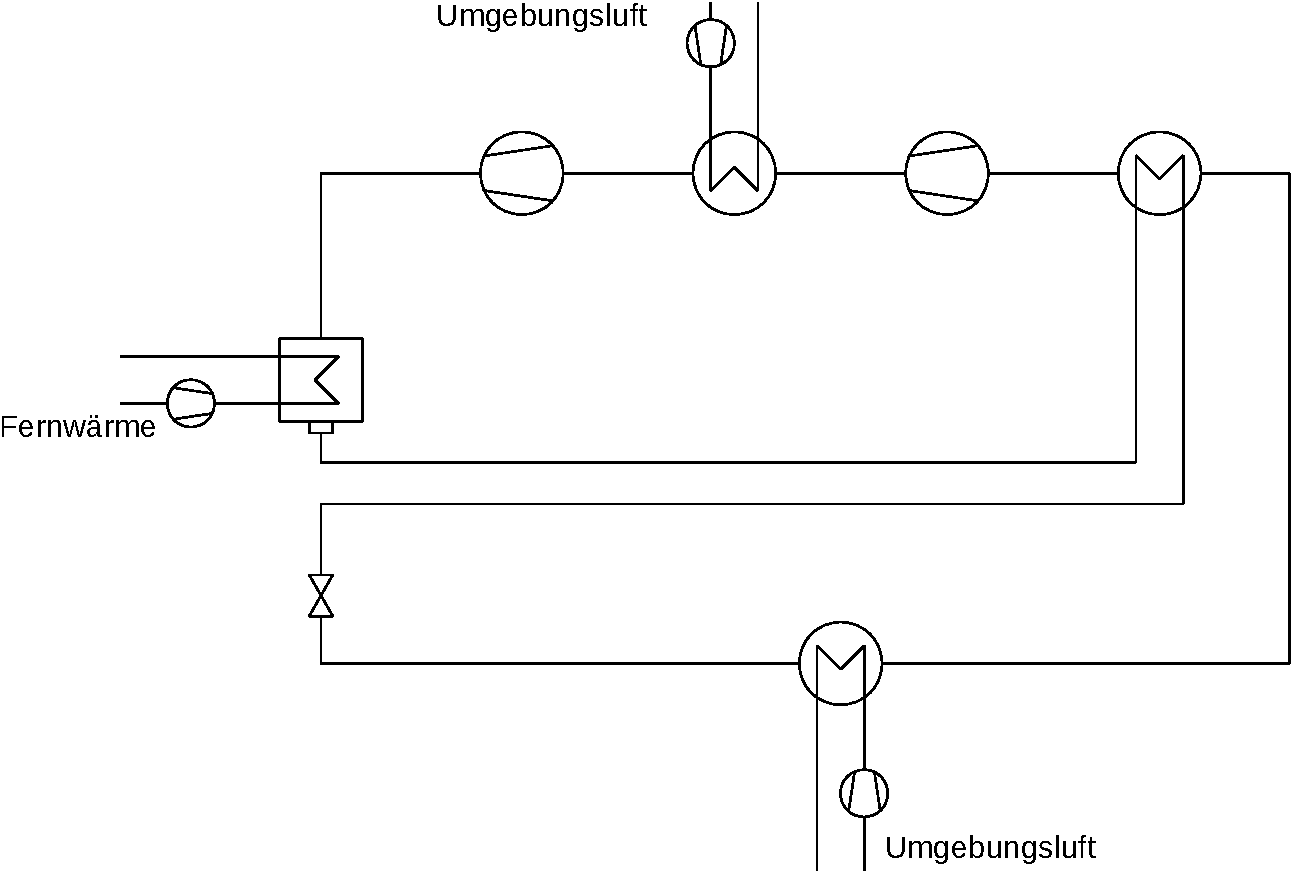
\includegraphics[width=1\textwidth]{Heatpump.pdf}
			\subcaption{Schaltbild}
			\label{subfigure: Schaltbild_Heatpump}
		\end{subfigure}
		\hfill
		\begin{subfigure}[b]{0.48\textwidth}
			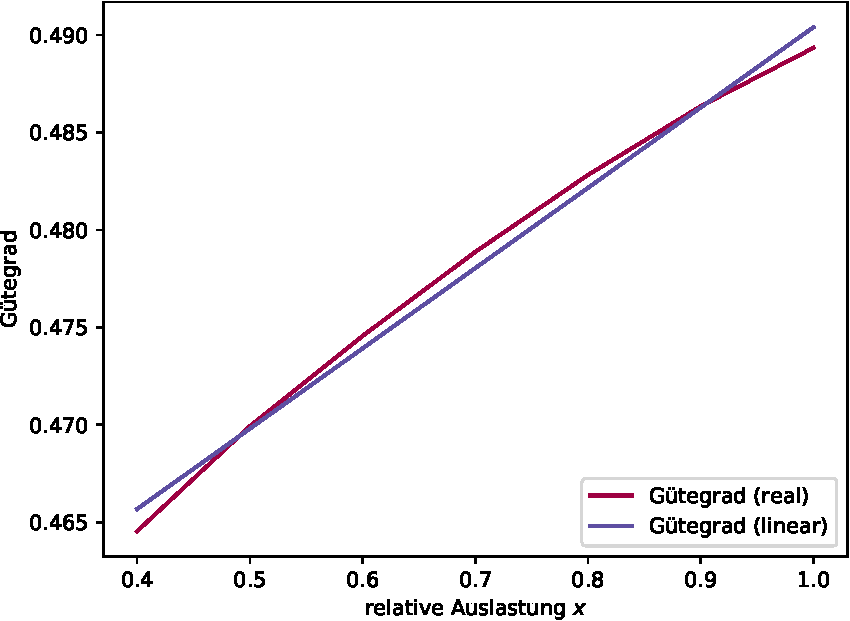
\includegraphics[width=1\textwidth]{Guetegrad_WP.pdf}
			\subcaption{}
			\label{subfigure: Guetegrad_WP}
		\end{subfigure}
		\caption[Konzeptionelle Darstellung zweier Ansätze zur Steigerung der Speicherkapazität durch Verwendung einer Wärmepumpe]{Schaltbild der modellierten Wärmepumpe (a) und Darstellung des Gütegrads über einer variierenden Auslastung (b)}
		\label{fig: HP - Schaltplan und Guetegrad}
	\end{figure}

Zur Bestimmung des Verhaltens der Wärmepumpe ist eine Ammoniak Kompressionswärmepumpe mit einfacher Unterkühlung in \ac{TESPy} abgebildet worden. Diese nutzt die Umgebungsluft als Wärmequelle. Ziel der Simulation ist die Bestimmung des Gütegrads über einem variierenden Lastbereich. Aus den vorliegenden Daten zur Umgebungstemperatur und der Vorlauftemperatur des Netzes sind Durchschnittswerte gebildet worden, für die die Wärmepumpe ausgelegt wurde. Diese Werte sind Tabelle \ref{tab: Randparameter der Wärmepumpe} zu entnehmen.
	\begin{center}
	\captionof{table}{Auslegungsparameter der Wärmepumpe}
	%\renewcommand{\arraystretch}{1}
	\begin{tabular}{lllll}
		\hline 
		Teilprozess & Parameter  & Symbol  & Einheit  & Wert\tabularnewline
		\hline 
		\textbf{Fernwärme} & Vorlauftemperatur  & $T_{\text{VL}}$  & \textdegree C  &  91,12\tabularnewline
		& Rücklauftemperatur  & $T_{\text{RL}}$  & \textdegree C  & 50\tabularnewline
		& Druck  & $p_{\text{FW}}$  & bar  & 10\tabularnewline
		& Wärmeaufnahme & $\dot{Q}_\text{DH}$ & MW & 145 \tabularnewline
		\textbf{Komponenten} & Verdichterwirkungsgrad  & $\eta_{\text{V,WP}}$  & - & 0,8 \tabularnewline
		& Verdichterdruckverhältnis  & $pr_\text{V}$  & - & 3,3 \tabularnewline
		& Druckverlust der Wärmeübertrager  & $pr_\text{WÜ}$  & - & 0,98 \tabularnewline
		& Lüfterwirkungsgrad  & $\eta_{\text{Lü}}$  & - & 0,6 \tabularnewline
		\textbf{Fluidwerte} & Sattdampfdruck  & $p_{\text{SD}}$  & bar & 6 \tabularnewline
		& Temperatur überhitzter Dampf & $T_{\text{ÜD}}$  & \textdegree C & 16 \tabularnewline
		& Eintrittstemperatur Verdichter 2  & $T_{\text{V2}}$  & \textdegree C & 60 \tabularnewline
		& abgegebener Wärmestrom  & $\dot{Q}_\text{WP}$  & MW & 25 \tabularnewline
		\hline 
		\label{tab: Randparameter der Wärmepumpe}  &  &  & \tabularnewline
	\end{tabular}
	\par\end{center}
Der Gütegrad der Wärmepumpe wird als Funktion der Verdichterleistung, aber nicht der Umgebungstemperatur oder Vorlauftemperatur des Netzes angenommen. Bei dieser Vereinfachung wird die Tatsache außer Acht gelassen, dass der Verdichter der Wärmepumpe mit zunehmender Vorlauftemperatur mehr arbeiten muss, um die gewünschte Temperatur überhaupt zu erreichen. Dieser Fehler wird für eine einfachere Beschreibung jedoch akzeptiert. Die gewonnene Kennlinie kann Gleichung \ref{equation: KennlinieHP} entnommen werden, welche den Gütegrad in Abhängigkeit der relativen Auslastung $x$ der Wärmepumpe darstellt. Der Gütegrad wird zusammen mit einem Schaltbild der modellierten Wärmepumpe in Abbildung \ref{fig: HP - Schaltplan und Guetegrad} dargestellt. 
	\begin{equation}\label{equation: KennlinieHP}
		\eta_\text{WP} = \text{0,0412} x + \text{0,4492}
	\end{equation}

Gleichung \ref{equation: Leistungszahl 1} zeigt, wie die Leistungszahl der Wärmepumpe von der Carnot-Leistungszahl und dem Gütegrad abhängt. Zur Verwendung in Solph ist die Carnot-Leistungszahl im preprocessing für jeden Zeitschritt anhand der Umgebungstemperatur und Vorlauftemperatur berechnet worden und wird als Liste an Solph übergeben. Abbildung \ref{fig: Kennfeld_HP} zeigt die möglichen Leistungszahlen während der Optimierung. Je nach Last und Vorlauf- bzw. Umgebungstemperatur kann in dem Diagramm die aus dem Gütegrad und der Carnot-Leistungszahl resultierende Leistungszahl der Wärmepumpe abgelesen werden.

Zur Implementierung in Solph ist die Komponente \textit{OffSetTransformer} verwendet worden, um zu gewährleisten, dass eine minimale Verdichterleistung bei der Optimierung nicht unterschritten werden kann. Das vollständige Modell und alle Randparameter können dem beigefügten Datenträger entnommen werden.

	\begin{figure}[ht]
		\centering
		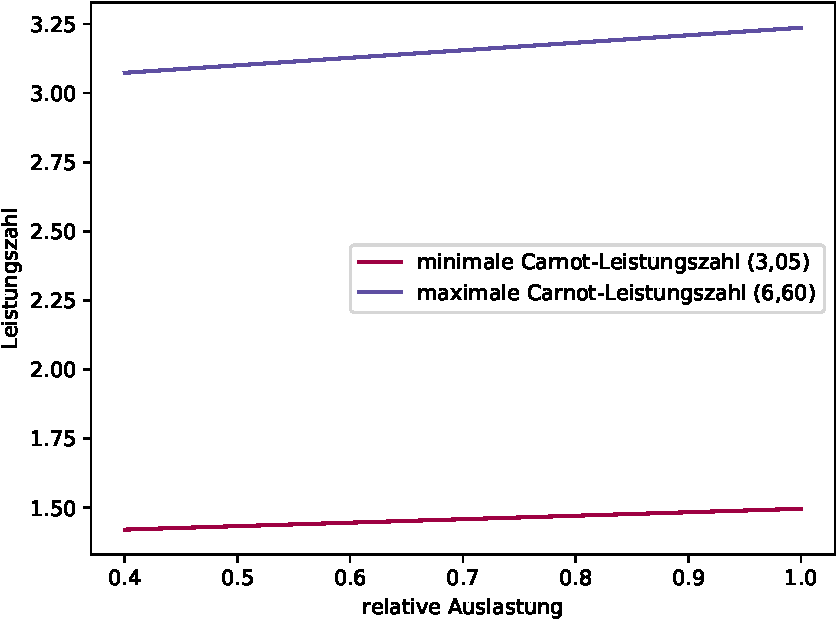
\includegraphics[width=0.8\linewidth]{Kennfeld_HP-cropped.pdf}
		\captionof{figure}[Kennfeld der modellierten Wärmepumpe]{Kennfeld der modellierten Wärmepumpe. Die untere Linie stellt, je nach Auslastung, die minimal mögliche Leistungszahl dar ($\varepsilon_\text{WPC,min}=3,05$) - entsprechend stellt die obere Linie die maximal erreichbare Leistungszahl dar ($\varepsilon_\text{WPC,max}=6,60$). Während der Optimierung operiert die Wärmepumpe stets innerhalb dieser Grenzen.}
		\label{fig: Kennfeld_HP}
	\end{figure}

\section[Sonstige Technologien]{Sonstige Technologien - Wärmespeicher, Elektrodenheizkessel, Spitzenlastkessel und Photovoltaik}
Für Wärmespeicher, Elektrodenheizkessel, Spitzenlastkessel und die \ac{PV}-Anlage sind keine eigenen Simulationen zum Betriebsverhalten durchgeführt worden. Bei jeder dieser Komponenten ist für die Optimierung von einem konstanten Wirkungsgrad ausgegangen worden. Der Wirkungsgrad des Spitzenlastkessel ist über das in Abbildung \ref{fig: Volta-Feuerung} dargestellte Diagramm zur Bestimmung des feuerungstechnischen Wirkungsgrades \cite{Volta2018} abgeschätzt worden. Dargestellt wird der Wirkungsgrad bei variierendem Verbrennungsluftverhältnis über der Rauchgastemperatur. Bei der Abschätzung des Wirkungsgrades ist von einem Verbrennungsluftverhältnis $\lambda = 1$ und gerade keiner Kondensation im Rauchgas (Taupunkt) ausgegangen worden. Der Wirkungsgrad des \acl{EHK} ist einem Übersichtsblatt für verschiedene Erzeugungsanlagen der \textit{Danish Energy Agencey} \cite{Energinet} entnommen.
	\begin{figure}[ht]
		\centering
		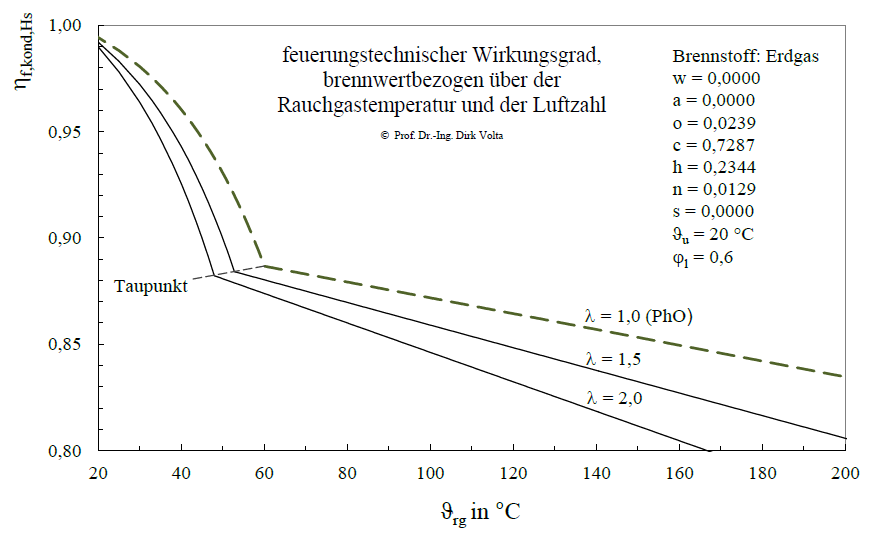
\includegraphics[width=0.8\linewidth]{Volta-Feuerung.png}
		\captionof{figure}[Darstellung des feuerungstechnischen Wirkungsgrads über der Rauchgastemperatur]{Darstellung der Abhängigkeit des feuerungstechnischen Wirkungsgrads über der Rauchgastemperatur für unterschiedliche Verbrennungsluftverhältnisse übernommen aus \cite{Volta2018}}
		\label{fig: Volta-Feuerung}
	\end{figure}

Für die \acl{PV} ist, wie bei der Solarthermie auch, der Anlagen-Ertrag im Preprocessing über Gleichung \ref{equation: LeistungPV} berechnet worden. Der Wirkungsgrad der Module wurde hierbei dem \textit{Photovoltaics Report} \cite{ISE10}, der die durchschnittliche Effizienz von Silizium basierten Modulen mit 17\% angibt, entnommen. Der Wirkungsgrad des Wechselrichters und ein Wert für den Performance Ratio in Deutschland konnten hingegen über \textit{Aktuelle Fakten zur Photovoltaik in Deutschland} \cite{ISE} identifiziert werden. 

Die Wärmespeicher sind als sensible Wärmespeicher angenommen worden. Der entsprechende Wirkungsgrad ist \citet{Kaldemeyer2019} zu entnehmen. In Tabelle \ref{tabelle: Wirkungsgrade Speicher, EHK, SLK und PV} werden alle angenommenen Wirkungsgrade für den Speicher, \acl{EHK}, \acl{SLK} und die \ac{PV}-Anlage aufgelistet. 

	\begin{center}
	\captionof{table}{Wirkungsgrade für Wärmespeicher, Elektrodenheizkessel, Spitzenlastkessel und Photovoltaik}
	\label{tabelle: Wirkungsgrade Speicher, EHK, SLK und PV}
		\begin{tabular}{llclc}
			\hline 
			\rule{0pt}{12pt} Komponente  & Symbol  & Einheit  & Wert & Quelle\tabularnewline
			\hline 
			Wärmespeicher  & $\eta_\text{sp}$  & - & 0,75 & \cite{Kaldemeyer2019}  \tabularnewline
			Elektrodenheizkessel  & $\eta_\text{ehk}$ & - & 0,99 &\cite{Energinet} \tabularnewline
			Spitzenlastkessel  & $\eta_\text{slk}$ & - & 0,88 &\cite{Volta2018} \tabularnewline
			\textbf{Photovoltaik} & & & &\tabularnewline
			Modul  & $\eta_\text{pv}$  & - & 0,17 &\cite{ISE10}  \tabularnewline
			Wechselrichter  & $\eta_\text{wr}$  & - & 0,98 &\cite{ISE}  \tabularnewline
			Performance Ratio  & PR  & - & 0,85 &\cite{ISE}  \tabularnewline
			\hline
		\end{tabular}
	\end{center} 

\chapter{Techno-ökonomische Optimierung}\label{chapter: Techno-ökonomische Betriebsmodelle}
\thispagestyle{empty}
Abbildung \ref{fig: Schema_Optimierung} zeigt das grundsätzliche Vorgehen bei der Optimierung von Energiesystemen. In der Vorbereitung werden die benötigten Daten gesammelt und für die Optimierung entsprechend aufbereitet. Diese Parameter werden dem Modell des Energiesystems als Eingangsdaten zugeführt und innerhalb des Modells genutzt, um entsprechende Randbedingungen für die Einsatzoptimierung zu generieren. Bei der Optimierung wird nun die kostenoptimale Deckung des vorgegebenen Wärmebedarfs bestimmt. Zur Lösung des Optimierungsproblems ist der kommerzielle Solver gurobi \cite{gurobi} verwendet worden, der zu akademischen Zwecken kostenfrei genutzt werden kann. Um die Dauer der Optimierung zu verringern, ist die Genauigkeit des Solvers auf 1\% limitiert worden. Als Ergebnis der Optimierung können beispielsweise die Laufzeiten der Anlagen, der Speicherfüllstand oder der Erlös des Energiesystems ausgelesen werden.
	\begin{figure}[ht]
		\centering
		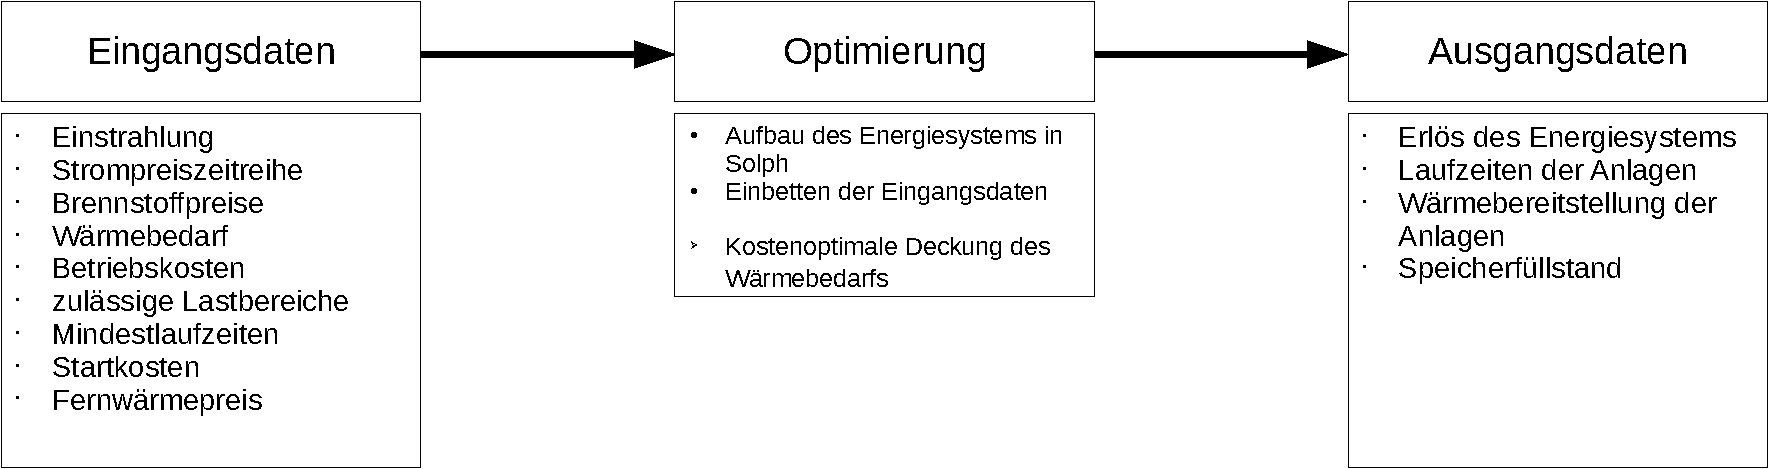
\includegraphics[width=1\linewidth]{Schema_Optimierung.pdf}
		\captionof{figure}{Grundsätzlicher struktureller Aufbau der Betriebsoptimierung}
		\label{fig: Schema_Optimierung}
	\end{figure}

In diesem Kapitel wird gezeigt wie die Konzepte der solarthermischen Wärmebereitstellung in techno-ökonomische Betriebsmodelle überführt worden sind und mit welchem Ergebnis diese Modelle optimiert wurden. Die Ergebnisse der jeweiligen Optimierung werden bewertet und vergleichend in einen größeren Kontext eingeordnet. Zu diesem Zweck wird zunächst die Software Solph vorgestellt, die genutzt worden ist, um die Energiesysteme zu erstellen und zu optimieren. 

Im Anschluss daran werden die Eingangsdaten der durchgeführten Optimierungen genauer betrachtet. In den folgenden Abschnitten wird dann zunächst das Referenzsystem vorgestellt, welches repräsentativ für konventionelle, auf fossilen Brennstoffen basierenden, Wärmeversorgungssysteme in Deutschland stehen soll, bevor die zuvor ausgewählten Alternativsysteme untersucht werden.

\section{Optimierungssoftware Solph}\label{section: Solph}
Solph ist ein Python-Paket des \acf{oemof}, welches vom \citet{RLI2019} und dem \citet{ZNES2019} entwickelt worden ist, um lineare und gemischt-ganzzahlige Probleme zu erstellen und über einen Solver zu lösen. In Solph lassen sich vordefinierte Komponenten miteinander verschalten, um ein Energiesystem aufzubauen. Im Hintergrund wird aus dem erstellten System und den Eingangsdaten die in Kapitel \ref{section: Optimierungsverfahren} beschriebene Zielfunktion und die entsprechenden Nebenbedingungen eines linearen Problems erstellt. Dieses, durch Solph automatisch generierte, lineare Modell wird nun über ein anderes Python-Paket, welches nicht Teil des \acl{oemof} ist, gelöst. Hierbei handelt es sich um Pyomo \cite{hart2017pyomo}, auf das an dieser Stelle nicht weiter eingegangen und auf die entsprechende Dokumentation verwiesen wird. 
	\begin{figure}[ht]
		\centering
		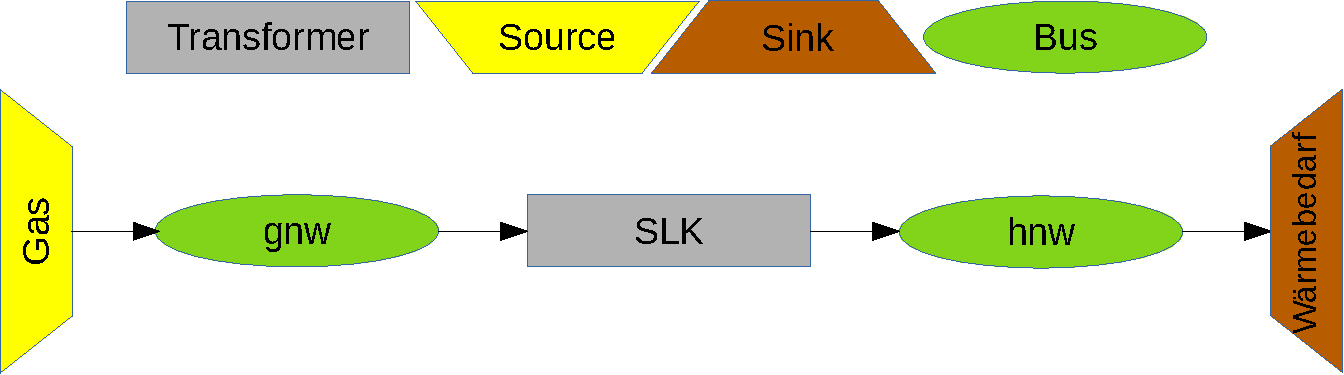
\includegraphics[width=0.8\linewidth]{Solph_Bsp.pdf}
		\captionof{figure}[Schaltlogik eines einfachen Energiesystems in Solph]{Schaltlogik eines einfachen Energiesystems in Solph. Eine Gasquelle ist als Source dargestellt und kann einen Bus, in diesem Fall das Gasnetzwerk (gnw), mit Gas beliefern. Ein Spitzenlastkessel wandelt die Energie des Gases in Wärme um und versorgt das Heiznetzwerk (hnw), aus dem schließlich der Wärmebedarf gedeckt wird.}
		\label{fig: BSP in Solph}
	\end{figure}

In Abbildung \ref{fig: BSP in Solph} wird gezeigt, wie prinzipiell einzelne Anlagen in Solph verschaltet werden können, um ein Energiesystem abzubilden. Dabei stellen Transformer Anlagen dar, die mit einem gewissen Wirkungsgrad (conversion factor) eine oder mehrere Eingangsgrößen transformieren und entsprechende Ausgangsgrößen bereitstellen. Im gezeigten Beispiel ist der \ac{SLK} ein Transformer, der Gas aus dem Gasnetzwerk (gnw) bezieht und die aus dem Gas bezogene Energie in Wärme umwandelt und dem Heiznetzwerk (hnw) zuführt. Aus dem Heiznetzwerk wird nun der Wärmebedarf gedeckt.

Die Verbindungen zwischen den einzelnen Komponenten des Energiesystems werden als Flow bezeichnet und stellen den Energiestrom zwischen verschiedenen Komponenten dar. Je nach Ziel der Optimierung ist es genauso möglich Stoffströme abzubilden, beispielsweise Abgase oder Ware einer Produktion.

Die Flows können mit Kosten oder einem Erlös pro bereitgestellter Einheit belegt werden, so ist es beispielsweise möglich den Flow zwischen der Gas-Source und dem Gasnetzwerk mit einem Gaspreis pro MWh zu belegen. Dieser Wert muss nicht konstant sein. Es können dem Modell auch Preiszeitreihen in stündlicher Auflösung übergeben werden. Dies ist beispielsweise bei dem durch den Börsenhandel volatilen Strompreis der Fall. Zusätzlich können über die Flows variable Betriebskosten der einzelnen Anlagen, maximale bzw. minimale Laufzeiten, eine minimale bzw. maximale Leistung oder Startkosten hinzugefügt werden. Dies sind Parameter aus denen Solph die entsprechenden Randbedingungen für die Optimierung erstellt.

Im folgenden wird kurz gezeigt, wie in Solph ein Energiesystem erstellt werden kann. Diese Betrachtung ist stark an die Solph-Dokumentation \cite{oemof2019} angelegt und für eine genauere Betrachtung wird an eben diese verwiesen. 

Zunächst ist ein Betrachtungszeitraum für die Optimierung erforderlich. Dieser kann über das Python-Paket Pandas erstellt werden. Hier wird, ausgehend von einem Startdatum, der Zeitraum über die Anzahl der Intervalle \textit{periods} und die Schrittweite \textit{freq} (h=Stunden) definiert. In diesem Beispiel ist der Zeitraum 24 Stunden vom 01. Januar 00:00 Uhr:
\begin{lstlisting}[language=python,numbers=none]
import pandas as pd
time_index = pd.date_range('1/1/2016 00:00:00', periods=24, freq='h')
\end{lstlisting}
Dieser Betrachtungszeitraum wird nun genutzt, um ein Energiesystem zu erstellen:
\begin{lstlisting}[language=python,numbers=none]
import oemof.solph as solph
es = solph.EnergySystem(timeindex=time_index)
\end{lstlisting}
Dieses Energiesystem ist leer und enthält nichts weiter als eine Information über den Optimierungszeitraum. In einem nächsten Schritt können dem System nun die gewünschten Komponenten -Bus, Transformer, Source und Sink- hinzugefügt werden:
	\begin{lstlisting}[language=python,numbers=none]
# Source and Sink
gas_source = solph.source(label='gas source',
				outputs={gnw: solph.Flow(variable_costs=1)})
heat_sink = solph.sink(label='heat_sink',
				inputs={hnw: solph.Flow(actual_value=Bedarf, fixed=True)})					   
es.add(gas_source, heat_sink)
		
# Busses
gnw = solph.Bus(label='gas_network')
hnw = solph.Bus(label='heat_network')
es.add(gnw, enw, hnw)
	
# Transformer
SLK = solph.Transformer(label='Spitzenlastkessel',
						inputs={gnw: solph.Flow()},
						outputs={hnw: solph.Flow(nominal_value=30,
											variable_costs=1)},
		  							  conversion_factors={hnw: 0.88})
es.add(SLK)
\end{lstlisting}
In diesem Beispiel ist dem Energiesystem nun eine Gasquelle hinzugefügt worden, aus der bei Bedarf Gas mit einem Preis von 1 pro Einheit bezogen und dem Gasnetzwerk zugeführt wird. An dieser Stelle liegt es an dem Modellierer, welche Einheit die \textit{variable costs} erhalten - es können beispielsweise €/kWh oder €/MWh sein. Die Einheit muss jedoch für das gesamte Modell einheitlich gewählt werden.

Der Spitzenlastkessel bezieht sein Gas aus dem Gasnetzwerk und stellt mit einem Wirkungsgrad von 88\% einen Wärmestrom bereit, der ans Heiznetzwerk abgegeben wird. Der Nenn-Wärmestrom beträgt in diesem Fall 30 - die Einheit ist wieder frei wählbar. Wichtig ist nur, dass die Einheit mit dem Gaspreis zusammenpasst, um plausible Ergebnisse zu erhalten.  
Der Wärmebedarf deckt sich nun aus dem Heiznetzwerk. Durch den Befehl \textit{fixed=True} wird vorgegeben, dass der Bedarf gedeckt sein muss. Das heißt, dass dieser Senke nicht mehr oder weniger Wärme zugeführt werden darf, als benötigt.

Das nun erstellte Netzwerk kann unter Verwendung eines geeigneten Solvers - in diesem Fall des Gurobi-Solvers - gelöst werden:
\begin{lstlisting}[language=python,numbers=none]
model = solph.Model(es)
model.solve(solver="gurobi")
\end{lstlisting}
Im Postprocessing können nun die Ergebnisse der Einsatzoptimierung über weitere Pakete des \acl{oemof} verarbeitet und dargestellt werden.

\section{Eingangsparameter der Optimierung}\label{section: Eingangsparameter der Optimierung}
Die Eingangsparameter der Optimierung können eigene Prognosen oder historische Parameter aus vergangenen Jahren sein. Im Rahmen dieser Arbeit ist das Jahr 2016 als Betrachtungszeitraum gewählt worden, weshalb alle Eingangsdaten aus diesem Zeitraum stammen. Dieser Abschnitt wird die verwendeten Wetterdaten, Preiszeitreihen und Wärmelast kurz vorstellen. Sollten die Daten vor oder nach der Optimierung verwendetet worden sein, wird dieser Abschnitt außerdem erläutern wie dies erfolgt ist. Alle hier aufgeführten Daten können ebenfalls dem beigelegten Datenträger entnommen werden.

Kosten beschreibende Parameter, wie beispielsweise Betriebskosten oder Energiekosten, fließen mit positivem Vorzeichen in die Optimierung ein. Dementsprechend werden alle Parameter, die Einnahmen verursachen - Fernwärmepreise und Stromvermarktung - mit negativem Vorzeichen berücksichtigt.

\subsection*{Wetterdaten}
Für den Betrieb der Solarthermieanlagen sind die standortbezogenen Umgebungsbedingungen entscheidend. Dies sind die Umgebungstemperatur und Sonneneinstrahlung. Die Umgebungstemperatur kann standortspezifisch und unentgeltlich auf der Internetseite Renewables.ninja \cite{pfenninger2016renewables} heruntergeladen werden. Die zugänglichen Daten stellt das MERRA-2 Projekt der Nasa \cite{Gelaro2017a} zur Verfügung. Registrierte Benutzer können die Temperaturen in stündlicher Auflösung für die Jahre 2000 bis 2018 erhalten. Zusätzlich zur Umgebungstemperatur können Daten zu der Bewölkung, der Einstrahlung am Boden und einigen weiteren Parametern abgerufen werden. 

Bei der Sonneneinstrahlung von Renewables.ninja wird jedoch nicht zwischen direkter und diffuser Strahlung unterschieden. Diese Daten lassen sich deshalb nur bedingt weiter verwenden, da bei der Umrechnung von horizontaler in die direkte Einstrahlung Kenntnis über den Diffus-Anteil erforderlich ist. Aus diesem Grund ist für die Einstrahlung ein Datensatz des Deutschen Wetterdienstes verwendet worden. Dieser stellt für ausgewählte Standorte in Deutschland Wetterdaten von 1980 bis 2018 bereit \cite{DWDstrahlung}. Der Standort Schleswig ist repräsentativ für norddeutsche Strahlungsverhältnisse ausgewählt worden.

Die Strahlungsdaten für die horizontale Ebene sind in einem Python-Skript auf eine geneigte Ebene nach dem in Kapitel \ref{Funktionsweise Solarthermische Wärmebereitstellung} vorgestellten DIN-Algorithmus umgerechnet worden. Das Skript ist dem Anhang \ref{Anhang: Sonnenstand} oder dem beigefügten Datenträger zu entnehmen. Die Umgebungstemperatur und Einstrahlung auf die geneigte Ebene sind im Preprocessing genutzt worden, um den Ertrag der Solarthermie zu berechnen. Der so ermittelte, stündlich aufgelöste, Wärmestrom pro m$^2$ wurde schließlich an die Optimierungsmodelle übergeben. Im Fall der Photovoltaik ist ausschließlich die Einstrahlung zur Berechnung der elektrischen Leistung, welche an das Optimierungsmodell übergeben wird, verwendet worden.

\subsection*{Heizlast, Vor- und Rücklauftemperaturen des Wärmenetzes}
Die Stadtwerke Flensburg haben für die Jahre 2014 bis 2016 Daten zu ihrem Fernwärmenetz bereitsgestellt \cite{stadtwerke_flensburg_gmbh_2019_2553968}. Diese beinhalten die Rück- und Vorlauftemperaturen, sowie die Heizlast des Netzes. Diese Daten sind in Bezug auf das Temperaturniveau und den Verlauf der Heizlast als repräsentativ für typische Wärmenetze Norddeutschlands angenommen worden. Die Heizlast ist nach der Einwohnerzahl normiert worden wobei davon ausgegangen wurde, dass die Stadtwerke Flensburg ca. 100.000 Einwohner mit Fernwärme versorgen.

Die größte solarthermische Anlage Deutschlands, mit einer Fläche von 8.300 m$^2$, steht in Senftenberg \cite{SDH2019}. Das Wärmenetz versorgt 25.000 Einwohner und erreicht dabei eine \ac{SF} von 4\% \cite{Senftenberg}. Die Heizlast, die im Rahmen dieser Arbeit zur Optimierung verwendet wird, ist auf eine Einwohnerzahl von ca. 50.000 skaliert worden. Somit wurde die Flensburger Last halbiert. Die Skalierung wurde vor dem Hintergrund gewählt, dass das im Rahmen dieser Arbeit betrachtete Netz größer als bisherige solarthermisch unterstützte Netze in Deutschland ausfallen sollte, aber nicht unrealistisch groß. Prinzipiell kann die Heizlast in Norddeutschland aber auf jede Netzgröße skaliert werden. Abbildung \ref{fig: Heizlast} stellt den Verlauf der gewählten Heizlast grafisch dar. 
	\begin{figure}[ht]
		\centering
		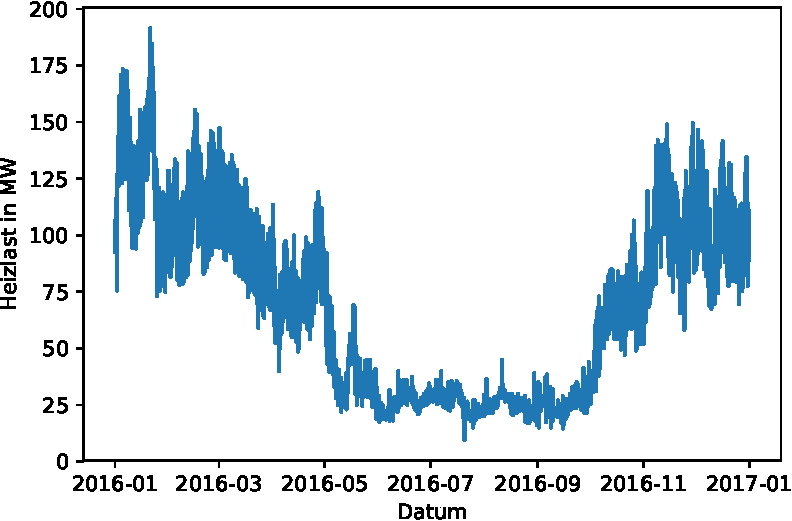
\includegraphics[width=0.8\linewidth]{HL.pdf}
		\captionof{figure}{Darstellung des Verlaufs der Heizlast des untersuchten Wärmenetzes für das Jahr 2016}
		\label{fig: Heizlast}
	\end{figure}

Die Rücklauftemperatur des Netzes wird konstant auf 50\textdegree C gehalten. Die Vorlauftemperatur erreicht im Winter 124\textdegree C und fällt im Sommer auf durchschnittlich 80\textdegree C ab. Diese Temperaturen sind unverändert aus dem Stadtwerke Flensburg Datensatz übernommen und wurden bei der Berechnung des von den Solarkollektoren abgegebenen Wärmestroms genutzt.

\subsection*{Preiszeitreihen Strom, Gas und Fernwärme}
In dieser Arbeit werden folgende Preiszeitreihen benötigt:
	\begin{description}
		\item[Fernwärmepreis] Der Fernwärmepreis ist bei der durchgeführten Optimierung als konstanter Wert angenommen worden. Aus \citet{Kaldemeyer2019} ist ein durchschnittlicher Fernwärmepreis für das Jahr 2016 von 68,59 \euro/MWh übernommen worden.
		\item[Gaspreis] Bei dem Gaspreis wird ebenfalls von einem konstanten Gaspreis über den Betrachtungszeitraum ausgegangen. Die \ac{PEGAS} veröffentlicht den nach Monaten und Jahren aufgeschlüsselten \ac{EGIX} ab dem Jahr 2008. Für die durchgeführte Einsatzoptimierung ist der Durchschnittswert für das Jahr 2016 von 14,14 \euro/MWh verwendet worden. \cite{GasPrice}
		\item[Strompreis (Verkauf)] Im Rahmen dieser Arbeit ist ausschließlich die Stromvermarktung über Day-Ahead Auktionen an der europäischen Strombörse betrachtet worden. Eine stündlich aufgelöste Preiszeitreihe über die Day-Ahead-Strompreise aus dem Jahr 2016 ist dem Agorameter \cite{Agora2016} entnommen worden.
		\item[Strompreis (Bezug)] Der aus dem elektrischen Netz bezogene Strom setzt sich aus der Strompreiszeitreihe für den Verkauf und Stromabgaben\footnote{Stromabgaben setzten sich zusammen aus: EEG-Umlage, Konzessionsabgabe, KWKG-Umlage, §19 StromNEV-Umlage, Offshore-Netzumlage, Stromsteuer} zusammen. Für die Stromabgaben ist ein konstanter Wert von 85,51 \euro/MWh angenommen worden, welcher der Strompreisanalyse des Bundesverbands der Energie- und Wasserwirtschaft \cite{BDEW} entnommen wurde. 
	\end{description} 

\subsection*{Betriebskosten, CO$_2$-Zertifikat, Energiesteuer}
Unter diesem Abschnitt werden alle Kosten, die beim Betrieb der technischen Anlagen anfallen, aufgeführt. Diese reichen von den Betriebskosten, die den Verschleiß und die notwendige Wartung der Anlage berücksichtigen, über CO$_2$-Zertifikatspreise pro t$_{\text{CO}_2}$ zu einer Energiesteuer beim Betrieb eines Spitzenlastkessels. Zunächst sollen die Betriebskosten der Anlagen und ihr Zustandekommen genauer betrachtet werden.
\subsubsection*{Solarthermie / Photovoltaik}
Nach Angaben des Fraunhofer-Instituts für solare Energiesysteme können für den Betrieb von \ac{PV}-Anlagen Kosten in Höhe von 1\% der Investitionskosten angenommen werden \cite{ISE}. Dieser Wert ist für den Betrieb der solarthermischen Anlagen übernommen worden. Die Betriebskosten BK errechnen sich dann über den Quotienten aus dem im Preprocessing ermittelten Ertrag $Q_\text{ST}$ / $W_\text{PV}$ der Anlage und den Investitionskosten $I$. Dies wird in Gleichung \ref{equation: Betriebskosten Solar} und \ref{equation: Betriebskosten PV} veranschaulicht. 
	\begin{align}
		\label{equation: Betriebskosten Solar}
		\text{BK}_\text{ST} &= \dfrac{0,01 \cdot I_\text{ST}}{Q_\text{ST}} \hspace{1cm} [\euro/\text{MWh}]\\
		\label{equation: Betriebskosten PV}
		\text{BK}_\text{PV} &= \dfrac{0,01 \cdot I_\text{PV}}{W_\text{PV}} \hspace{1cm} [\euro/\text{MWh}]
	\end{align}
Die Investitionskosten der Anlagen werden nach den in Kapitel \ref{subsection: Kostendegression} vorgestellten Gleichung ermittelt.

\subsubsection*{Wärmespeicher}
Für den \ac{STES} sind ebenfalls Betriebskosten von 1\% der Investitionskosten angenommen worden, die innerhalb von Solph auf den Input-Flow des entsprechenden Wärmespeichers gelegt wurden. Nach \citet{Waermenetz40} soll es möglich sein den Wärmebedarf eines Netzes für 1/6 des Jahres über den Saisonalen Speicher zu decken. Bei der Referenzwärmemenge zur Bestimmung der Betriebskosten ist die Speicherkapazität versechsfacht worden. Dies ist erfolgt, um zu berücksichtigen, dass durch das Laden und Entladen über den Zeitraum eines ganzen Jahres mehr Wärme als die Speicherkapazität abgegeben wird. Die Berechnung der Betriebskosten des Speicher ist in Gleichung \ref{equation: Betriebskosten STES} festgehalten:
	\begin{equation}
		\label{equation: Betriebskosten STES}
		\text{BK}_\text{STES} = \dfrac{0,01 \cdot I_\text{STES}}{6 \cdot Q_\text{sp}} \hspace{1cm} [\euro/\text{MWh}]
	\end{equation}
Für den Kurzzeitspeicher ist ad hoc ein konstanter Wert von 0,05~\euro/MWh angenommen worden. Die Investitionskosten ergeben sich nach \citet{Waermenetz40} zu 110~\euro/m³. Zusätzlich ist eine Förderung von 30\% der Investitionskosten durch das \citet{BAFA2019} berücksichtigt worden. 

\subsubsection*{Gas- und Dampfkraftwerk}
Nach \citet{Schmitz2009} können die Betriebskosten eines \ac{GuD} zwischen 1,5\% und 3,5\% der Investitionskosten, die sich auf 210-600~\euro/kW$_\text{Kessel}$ belaufen, angenommen werden. Im Rahmen dieser Arbeit ist jeweils mit dem Mittelwert gerechnet worden, womit sich die Investitionskosten der betrachteten Anlage auf ca. 280~Mio.\euro\ belaufen. Außerdem werden die Betriebskosten im Fall der \ac{GuD}-Anlage auf die elektrische Leistung $P$ bezogen. Die gesamte, durch das Kraftwerk bereitgestellte elektrische Energie, ist über eine angenommene Volllaststundenzahl VLH abgeschätzt worden. Nach Angaben der Statista GmbH betrugen die Jahresvolllaststunden eines Braunkohlekraftwerks im Jahr 2017 durchschnittlich 6500\ h \cite{statista2017}. Dieser Wert ist für die betrachtete \ac{GuD}-Anlage übernommen worden, da Braunkohlekraftwerke in der Regel als Grundlastkraftwerke eingesetzt werden und ein ähnlicher Betrieb für das verwendete \ac{GuD} erwartet werden kann. Damit ergeben sich die Betriebskosten nach Gleichung \ref{equation: Betriebskosten GuD} bei einer Nennleistung $P_\text{Nenn}$ von 300~MW und Investitionskosten $I_\text{GuD}$ in Höhe von 281,32~Mio.~\euro\  zu:
	\begin{equation}
		\label{equation: Betriebskosten GuD}
		\text{BK}_\text{GuD} = \dfrac{0,025 \cdot I_\text{GuD}}{P_\text{Nenn} \cdot \text{VLH}} = 3,61 \hspace{1cm} [\euro/\text{MWh}]
	\end{equation}

\subsubsection*{Wärmepumpe, Elektrodenheiz- und Spitzenlastkessel}
Die Kompressionswärmepumpe ist mit konstanten Betriebskosten von 2~\euro/MWh Wärme angenommen worden. Für den Elektrodenheizkessel werden 0,50~\euro/MWh als variable Betriebskosten angesetzt - für den Spitzenlastkessel beläuft sich dieser Wert auf 1 \euro/MWh. Alle Werte stammen aus \textit{Technology Data for Energy Plants for Electricity and District heating generation} \cite{Energinet}.

\subsubsection*{CO$_2$-Zertifikatspreis und Energiesteuer}
Der \citet{BDEW} gibt für das Jahr 2016 einen CO$_2$-Zertifikatpreis von 5,35~\euro/t$_{\text{CO}_2}$. Es ist davon ausgegangen worden, dass bei der Verbrennung von 1~MWh Gas 0,2~Tonnen ${\text{CO}_2}$ freigesetzt werden \cite{Quaschning2015}. Danach ergibt sich der CO$_2$-Zertifikatspreis pro MWh zu:
	\begin{equation*}
		p_{\text{CO}_2} = 5,35 \frac{\euro}{t_{\text{CO}_2}} \cdot 0,2 \dfrac{t_{\text{CO}_2}}{\text{MWh}} = 1,07 \frac{\euro}{\text{MWh}}
	\end{equation*}

In dem Forschungsbericht \textit{Elektrizitätsnetzgekoppelte Fernwärmeversorgung} des Zentrums für nachhaltige Energiesysteme ist für den Spitzenlastkessel eine Energiesteuer von 5,50~\euro/MWh angegeben worden \cite{Kaldemeyer2019}. Dieser Wert ist in dieser Arbeit für den Betrieb des Spitzenlastkessels übernommen worden. Die wichtigsten Eingangsparameter der Optimierung werden in Tabelle \ref{tabelle: Übersicht Energiepreise} zusammengefasst. Es werden keine konkreten Werte für die Betriebskosten der Solarthermie, \ac{PV}-Anlagen oder des \ac{STES} in dieser Tabelle aufgeführt, da diese von der jeweiligen Anlagendimensionierung abhängig sind. Zusätzlich fließen die in Kapitel \ref{chapter: Modellbildung} ermittelten Kennlinien der Technologien in die Optimierung mit ein. Diese werden an dieser Stelle jedoch nicht näher betrachtet.
\newpage
	\begin{center}
		\captionof{table}{Übersicht über die wichtigsten Eingangs- und Randparameter der Einsatzoptimierungen}
		\label{tabelle: Übersicht Energiepreise}
		\begin{tabular}{lllll}
			\hline 
			\rule{0pt}{12pt}& & Einheit  & Wert & Quelle\tabularnewline
			\hline 
			\textbf{Solarthermie / PV} & Einstrahlung (geneigt) $\varnothing$  & kWh/(m$^2$a) & 1169 & \cite{DWDstrahlung} \tabularnewline
			 & Ertrag Solarthermie & kWh/(m$^2$a) & 480 & \tabularnewline
			 & Ertrag Photovoltaik & kWh/(m$^2$a) & 170 & \tabularnewline
		%	&  &  &  &   \tabularnewline
			\textbf{Wärmenetz} & Heizlast $\varnothing$ & MW & 68,07 & \cite{stadtwerke_flensburg_gmbh_2019_2553968}  \tabularnewline
			% &  &  &  &   \tabularnewline
			\textbf{Energiepreise} & Fernwärmepreis  & \euro/MWh & 68,59 & \cite{Kaldemeyer2019}  \tabularnewline
			& Gaspreis  & \euro/MWh & 14,14 & \cite{GasPrice} \tabularnewline
			& Strompreis (Day-Ahead) $\varnothing$ & \euro/MWh & 29 & \cite{Agora2016} \tabularnewline
			& Stromabgaben  & \euro/MWh & 85,51 & \cite{BDEW} \tabularnewline
			% &  &  &  &   \tabularnewline
			\textbf{Betriebskosten} & Kurzzeitspeicher  & \euro/MWh & 0,05 &  \tabularnewline
			& Gas- und Dampfkraftwerk  & \euro/MWh & 3,61 & nach \cite{Schmitz2009} \tabularnewline
			& Wärmepumpe  & \euro/MWh & 2 & \cite{Energinet} \tabularnewline
			& Elektrodenheizkessel  & \euro/MWh & 0,5 & \cite{Energinet} \tabularnewline
			& Spitzenlastkessel  & \euro/MWh & 1 & \cite{Energinet} \tabularnewline
			% &  &  &  &   \tabularnewline
			\textbf{sonstiges} & CO$_2$-Zertifikat  & \euro/MWh & 1,07 & \cite{BDEW} \tabularnewline
			& Energiesteuer  & \euro/MWh & 5,5 & \cite{Kaldemeyer2019} \tabularnewline	
			% &  &  &  &   \tabularnewline
			\textbf{Investionskosten} & \acl{GuD}  & \euro/MW$_\text{Kessel}$ & 405.000 & \cite{Schmitz2009} \tabularnewline
			& \acl{EHK}  & \euro/MW & 60.000 & \cite{Energinet} \tabularnewline		
			& \acl{SLK}  & \euro/MW & 70.000 & \cite{Energinet} \tabularnewline	
			& \acl{WP}  & \euro/MW & 250.000 & \cite{paar2013} \tabularnewline	
			\hline
		\end{tabular}
	\end{center} 


\section{Referenzsystem}
Das Referenzsystem stellt ein auf fossilen Brennstoffen basierendes Wärmeversorgungssystem dar, welches mit ausgewählten solarthermischen Konzepten verglichen wird. In Abbildung \ref{fig: Schema Referenzsystem} wird das Referenzsystem dargestellt, wie es zur Optimierung in Solph implementiert wurde. Es handelt sich hierbei um ein \ac{KWK} dominiertes Wärmesystem, welches den Elektrodenheizkessel und Spitzenlastkessel bei hohen Wärmelasten als Reserve verwenden soll. Bevor im folgenden Abschnitt die Alternativsysteme vorgestellt werden, bei denen es sich um das Referenzsystem und Erweiterungen um die ausgewählten Solarthermie-Konzepte handelt, wird an dieser Stelle zunächst der Aufbau, die Auslegung und Implementierung des Referenzsystems in Solph näher betrachtet.
	\begin{figure}[ht]
		\centering
		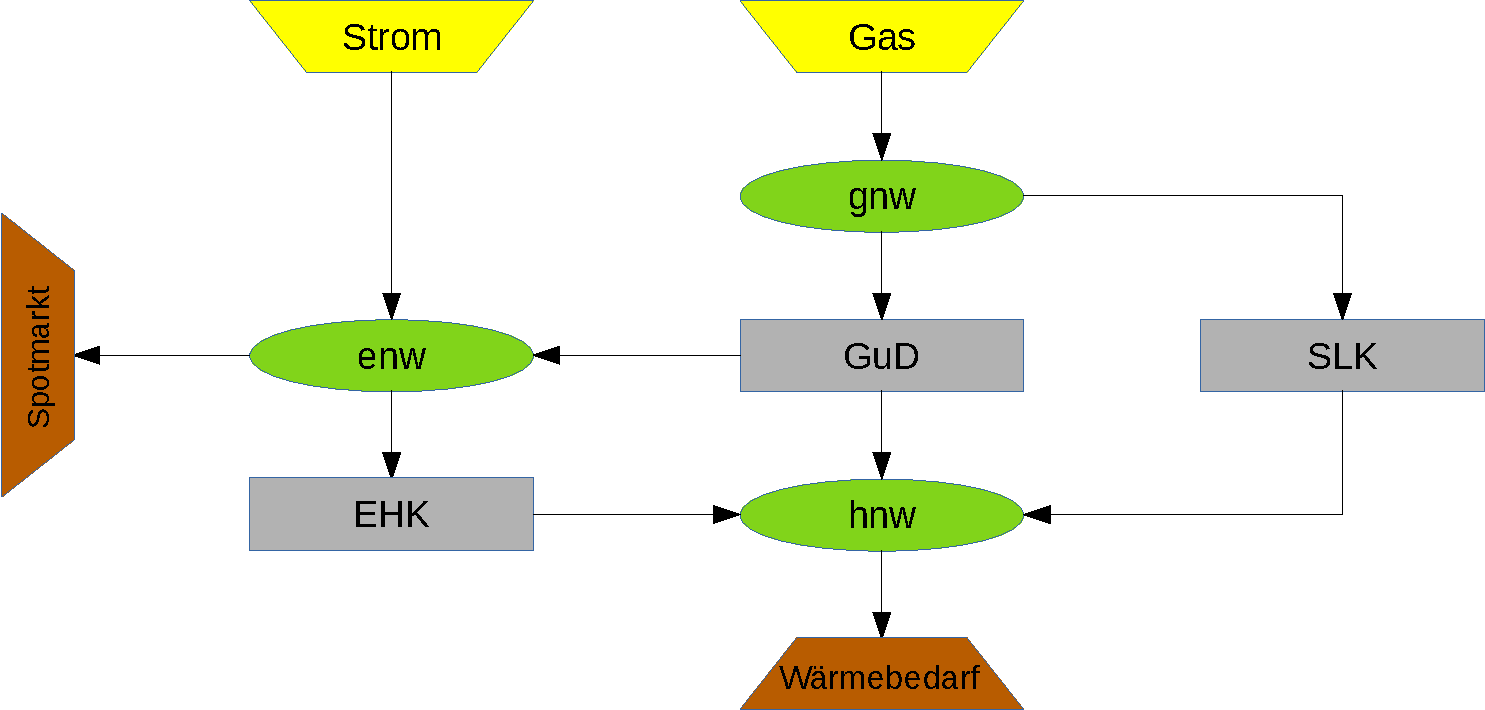
\includegraphics[width=0.8\linewidth]{Solph_Referenzsystem.pdf}
		\captionof{figure}[Schematische Darstellung des in Solph implementierten Referenzsystems]{Schematische Darstellung des in Solph implementierten Referenzsystems. Das benötigte Gas zum Betrieb des \ac{GuD} und \ac{SLK} wird von der Gassource an das Gasnetzwerk (gnw) geliefert. Der \ac{EHK} kann Strom aus dem elektrischen Netz (enw) beziehen, welches aus der Strom-Source und dem \ac{GuD} gespeist wird. Alle Transformer speisen zur Deckung des Wärmebedarfs in das Heiznetzwerk. Bei überschüssiger Stromerzeugung ist eine Vermarktung am Spotmarkt möglich}
		\label{fig: Schema Referenzsystem}
	\end{figure}

Aus dem Datensatz für das Flensburger Fernwärmenetz geht hervor, dass der maximale Wärmebedarf im Jahr 2016 ca. 191,5 MW betrug. Das Referenzsystem ist so dimensioniert, dass eine Reserve von 10 MW vorliegt. Die \ac{GuD}-Anlage soll einen Wärmestrom von bis zu 145 MW liefern. Sowohl der Spitzenlastkessel als auch der Elektrodenheizkessel können maximal 30 MW bereitstellen. Wie in Abbildung \ref{fig: Schema Referenzsystem} zu erkennen ist, beziehen sowohl das \ac{GuD} als auch der \ac{SLK} ihren Brennstoff aus dem Gasnetzwerk (gnw), welches von der Gasquelle gespeist wird. In dem Optimierungsmodell ist der Fluss von der Gasquelle zum Gasnetzwerk mit dem Gaspreis und dem CO$_2$-Zertifikatspreis belegt. Der \ac{EHK} bezieht den elektrischen Strom aus dem eletkrischen Netzwerk (enw) und gibt die Wärme wiederum an das Heiznetzwerk (hnw) ab. Das elektrische Netzwerk wird aus der \ac{GuD}-Anlage und dem eigentlichen Netz versorgt. Der Energiestrom der Strom-Source ist mit der Preiszeitreihe des Day-Ahead-Marktes (im Folgenden Spotmarkt) und den Stromabgaben aus 2016 belegt. Der Energiefluss des \ac{GuD} ist mit den Betriebskosten der Anlage belegt. 

Bei einer Überproduktion an elektrischer Energie kann diese am Spotmarkt zum Preis der Day-Ahead-Auktionen verkauft werden. Hierbei handelt es sich um eine variable Senke, da die Menge an gelieferter Energie nicht festgelegt ist. Im Gegensatz dazu ist der Wärmebedarf an Fernwärme (\ac{DH}) $\dot{Q}^{dh}$ zu jedem Zeitpunkt der Simulation exakt zu decken. Dieser Zusammenhang ist in Gleichung \ref{equation: Bedingung Waermeversorgung} dargestellt:
	\begin{equation}
		\label{equation: Bedingung Waermeversorgung}
		\dot{Q}^{dh} = \dot{Q}_{\text{C}}^{dh} + \dot{Q}_{\text{S}}^{dh} + \dot{Q}_{\text{E}}^{dh}
	\end{equation} 
hierin ist
	\begin{tabbing}
		\hspace{0.5cm}\=\hspace{1cm}\=\hspace{0.5cm}\=\hspace{1cm}\=\kill
		\> $\dot{Q}_{\text{C}}^{dh}$ \>  \>  Wärmestrom des \ac{GuD} an \ac{DH}\\
		\> $\dot{Q}_{\text{S}}^{dh}$ \> \>  Wärmestrom des \ac{SLK} an \ac{DH}\\
		\> $\dot{Q}_{\text{E}}^{dh}$ \> \>  Wärmestrom des \ac{EHK} an \ac{DH}\\
	\end{tabbing} 

Bei der \ac{GuD}-Anlage handelt es sich in Solph um die GenericCHP-Komponente, welche mit den in Kapitel \ref{section: Gas- und Dampfkraftwerk} ermittelten Parametern implementiert worden ist. In Tabelle~\ref{tab: Notwendige Eckdaten zur Verwendung der GenericCHP-Komponente} sind diese Parameter, über die ein zulässiges PQ-Diagramm gebildet wird, bereits aufgeführt worden. Zusätzlich zu diesen Daten ist das \ac{GuD} mit einer Mindest-Standzeit und Startkosten belegt worden, um zu verhindern, dass die Anlage während der Simulation dauerhaft anspringt und nach nur einem Zeitschritt direkt ausgeht. Nach \citet{christidis2011} kann bei einer stündlich aufgelösten Optimierung auf die Modellierung einer Lastrampe beim Start und Stopp des Kraftwerks verzichtet werden. Die Mindest-Standzeit ist mit 5h und die Startkosten mit 4000~$\euro$ in die Simulation eingegangen \cite{christidis2011}. 

Der \ac{EHK} und \ac{SLK} sind als einfache Transformer mit einem konstanten Wirkungsgrad abgebildet worden. Auf eine Mindest-Stillstandzeit und Startkosten wurde bei diesen Komponenten verzichtet. Im Gegensatz zur modellierten \ac{GuD}-Anlage kann der Transformer jeden Betriebspunkt zwischen 0\% und 100\% der Nennleistung  anfahren. Es sind folglich Wärmeströme zwischen 0 und 30~MW von diesen Komponenten zu erwarten. Der \ac{SLK} und \ac{EHK} sind bei der Modellierung möglichst einfach gehalten, um den Simulationsaufwand so weit wie möglich zu reduzieren. 

Ziel der Einsatzoptimierung ist die Minimierung des Betriebsergebnisses, welches, auf Grund der mit negativem Vorzeichen in die Optimierung einfließenden Erlöse für die Fernwärme und Stromvermarktung, negativ ausfällt. Die Zielfunktion, die dieses Modell mathematisch beschreibt, kann Gleichung \ref{equation: Zielfunktion Referenzsystem} entnommen werden:
	\begin{equation}
		\label{equation: Zielfunktion Referenzsystem}
		\text{min }  Z_{Ref} = \text{min} \left[ \sum_{t}^{} \left( (C_{C,t} - R_{C,t}) + (C_{S,t} - R_{S,t}) + (C_{E,t} - R_{E,t}) + C_{CO,t} \right) \right]
	\end{equation}
Sie wird über die Kosten $C$ und Erlöse $R$ der im System verwendeten Technologien gebildet. Wie sich die einzelnen Terme der Zielfunktion zusammensetzen, kann Gleichung \ref{equation: Kosten-GuD} bis \ref{equation: Kosten-CO2} entnommen werden.
	\begin{align}
		\label{equation: Kosten-GuD}
		C_{C,t} &= \dot{Q}_{C,t}^{gas} \cdot  c_{t}^{gas} + P_{C,t} \cdot c_{C,t}^{BK} + Y_{C,t}^{\text{start}} \cdot c_{C,t}^{\text{start}} \\
		R_{C,t} &= \dot{Q}_{C,t}^{dh} \cdot c_t^{dh} + P_{C,t} \cdot c_t^{sm} \\
		C_{S,t} &= \dot{Q}_{S,t}^{gas} \cdot c_{t}^{gas} + \dot{Q}_{S,t}^{dh} \cdot c_{S,t}^{BK} + \dot{Q}_{S,t}^{dh} \cdot c_{S,t}^{es} \\
		R_{S,t} &= \dot{Q}_{S,t}^{dh} \cdot  c_t^{dh} \\
		C_{E,t} &= P_{E,t} \cdot  (c_{t}^{sm} + c_{t}^{sa}) + \dot{Q}_{E,t}^{dh} \cdot c_t^{dh} \\
		R_{E,t} &= \dot{Q}_{E,t}^{dh} \cdot  c_t^{dh} \\
		\label{equation: Kosten-CO2}
		C_{CO2,t} &= \dot{Q}_{gas,t} \cdot  c_{CO2,t}
	\end{align}
Die Kosten des \ac{GuD} $C_{C,t}$ werden über den aufgenommenen Gasstrom $\dot{Q}_{C,t}^{gas}$ und den Gaspreis $c_{t}^{gas}$, die Betriebskosten $c_{C,t}^{BK}$ pro MW elektrischer Leistung $P_{C,t}$ sowie die Startkosten für das Hochfahren der Anlage $c_{C,t}^{\text{start}}$ gebildet. Entsprechend wird der Erlös in Gleichung \ref{equation: Kosten-CO2} über die erzeugte Fernwärme und die vermarktete elektrische Leistung gebildet. Analog werden die anderen Technologien beschrieben. Die Kosten der CO$_2$-Zertifikate werden über den gesamten Gasstrom zum Zeitpunkt $t$ und den Zertifikatspreis $c_{CO2,t}$ abgebildet.
Die Bedeutung der verwendeten Indizes und Abkürzungen kann folgender Auflistung entnommen werden.

	\begin{tabular}{llllll}
		&&&&&  \tabularnewline
		C & \acl{GuD} & es & Energiesteuer & Y & Statusvariable Ein/Aus\tabularnewline
		&&&&& \tabularnewline
		S & \acl{SLK} & BK & Betriebskosten & start & Startbezug\tabularnewline
		&&&&& \tabularnewline
		E & \acl{EHK} & sm & Spotmarkt & $t$ & Zeitschritt \tabularnewline
		&&&&&  \tabularnewline
		&  & sa & Stromabgaben &  & \tabularnewline
	\end{tabular}

\section{Alternativsysteme}
Bei den Alternativsystemen handelt es sich stets um das bereits beschriebene Referenzsystem, welches um die in Kapitel \ref{section: Konzepte} ausgewählten Konzepte der solarthermischen Wärmebereitstellung erweitert wurde. Die Anlagendimensionierung des Referenzsystems hat sich bei der Erweiterung um andere Technologien nicht geändert. Das heißt, dass die mögliche Überproduktion an Wärme im Vergleich zum Referenzsystem steigt. Die Alternativsysteme, welche in den folgenden Abschnitten genauer betrachtet werden, sind mit drei verschiedenen Anlagengrößen für die Solarthermie und den Saisonalen Speicher simuliert worden. Danach ergeben sich für jedes Konzept insgesamt neun verschiedene Setups. Folgende Anlagendimensionierungen wurden betrachtet:

	\begin{tabular}{llllll}
		&&&&&  \tabularnewline
		\textbf{Kollektorfläche:} & 70.000 & \textbf{140.000} & 210.000 & m$^2$  \tabularnewline
		&&&&& \tabularnewline
		\textbf{Speicherkapazität:} & 20.000 & \textbf{60.000} & 100.000 & MWh \tabularnewline
		&&&&& \tabularnewline	
	\end{tabular}

In der Auflistung ist eine Kollektorfläche von 140.000~m$^2$ und eine Speicherkapazität des \ac{STES} von 60 GWh hervorgehoben worden, da diese Auslegungen für die Alternativsysteme als Basis-Szenario festgelegt wurden. Die Kollektorfläche ist vor dem Hintergrund gewählt worden, dass der Solaranlagen-Ertrag am sonnigsten Tag des Jahres (nach vorliegendem Datensatz der 11.06.) gleich dem Wärmebedarf dieses Tages sein soll. Die daraus hervorgehende Fläche von 140.000~m$^2$ liegt nur knapp unter der derzeit größten Anlage in Silkeborg, die eine Fläche von 156.694~m$^2$ aufweist \cite{SDH2019}. Bei der Speichergröße ist die Anlage in Vojens als Vorlage für das Basis-Szenario verwendet worden, welche über ein Speichervolumen von 200.000~m$^3$ verfügt \cite{Arcon2019}. Bei einer maximalen Energiedichte von 300~kWh/m$^3$ \cite{Sterner2017} entspricht dies einer Kapazität von 60~GWh. Das Basis-Szenario dient als Ausgangspunkt für bei der Berechnung der Kostendegression des \ac{STES}.

\subsection{Solarthermie 1}\label{subsection: Solarthermie 1}
Bei dem Solarthermie 1-Konzept (ST1), welches in Abbildung \ref{fig: Solph_Solarthermie_1} dargestellt wird, handelt es sich um das Referenzsystem, welches um eine Solarthermieanlage und einen saisonalen Wärmespeicher erweitert worden ist. Der spezifische Ertrag (MW/m$^2$) der Solaranlage ist im Preprocessing über die DIN EN 12975 und die in Kapitel \ref{section: Modellbildung - Solarthermie} ermittelten Verlustparameter für Kollektorfelder - bestehend aus Vakuumröhrenkollektoren - bestimmt worden. Dieser ist als Datenreihe an das Optimierungsmodell übergeben worden und wird in diesem als Source abgebildet, die direkt mit dem Heiznetzwerk verbunden ist. Je nach Anlagengröße ist dieser Eingang entsprechend skaliert worden. Es ist davon ausgegangen worden, dass durch den \ac{STES} 100\% der solaren Wärme abgenommen werden kann, weshalb die Solar-Source als fixe Eingangsgröße modelliert worden ist. D. h., dass der Ertrag der Solaranlage auf jeden Fall abgenommen werden muss. Dies gilt entsprechend für alle untersuchten Konzepte.
	\begin{figure}[ht]
		\centering
		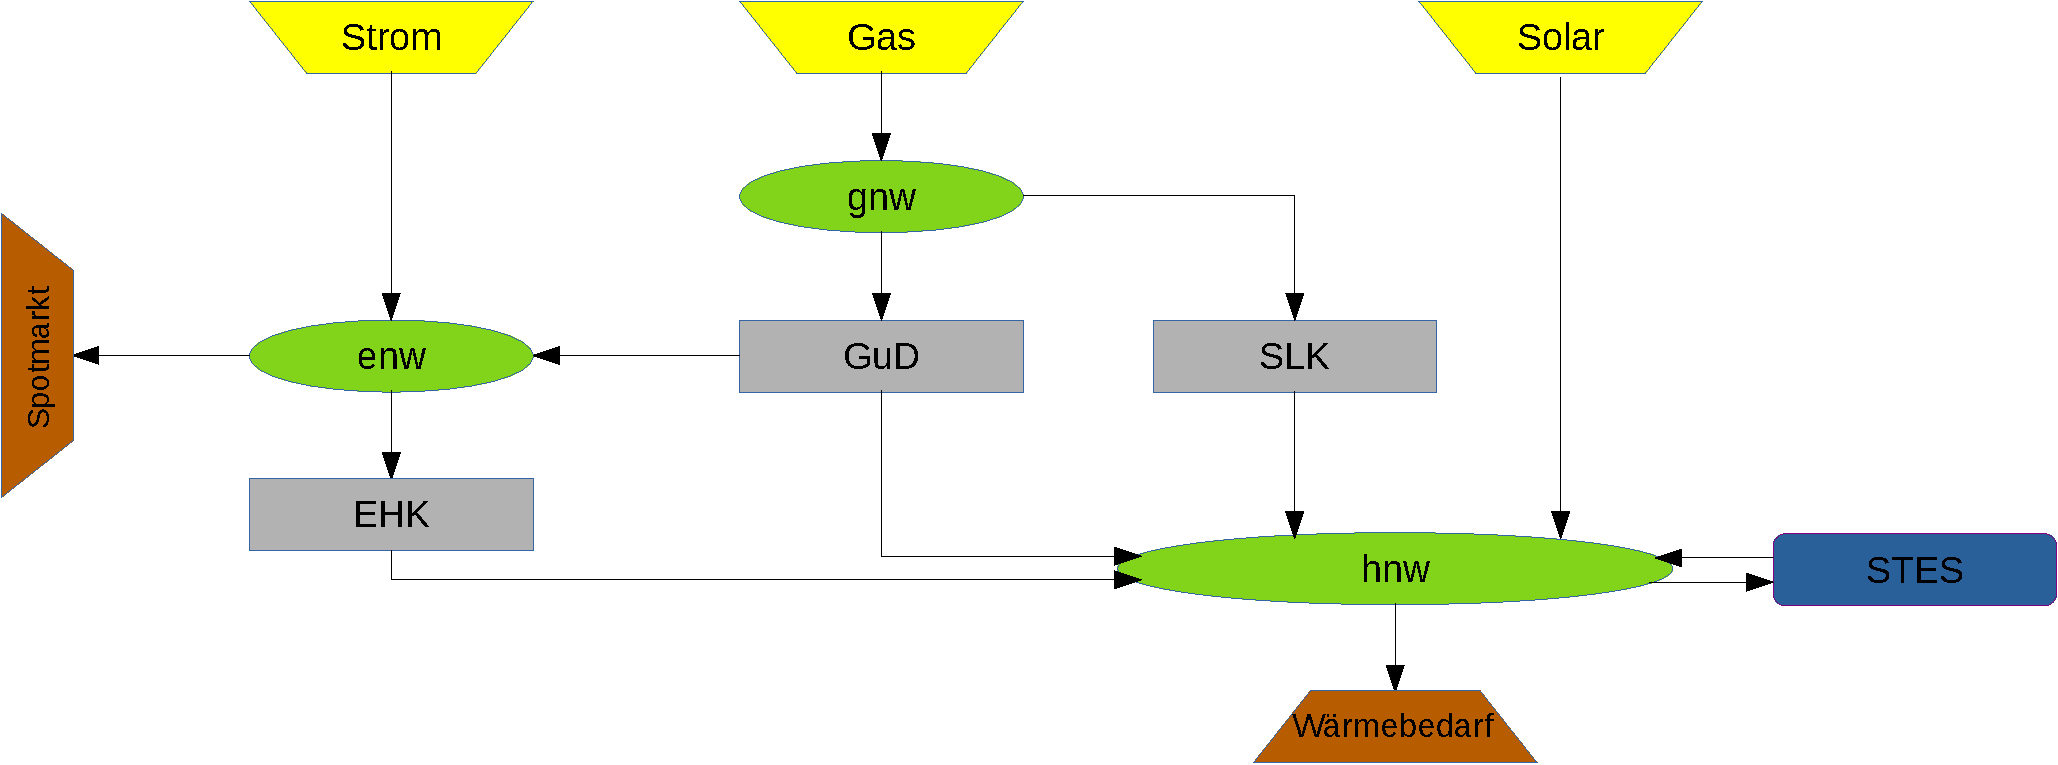
\includegraphics[width=0.8\linewidth]{Solph_Solarthermie_1.pdf}
		\captionof{figure}[Schematische Darstellung des in Solph implementierten Solarthermie 1-Konzepts]{Dargestellt wird eine schematische Darstellung des in Solph implementierten Solarthermie 1-Konzepts. Dabei handelt es sich um das Referenzsystem welches um eine Solar-Source und einen \ac{STES} erweitert worden ist. Der Ertrag aus der Solarthermie ist, wie der \ac{STES} auch, direkt an das hnw angeschlossen.}
		\label{fig: Solph_Solarthermie_1}
	\end{figure}

Tabelle \ref{tabelle: Übersicht flächenspezifische Daten} zeigt, abhängig von der Fläche, den im Preprocessing berechneten Ertrag, die \ac{SF}, Investitionskosten und die Betriebskosten der Solaranlage, welche in der Optimierung mit berücksichtigt werden. Die \ac{SF} stellt hier den maximal möglichen Wert dar, sollte die Wärme aus der Solarthermie ausschließlich direkt genutzt und nicht zwischengespeichert werden, da die Speicherung verlustbehaftet ist. 
	\begin{center}
		\captionof{table}{Übersicht über flächenspezifische Daten der Solarthermie-Anlage}
		\label{tabelle: Übersicht flächenspezifische Daten}
		\begin{tabular}{ccccc}
			\hline 
			Fläche [m$^2$] & Ertrag [MWh] & \ac{SF} [\%] & Investition [\euro]  & Betriebskosten [\euro/MWh] \tabularnewline
			\hline 
			70.000 & 33.331 & 5,57 & 19.135.308 & 5,74 \tabularnewline
			140.000 & 66.622 & 11,14 & 34.327.855 & 5,15 \tabularnewline
			210.000 & 99.933 & 16,71 & 48.032.234 & 4,81 \tabularnewline		
			\hline
		\end{tabular}
	\end{center} 

Der von der Solaranlage übers Jahr maximal abgegebene Wärmestrom ist für den \ac{STES} als höchstmöglicher Wärmeeingang zum Aufladen des Speichers festgelegt worden. Dieser Wert variiert entsprechend der Kollektorfläche. Ein maximaler Entlade-Wärmestrom ist hingegen wesentlich höher angesetzt. Es soll möglich sein, das Wärmenetz zu 100\% aus dem Speicher versorgen zu können, weshalb die Entladung maximal mit der höchstmöglichen Last des Netzes erfolgen kann - in diesem Fall mit 191,5 MW. Darüber hinaus ist der Speicherwirkungsgrad von 75\% auf den abgegebenen Wärmestrom bezogen. Um zu verhindern, dass der Saisonale Speicher wie ein Kurzzeitspeicher genutzt wird, der stündlich aus- und entladen wird, ist der \ac{STES} mit einer minimalen Auflade- und Entladezeit von 3h modelliert worden. Darüber hinaus ist der Speicherstand zu Beginn des betrachteten Zeitraums auf 70\% seiner Kapazität festgelegt. Die kapazitätspezifischen Betriebskosten des Speichers können Tabelle \ref{tabelle: Übersicht kapazitätsspezifische Daten} entnommen werden.
	\begin{center}
		\captionof{table}{Übersicht über kapazitätspezifische Daten des saisonalen thermischen Energiespeichers} 
		\label{tabelle: Übersicht kapazitätsspezifische Daten}
		\begin{tabular}{ccccc}
			\hline 
			Kapazität [GWh] &  &  & Investition (mit Förderung) [\euro]  & Betriebskosten [\euro/MWh] \tabularnewline
			\hline 
			20 &  &  & 7.966.141 & 0.66 \tabularnewline
			60 &  &  & 15.400.000 & 0.43 \tabularnewline
			100 &  &  & 20.923.290 & 0.35 \tabularnewline		
			\hline
		\end{tabular}
	\end{center}

Mathematisch kann die Zielfunktion des ST1-Modells analog zum Referenzsystem beschrieben werden. Sie muss lediglich um einen Term für die Solarthermie-Anlage (ST) und den \ac{STES} erweitert werden. Dies ist in Gleichung \ref{equation: Zielfunktion ST 1} dargestellt.
\begin{equation}
	\label{equation: Zielfunktion ST 1}
	\text{min } Z_{\text{ST1}} = \text{min} \left[Z_{\text{Ref}} +  \sum_{\text{t}}^{} \left((C_{\text{ST,t}} - R_{\text{ST,t}}) + C_{\text{STES,t}} \right)   \right]
\end{equation}
Wie sich die Kosten und der Erlös der Solarthermie-Anlage sowie die Kosten des Speichers bilden, ist Gleichung \ref{equation: Kosten-ST} bis \ref{equation: Kosten_STES} zu entnehmen.
\begin{align}
	\label{equation: Kosten-ST}
	C_{\text{ST,t}} &= \dot{Q}_{\text{ST,t}}^{\text{DH}} \cdot c_{\text{ST,t}}^{\text{BK}} \\
	R_{\text{ST,t}} &= \dot{Q}_{\text{ST,t}}^{\text{DH}} \cdot c_{\text{t}}^{\text{DH}}\\
	\label{equation: Kosten_STES}
	C_{\text{STES,t}} &= \dot{Q}_{\text{STES,t}}^{\text{ein}} \cdot c_{\text{STES,t}}^{\text{BK}}
\end{align}


\subsection{Solarthermie 2}
Abbildung \ref{figure: Solph_Solarthermie_2} zeigt das Solarthermie 2-Konzept (ST2) in der Form, wie es in Solph implementiert worden ist. Es wurden zusätzlich zur solarthermischen Anlage und dem \ac{STES} des ST1-Konzepts eine Wärmepumpe und ein Kurzzeitspeicher hinzugefügt.
	\begin{figure}[ht]
		\centering
		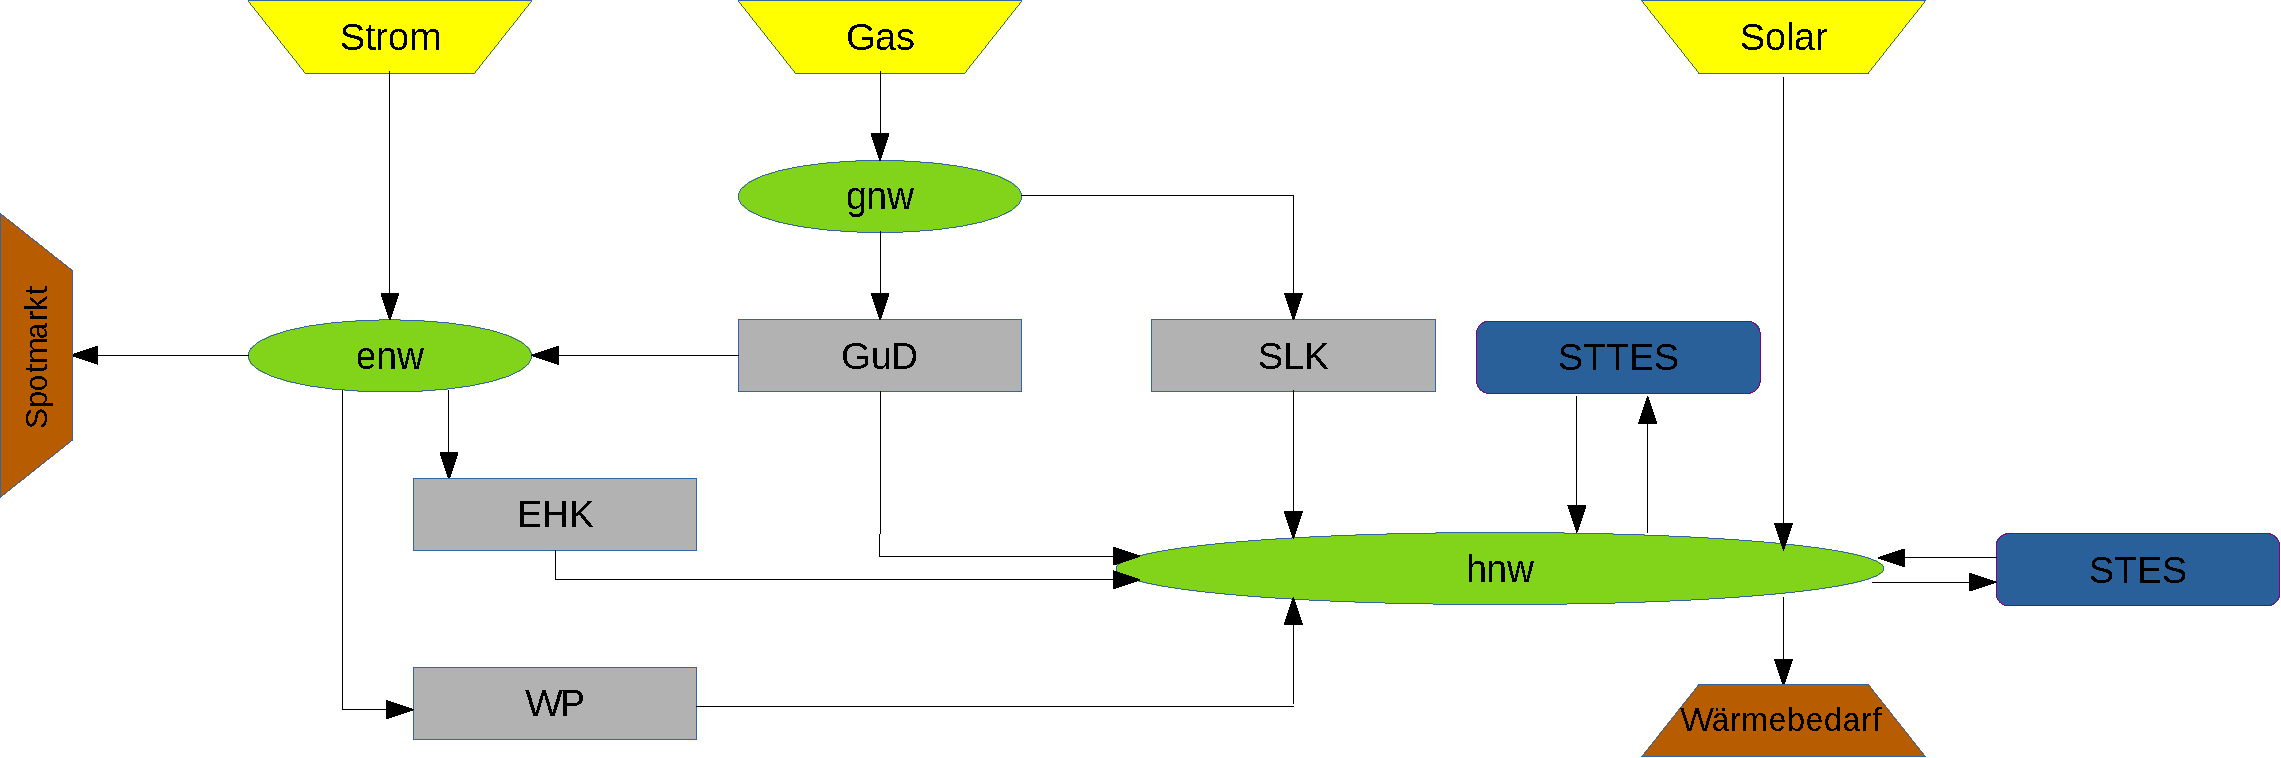
\includegraphics[width=0.8\linewidth]{Solph_Solarthermie_2.pdf}
		\captionof{figure}[Schematische Darstellung des in Solph implementierten Solarthermie 2-Konzepts]{Schematische Darstellung des in Solph implementierten Solarthermie 2-Konzepts. Hierbei handelt es sich um das ST1-Konzept, welches um einen Kurzzeitspeicher und eine Wärmepumpe erweitert wurde. Der Speicher (STTES) ist direkt mit dem hnw verbunden - die Wärmepumpe bezieht den elektrischen Strom aus dem enw und speist die Wärme in hnw.}
		\label{figure: Solph_Solarthermie_2}
	\end{figure}

Die Wärmepumpe ist in Solph als OffsetTransformer modelliert worden. Das heißt, dass die \ac{WP} in dieser Optimierung unter einer Leistung von 40\% ihrer Nennleistung nicht arbeitet. Über die \ac{TESPy}-Simulation einer Wärmepumpe ist, wie in Kapitel \ref{section: Modellbildung - Kompressionswärmepumpe} bereits dargestellt, der Gütegrad über einer variierenden Auslastung ermittelt worden. Dieser ist genutzt worden, um die linearisierte Rampe des OffsetTransformers zu definieren. Zusammen mit der, im Preprocessing ermittelten, Carnot-Leistungszahl, die als Datenreihe an das Optimierungsmodell übergeben wird, ist für jeden Zeitschritt eine Leistungs- und Temperaturabhängigkeit (Umgebung und Vorlauf des Netzes) realisiert worden.

Die Kapazität des Kurzzeitspeichers ist so gewählt worden, dass er theoretisch den Wärmebedarf des Netzes über 6~Stunden decken kann. Bei einem maximalen Bedarf von 191,5~MW entspricht dies einer Kapazität von 1149~MWh. Die Idee hinter der Verwendung des Kurzzeitspeichers ist, den Einsatz der Wärmepumpe zu optimieren - Wärmeproduktion bei niedrigen Strompreisen und zwischenspeichern im Kurzzeitspeicher - ist der maximale Be- und Entladewärmestrom des Speichers auf die \ac{WP} abgestimmt, dessen maximal bereitgestellte Wärme vor der Einsatzoptimierung auf 40~MW abgeschätzt worden ist. Entsprechend wurde dieser Wert für die maximale Be- und Entladung des Speichers übernommen. Im Gegensatz zum \ac{STES} ist beim Kurzzeitspeicher kein Speicherstand zu Beginn der Optimierung vorgegeben worden - dieser ist ein Ergebnis der Einsatzoptimierung. Analog zur \ac{WP} ist die Auslegung des Kurzzeitspeichers Szenario unabhängig. 

Um die mathematische Beschreibung der Zielfunktion des ST2-Konzepts zu erhalten ist die ST1-Funktion um einen Term für die Wärmepumpe und den Kurzzeitspeicher zu erweitern. Dies wird in Gleichung \ref{equation: Zielfunktion ST 2} dargestellt. Gleichung \ref{equation: Kosten-WP} bis \ref{equation: Kosten_STTES} beschreiben dabei die Kosten $C_\text{WP,t}$ und den Erlös $R_\text{WP,t}$ der Wärmepumpe sowie die Kosten des Kurzzeitspeichers $C_{\text{STTES,t}}$.
	\begin{equation}
		\label{equation: Zielfunktion ST 2}
		\text{min } Z_\text{ST2} = \text{min} \left[Z_\text{ST1} + \sum_{\text{t}}^{} ((C_\text{WP,t} - R_\text{WP,t}) + C_\text{STTES,t}) \right]
	\end{equation}
	\begin{align}
		\label{equation: Kosten-WP}
		C_\text{WP,t} &= \dot{Q}_\text{WP,t}^\text{DH} \cdot c_\text{WP,t}^\text{BK} + P_\text{WP,t} (c_\text{t}^\text{sm} + c_\text{t}^\text{sa}) \\
		R_\text{WP,t} &= \dot{Q}_\text{WP,t}^\text{DH} \cdot c_\text{t}^\text{DH}\\
		\label{equation: Kosten_STTES}
		C_{\text{STTES,t}} &= \dot{Q}_{\text{STTES,t}}^{\text{ein}} \cdot c_\text{STTES,t}^\text{BK}
	\end{align}

\subsection{Photovoltaik}
Im Gegensatz zu den vorangegangenen Konzepten, wie in Kapitel \ref{subsection: Konzepte - Photovoltaik und Wärmepumpe} bereits beschrieben, handelt es sich bei diesem Konzept um ein indirektes Solarthermie Konzept bei dem die Wärme nicht direkt von solarthermischen Kollektoren bereitgestellt wird. Zunächst stellen \ac{PV}-Module dem enw elektrischen Strom zur Verfügung, welcher von Wärmepumpen zur Wärmebereitstellung genutzt werden kann. Darüber hinaus ist es jedoch auch möglich den gewonnen \ac{PV}-Strom direkt am Spotmarkt zu vermarkten. Ebenso kann die Wärmepumpe betrieben werden, wenn keine Sonneneinstrahlung vorhanden ist - in diesem Fall wird sie über das \ac{GuD} oder aus dem Strommarkt versorgt. Das in Solph modellierte Energiesystem kann Abbildung \ref{figure: Solph_Photovoltaik} entnommen werden.
	\begin{figure}[ht]
		\centering
		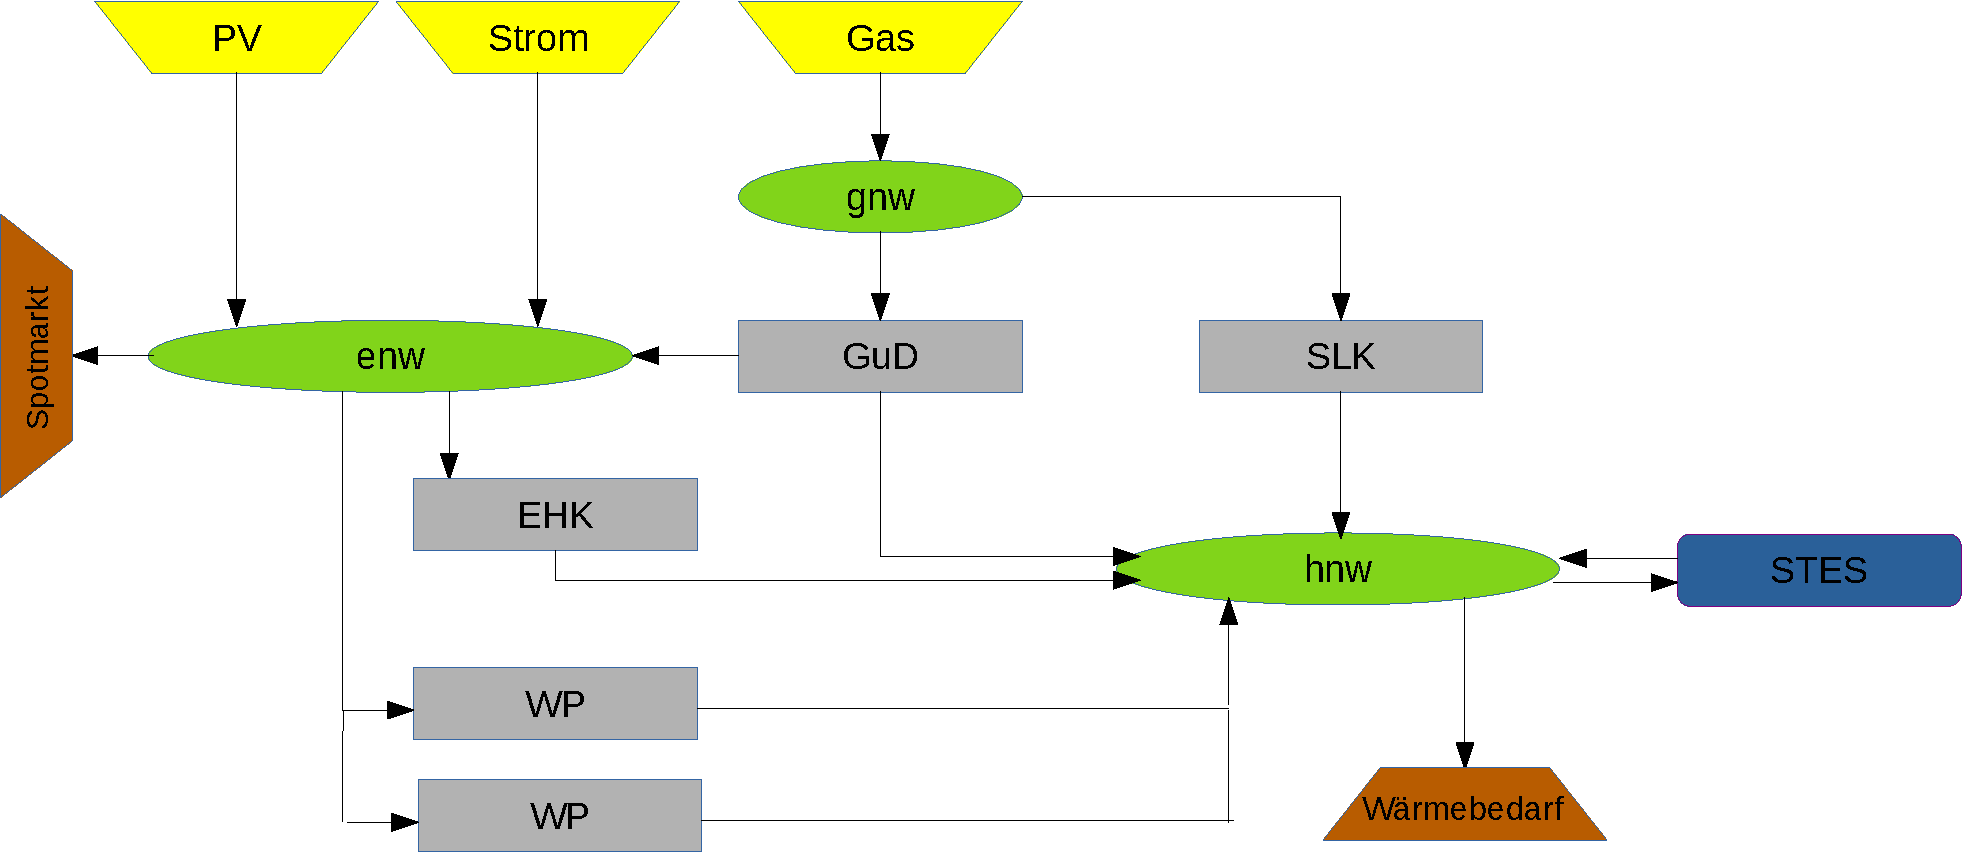
\includegraphics[width=0.8\linewidth]{Solph_Photovoltaik.pdf}
		\captionof{figure}[Schematische Darstellung des in Solph modellierten Photovoltaik-Konzepts]{Schematische Darstellung des in Solph modellierten Photovoltaik-Konzepts. Die von der \ac{PV}-Anlage bereitgestellte elektrische Leistung wird direkt ans enw geliefert, an das auch die beiden Wärmepumpen angeschlossen sind, die den \ac{PV}-Strom zu Bereitstellung von Wärme nutzen können.}
		\label{figure: Solph_Photovoltaik}
	\end{figure}

Der spezifische Ertrag der \ac{PV}-Module ist im Preprocessing über Gleichung \ref{equation: LeistungPV} bestimmt worden und wird als Datenreihe an das Optimierungsmodell übergeben. In dem Modell wird der \ac{PV}-Strom als Source abgebildet und ist an das enw angeschlossen. Entsprechend des Szenarios ist dieser Eingang skaliert worden. Tabelle \ref{tabelle: Übersicht flächenspezifische Daten PV} kann abhängig von dem betrachteten Szenario der Ertrag, die Investitionskosten und Betriebskosten der \ac{PV}-Anlage entnommen werden. 
	\begin{center}
		\captionof{table}{Übersicht über flächenspezifische Daten des Photovoltaik-Konzepts}
		\label{tabelle: Übersicht flächenspezifische Daten PV}
		\begin{tabular}{ccccc}
			\hline 
			Fläche [m$^2$] & Ertrag [MWh] & & Investition [\euro]  & Betriebskosten [\euro/MWh] \tabularnewline
			\hline 
			70.000 & 11.591 & & 11.101.514 & 9,58 \tabularnewline
			140.000 & 23.181 & & 16.826.748 & 7,26 \tabularnewline
			210.000 & 99.933 & & 21.461.247 & 6,17 \tabularnewline		
			\hline
		\end{tabular}
	\end{center} 

Um mit Sicherheit 100\% des \ac{PV}-Stroms in Wärme umwandeln zu können sind zwei Wärmepumpen, die identisch zu der bereits im ST2-Konzept beschriebenen \ac{WP} sind, verwendet worden - diese Anzahl bleibt in jedem Szenario gleich. 
Der \ac{STES} unterscheidet sich in der Modellierung ebenfalls nicht von den vorangegangenen Szenarien. Dementsprechend kann eine genauere Beschreibung der Speicher-Modellierung sowie die von der Kapazität abhängigen Betriebskosten Kapitel \ref{subsection: Solarthermie 1} entnommen werden. 

Die Zielfunktion des Photovoltaik Konzepts ist durch Ergänzung der Referenzsystem-Funktion mit Termen für die \ac{PV}-Anlage, die \ac{WP} und den \ac{STES} zu erhalten - dargestellt in Gleichung \ref{equation: Zielfunktion PV}. Aufgrund der Tatsache, dass in diesem Konzept mehrere Wärmepumpen verwendet werden, sind die Kosten hierfür in allgemeiner Form für eine beliebige Anzahl formuliert worden.
	\begin{equation}
		\label{equation: Zielfunktion PV}
			\text{min } Z_\text{PV} = \text{min} \left[Z_\text{Ref} + \sum_{\text{t}}^{} \left( \sum_\text{\text{WP}}^{} (C_\text{WP,t} - R_\text{WP,t}) + (C_\text{PV,t} - R_\text{PV,t}) + C_\text{STES,t}  \right)     \right]
	\end{equation}

In Gleichung \ref{equation: WP-PV} bis \ref{equation: ErlösPV} wird gezeigt wie sich die einzelnen Terme zusammensetzen. Die Kosten der \ac{WP} bilden sich beispielsweise über den abgegebenen Wärmestrom und die Betriebskosten sowie über die elektrische Leistung und die Summe aus dem Strompreis und den Stromabgaben. 
	\begin{align}
		\label{equation: WP-PV}
		C_\text{WP,t} &= \dot{Q}_\text{WP,t}^\text{DH} \cdot c_\text{WP,t}^\text{BK} + P_\text{WP,t} (c_\text{t}^\text{sm} + c_\text{t}^\text{sa})\\
		R_\text{WP,t} &= \dot{Q}_\text{WP,t}^\text{DH} \cdot c_\text{t}^\text{DH}\\
		C_\text{PV,t} &= \dot{P}_\text{PV,t}^\text{sm} \cdot c_\text{PV,t}^\text{BK} \\
		\label{equation: ErlösPV}\text{}
		R_\text{PV,t} &= \dot{P}_\text{PV,t}^\text{sm} \cdot c_\text{t}^\text{sm}
	\end{align}


\section{Ergebnisse der Einsatzoptimierung}
Nach der Vorstellung aller betrachteten Konzepte in den vorangegangenen Abschnitten wird dieser Abschnitt die Ergebnisse der Einsatzoptimierungen, die mit dem Ziel der Erlös-Optimierung durchgeführt worden sind, für das Referenzsystem und die Alternativsysteme vorstellen. Dabei steht zunächst die Frage im Vordergrund, wie wirtschaftlich die verschiedenen Konzepte und Szenarien im Vergleich zum Referenzsystem sind. Zu diesem Zweck ist vorerst der Kapitalwert genutzt worden. Für die jeweils aussichtsreichsten Auslegungen werden genauere Untersuchung des Betriebsverhaltens der einzelnen Komponenten durchgeführt.

\subsection{Ergebnis der Einsatzoptimierung des Referenzsystems} 
Das Referenzsystem dient als Vergleich zu den erstellten Solarthermie-Systemen und wird zur ökonomischen Bewertung der untersuchten Alternativsysteme herangezogen. Die Einsatzoptimierung des Referenzsystems hat einen, beim optimalen Betrieb der Anlagen, möglichen Erlös von 44,38~Mio.~\euro/a ergeben. Dieser Erlös setzt sich aus der Differenz zwischen den Kosten zum Betrieb der Anlage und Einnahmen durch den Verkauf von Strom und Wärme zusammen. Insgesamt konnte durch die Bereitstellung von Wärme ein Betrag von 41,04~Mio.~\euro\ eingenommen werden. Dieser Wert ist aufgrund eines konstanten Wärmepreises und des gleichbleibenden Wärmebedarfs bei jedem Konzept/Szenario identisch. Die Einnahmen aus dem Verkauf von Strom am Spotmarkt belaufen sich auf 73,9~Mio.~\euro\ und sind damit knapp 80\% größer als die Einnahmen durch den Verkauf von Wärme. Der Kapitalwert des Referenzsystems beträgt, bei einer angenommenen Laufzeit von 20 Jahren und einer Verzinsung von 5\%, insgesamt 267,57~Mio.~\euro. Die Kapitalwerte der Alternativsysteme werden auf diesen Referenz-Kapitalwert bezogen und zeigen somit bei positiven Werten an, dass das Konzept wirtschaftlich attraktiver ist, als das einfache Referenzsystem. Entsprechend zeigen negative Kapitalwerte (bezogen auf das Referenzsystem) an, dass es wirtschaftlicher ist, das Referenzkonzept zu betreiben, ohne die Einbringung von Solarthermie.

	\begin{figure}[ht]
		\centering
		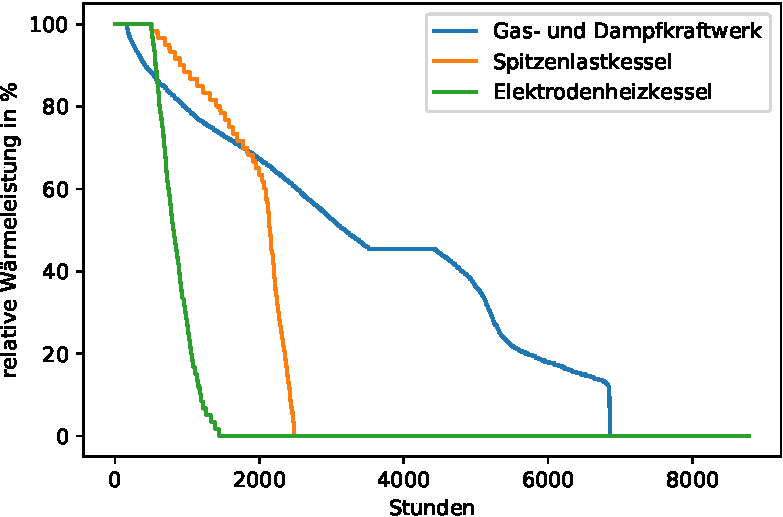
\includegraphics[width=0.8\linewidth]{Jahresdauerlinie_Referenzsystem-cropped.pdf}
		\captionof{figure}[Jahresdauerlinien des Referenzsystems]{Jahresdauerlinien der Wärmebereitstellung aller verwendeten Technologien innerhalb des Referenzsystems. Auf der Abszisse sind die Stunden des Jahres aufgetragen - die Ordinate zeigt die relative Wärmeleistung.}
		\label{figure: Jahresdauerlinien_Referenzsystem}
	\end{figure}

Um das Anlagenverhalten zwischen den Konzepten besser vergleichen zu können ist eine Darstellung des Betriebes in Jahresdauerlinien gewählt worden. Dieser Darstellungsform ist direkt, unabhängig von der entsprechenden Leistung, zu entnehmen, wie eine Anlage über das Jahr betrieben worden ist. Der abgegebene Wärmestrom der Anlage wird in dieser Darstellung auf den über das betrachtete Jahr maximal auftretenden Wärmestrom bezogen. Somit lässt sich Abbildung \ref{figure: Jahresdauerlinien_Referenzsystem} direkt entnehmen, wie viele Stunden die Anlage betrieben worden ist und wie groß der Teillast-Anteil ist.

Es ist zu erkennen, dass die \ac{GuD}-Anlage mit 6850~Betriebsstunden die bevorzugte Technologie zur Wärmebereitstellung darstellt. Es ist aber auch zu erkennen, dass das \ac{GuD} in diesem System nur für wenige Stunden im Jahr ihren vollen Wärmestrom abgibt und quasi dauerhaft in Teillast Wärme bereitstellt. Das heißt jedoch nicht, dass das \ac{GuD} generell in Teillast betrieben wird, da das modellierte Kraftwerk 2 Freiheitsgrade und die Bereitstellung von Wärme und Strom somit entkoppelt sind. Bezogen auf die abgegebene elektrische Energie erreicht das Kraftwerk eine Volllaststundenzahl für den betrachteten Zeitraum von 5371~h. 

Bei dem Betrieb des \ac{EHK} und \ac{SLK} ist zu erkennen, dass diese mit knapp 1500 und 2500~Betriebsstunden deutlich weniger genutzt werden als die \ac{GuD}-Anlage. Beide Anlagen werden unter Volllast über ungefähr den gleichen Zeitraum  verwendet. Die Jahresdauerlinie des Elektrodenheizkessels fällt im Vergleich zum Spitzenlastkessel jedoch stark ab - im niedrigen Leistungsbereich wird der \ac{EHK} nur wenig genutzt. Hervorgehoben wird in Abbildung \ref{figure: Jahresdauerlinien_Referenzsystem} die Bedeutung des \ac{SLK} in dem Referenzsystem. Nach dem \ac{GuD} ist der \ac{EHK} deutlich häufiger und mit einer höheren Auslastung als der \ac{EHK} verwendet worden. Überwiegend ist der Spitzenlastkessel in einem Leistungsbereich zwischen 60\% und 100\% eingesetzt worden. Insgesamt werden im Referenzsystem 86,15\% des Wärmebedarfs von dem \ac{GuD} gedeckt. Der \ac{SLK} stellt 9,6\% und der \ac{EHK} 4,25\% des gesamten Wärmebedarf zur Verfügung. Diese Zahlen heben noch einmal deutlich die Rolle der \ac{GuD}-Anlage im Referenzsystem hervor. 

Die Wärmegestehungskosten des Referenzsystems werden nach Gleichung \ref{equation: vereinfacht Wärmegestehung} berechnet und betragen 32,7 \euro/MWh. Dieser Wert liegt ungefähr in der selben Größenordnung der Wärmegestehungskosten eines auf fossilen Energieträgern basierten Konzepts, bestehend aus einem Blockheizkraftwerk, einer Gegendruckturbine sowie einem Spitzenlast- und Elektrodenheizkessel, welches von \citet{Kaldemeyer2019} untersucht worden ist. Das Ergebnis der Optimierung wird somit als plausibel angesehen.

\subsection{Ergebnisse der Einsatzoptimierung der Alternativsysteme}
An dieser Stelle wird zunächst entschieden, welche Szenarien der einzelnen Konzepte genauer untersucht werden sollen. Als Entscheidungsvariable wird an dieser Stelle der Kapitalwert verwendet. Er wird über die Differenz des Betriebsergebnisses der Alternativkonzepte und dem Ergebnis des Referenzsystems gebildet. In Anlehnung an Gleichung \ref{equation: Kapitalwert-vereinfact} wird die Differenz zwischen den Einnahmen und Ausgaben $(E - A)$ nach Gleichung \ref{equation: E-A} berechnet. Die Investitionskosten beziehen sich bei dieser Rechnung auf die Investitionen, welche das Referenzsystem erweitern.
	\begin{equation}
	\label{equation: E-A}
		(E - A) = (E - A)_\text{Alternativsystem} - (E - A)_\text{Referenzsystem}
	\end{equation}

Abbildung \ref{fig: Heatmaps Solarthermie} und \ref{figure: Heatmap Photovoltaik} zeigen die Ergebnisse der Kapitalwertberechnung für die beiden Solarthermie-Konzepte und das Photovoltaik-Konzept in Form einer Heatmap. Darin werden die Szenarien mit hohen Kapitalwerten dunkel und diejenigen mit niedrigen Werten hell eingefärbt. Diese Heatmaps werden in diesem Abschnitt genutzt, um die Ergebnisse der unterschiedlichen Szenarien zu bewerten.
	\begin{figure}
		\begin{subfigure}[b]{0.48\textwidth}
			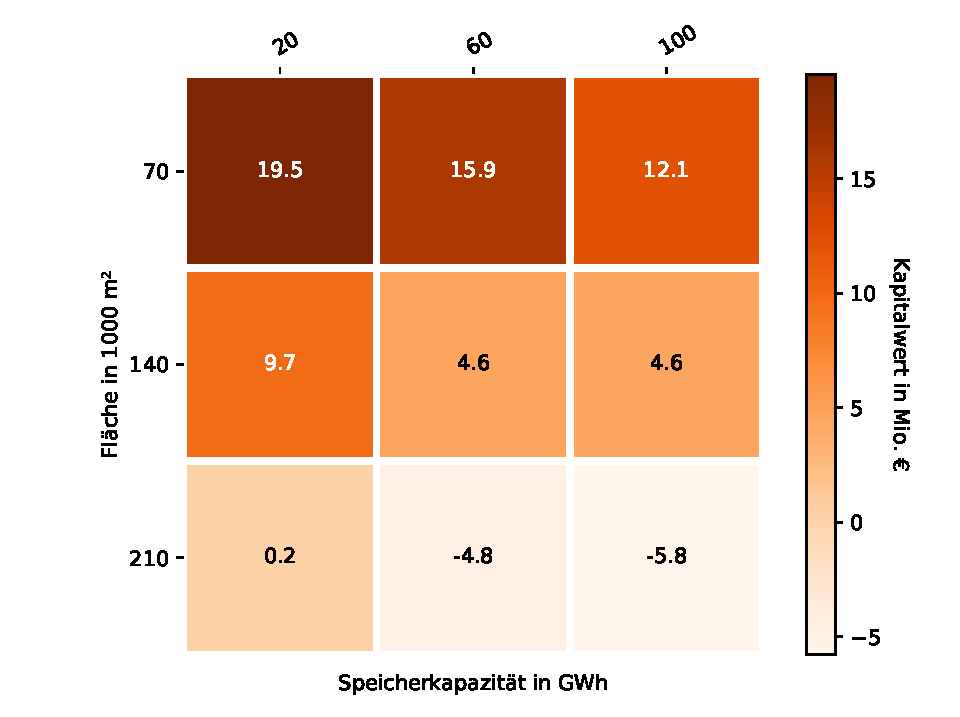
\includegraphics[width=1\textwidth]{Verbesserung/Solar1_Heatmap_relNPV-cropped.pdf}
			\subcaption{Solarthermie 1}
			\label{fig: Heatmaps Solarthermie a}
		\end{subfigure}
		\hfill
		\begin{subfigure}[b]{0.48\textwidth}
			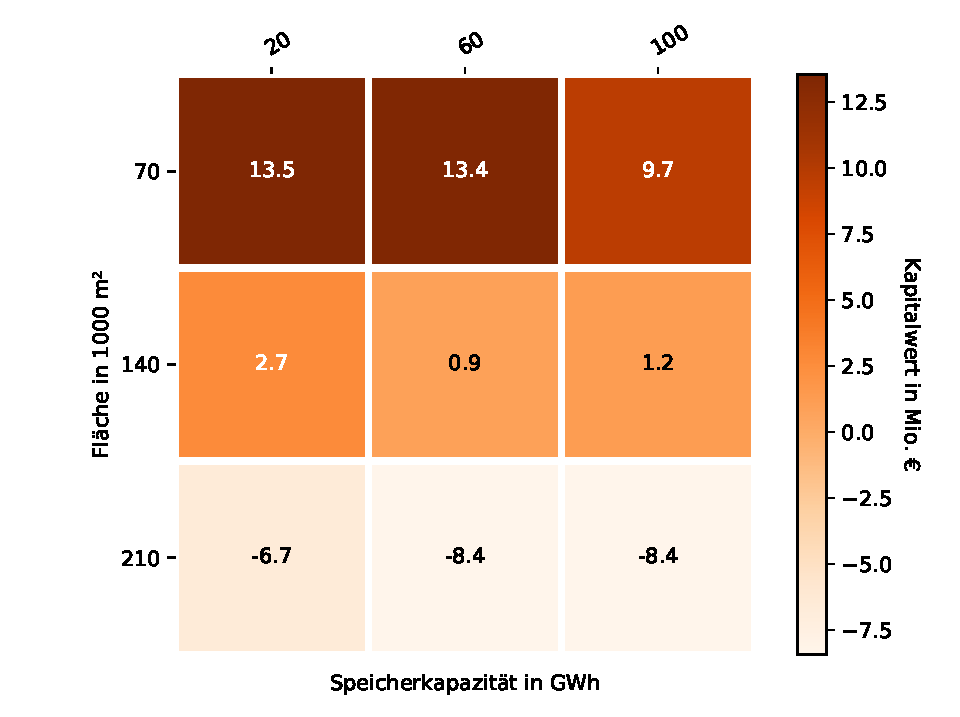
\includegraphics[width=1\textwidth]{Verbesserung/Solar2_Heatmap_relNPV-cropped.pdf}
			\subcaption{Solarthermie 2}
			\label{fig: Heatmaps Solarthermie b}
		\end{subfigure}
		\caption[Übersicht über die Kapitalwerte der Solarthermie Konzepte]{Übersicht über die Kapitalwerte des Solarthermie 1 (a) und Solarthermie 2-Konzepts (b) sowie aller betrachteten Szenarien in Form von Heatmaps. Dunkel dargestellte Flächen zeigen einen höheren Kapitalwert gegenüber den helleren Flächen an.}
		\label{fig: Heatmaps Solarthermie}
	\end{figure}

Wie die Abbildungen \ref{fig: Heatmaps Solarthermie} und \ref{figure: Heatmap Photovoltaik} zeigen, haben alle Konzepte gemeinsam, dass das wirtschaftlich attraktivste Szenario stets jenes mit der niedrigsten Kollektorfläche und geringsten Speicherkapazität ist. Bei dem Solarthermie~1 und Solarthermie~2 Konzept sorgen zunehmende Dimensionierungen der Anlagen dafür, dass der Kapitalwert negative Werte annimmt. Das bedeutet, dass der Betrieb dieser Szenarien, im Vergleich zum Referenzkonzept, unwirtschaftlich ist. Bei dem ST1-Konzept ist dies erst bei einer Kollektorfläche von 210.000~m² und einer Speicherkapazität von 60~GWh bzw. 100~GWh der Fall. Das ST2-Konzept weist ausschließlich negative Kapitalwerte bei einer Fläche von 210.000~m² auf. Demgegenüber zeigt sich, dass das \ac{PV}-Konzept stets positive Kapitalwerte annimmt (vgl. Abbildung \ref{figure: Heatmap Photovoltaik}).
	\begin{figure}[ht]
		\centering
		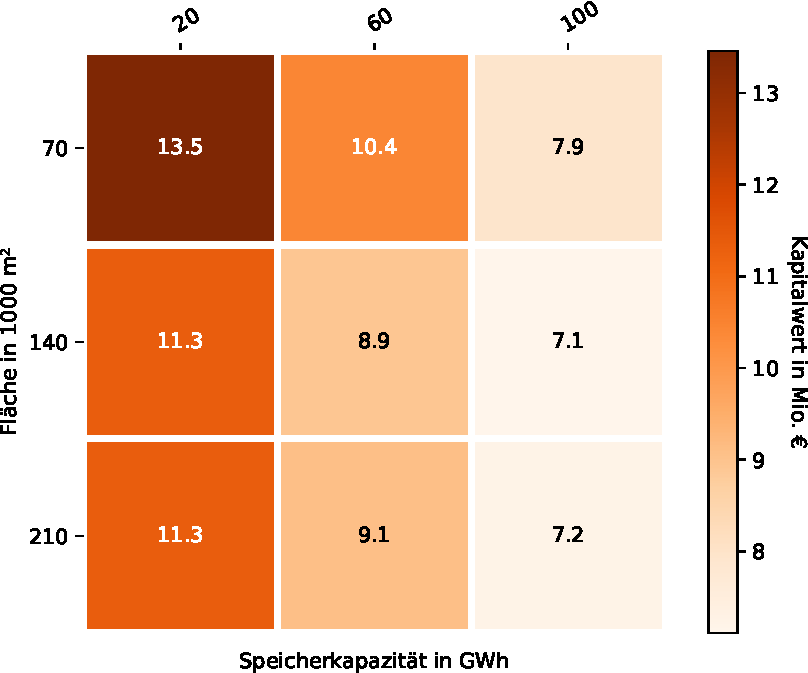
\includegraphics[width=0.8\textwidth]{PV_Heatmap_relNPV-cropped.pdf}
		\captionof{figure}[Darstellung aller Kapitalwerte innerhalb des Photovoltaik-Szenarios]{Darstellung einer Heatmap aller Kapitalwerte innerhalb des Photovoltaik-Szenarios. Dunkel dargestellte Fläche zeigen gegenüber helleren Flächen einen erhöhten Kapitalwert an.}
		\label{figure: Heatmap Photovoltaik}
	\end{figure}

Der höchste Kapitalwert mit 19,5~Mio.~\euro\ wird bei dem ST1-Konzept erreicht. Mit zunehmender Kollektorfläche auf 140.000~m² nimmt der Kapitalwert zunächst um 9,8~Mio.~\euro\ ab - bei einer Vergrößerung auf 210.000~m² um weitere 9,5~Mio.~\euro. Das zeigt, dass bei den gegebenen Umweltbedingungen eine zunehmende Kollektorfläche in dem betrachteten Bereich zu einer überproportionalen Abnahme des Kapitalwerts führt. Hieraus folgt, dass das Verhältnis aus gewonnenem Nutzen durch eine zunehmende Kollektorfläche und den zusätzlichen Kosten abnimmt. Außerdem kann an dieser Stelle zunächst davon ausgegangen werden, dass die optimale Kollektorfläche erst bei deutlich geringeren Werten erreicht wird. Bei einer Speicherkapazität von 60~GWh ist die Abnahme des Kapitalwerts ungefähr gleich der Abnahme bei 20~GWh. Erst bei der höchsten Kapazität von 100~GWh ist zu erkennen, dass die Abnahme des Kapitalwerts geringer wird. Bei einer Zunahme der Fläche auf 140.000~m² verringert sich der Kapitalwert an dieser Stelle nur um 7,5~Mio.~\euro. Daraus kann gefolgert werden, dass bei dieser Speicherkapazität die optimale Kollektorfläche größer ist und der Auslegungspunkt bei 70.000~m² somit dichter an einem lokalen Maximum liegt. Dies ist insofern plausibel, da davon ausgegangen werden kann, dass eine zunehmende Kollektorfläche einen größeren saisonalen Wärmespeicher erfordert. Analog dazu kann Abbildung \ref{fig: Heatmaps Solarthermie a}, aufgrund der relativ konstanten Abnahme des Kapitalwerts bei einer Steigerung der Kapazität von 60 auf 100~GWh, entnommen werden, dass die optimale Speichergröße unterhalb von 20~GWh liegt.

Abbildung \ref{fig: Heatmaps Solarthermie b} stellt die Kapitalwerte des ST2-Konzeptes dar. Wie bei dem ST1-Konzept ist der Kapitalwert bei einer Fläche von 70.000~m² und einer Speicherkapazität von 20~GWh am höchsten, liegt jedoch mit 13,5~Mio.~\euro\ etwas unter dem Ergebnis des ST1-Konzepts. Eine Zunahme der Kollektorfläche hat hier die selben Auswirkungen wie in ST1. Die Kapitalwerte fallen konstant um einen Wert von ca. 10~Mio.~\euro. Ebenso ist zu erkennen, dass die Abnahme bei einer Speicherkapazität von 60~GWh und 100~GWh zunächst geringfügig voneinander abweicht, bei einer Fläche von 140.000~m² und 210.000~m² jedoch gleich groß ist und zu identischen Kapitalwerten führt. In diesem Bereich scheinen sich der Nutzen und die zusätzlichen Kosten aufzuheben. Im Gegensatz zum ST1-Konzept ändert sich der Kapitalwert bei einer Zunahme der Speicherkapazität von 20 auf 60~GWh -~und konstant bleibender Fläche von 70.000~m²~- zunächst nur minimal, was darauf hindeutet, dass zwischen diesen Werten ein lokales Maximum zu finden ist.

Gegenüber den Solarthermie-Konzepten zeigen die \ac{PV}-Szenarien (Abbildung \ref{figure: Heatmap Photovoltaik}) ein etwas anderes Verhalten. Der höchste Kapitalwert liegt hier zwar ebenfalls bei der geringsten Fläche und Speicherkapazität, es wird jedoch bei zunehmender Kollektorfläche und Kapazität kein Kapitalwert negativ. Das heißt, dass alle Szenarien dem Referenzsystem aus ökonomischer Sicht vorzuziehen sind. Eine Zunahme der Modulfläche führt zunächst bei allen Speicherkapazitäten zu einer Abnahme des Kapitalwerts. Eine weitere Erhöhung der Fläche hat jedoch keinen weiteren Einfluss auf den Kapitalwert. Die gleichbleibenden Kapitalwerte bei 140.000 und 210.000~m² sprechen dafür, dass mit zunehmender Modulfläche ein anwachsender Anteil des \ac{PV}-Stroms am Spotmarkt vermarktet wird. Dies liegt daran, dass das \ac{PV}-System mit zunehmender Fläche entsprechend mehr am Spotmarkt agiert und somit eine zusätzliche Einnahmequelle vorliegt, die den zunehmenden Kosten zunächst entgegen wirkt. Der Punkt, an dem die zusätzlichen Investitions- und Betriebskosten den Nutzen durch größere Anlagendimensionierungen übersteigen, wird bei diesem Konzept deutlich später erreicht. 

	\begin{figure}[ht]
		\centering
		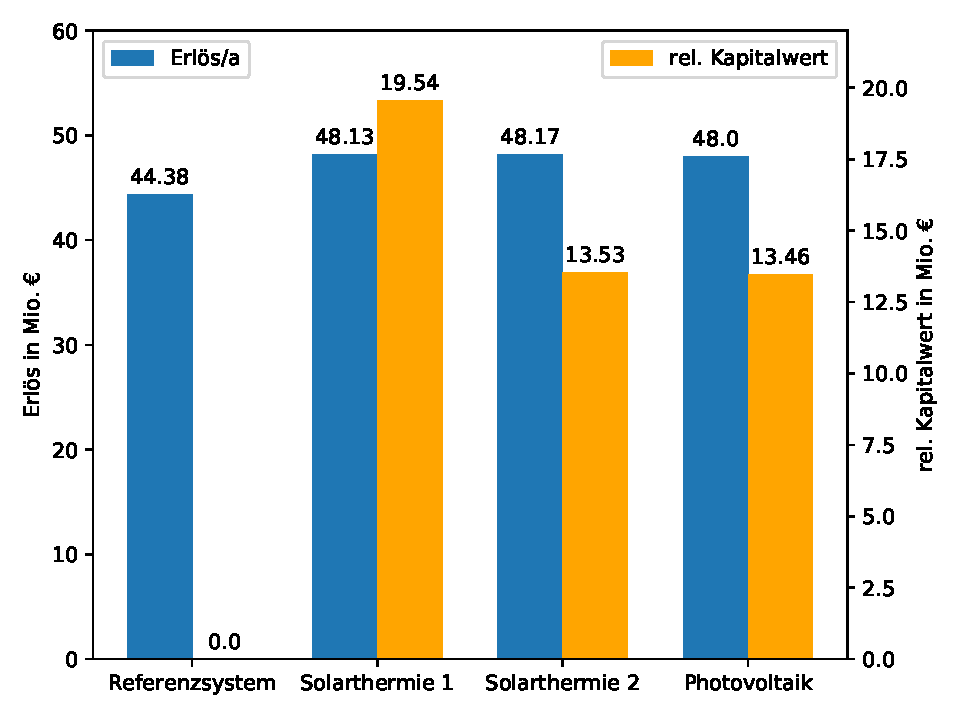
\includegraphics[width=0.8\textwidth]{Verbesserung/Erloes_K0_bester_Szenarien-cropped.pdf}
		\captionof{figure}[Gegenüberstellung der Erlöse und Kapitalwerte der wirtschaftlichsten Szenarien]{Darstellung der Erlöse und Kapitalwerte der verschiedenen Konzepte bei einer Kollektorfläche von 70.000~m² und einer Speicherkapazität von 20~GWh. Die Kapitalwerte der Alternativkonzepte werden auf das Referenzsystem bezogen, weshalb dieses mit einem Kapitalwert 0 angezeigt wird.}
		\label{figure: Erloes_K0_bester_Szenarien}
	\end{figure}

Abbildung \ref{figure: Erloes_K0_bester_Szenarien} stellt die, für eine genauere Untersuchung des Anlagenverhaltens ausgewählten Szenarien aller Konzepte vergleichend gegenüber. Es handelt sich hierbei stets um die Szenarien bei einer Kollektorfläche von 70.000~m² und einer Speicherkapazität von 20~GWh, da sich diese Auslegung als die wirtschaftlich attraktivste für alle Konzepte - unter den betrachteten Dimensionierungen - erwiesen hat. Es ist zu erkennen, dass im Betrachtungszeitraum alle Alternativkonzepte einen deutlich höheren Erlös gegenüber dem Referenzsystem erwirtschaftet haben. Trotzdem zeigt sich, dass der Kapitalwert des ST1-Konzepts erheblich größer ausfällt als beim ST2-, oder PV-Konzept. Dies ist über die zusätzlichen Investitionskosten der installierten Wärmepumpen zu erklären, die im PV-Konzept 12,5~Mio.~\euro\ und im ST2-Konzept 6,25~Mio.~\euro\ betragen. Darüber hinaus ist zu erkennen, dass die, durch eine zusätzlich installierte \ac{WP} und \ac{STTES} erhöhten Erlöse des Solarthermie~2 Konzepts, die Investitionskosten der Anlagen nicht kompensieren können.

Die folgenden Abschnitte werden das Anlagenverhalten innerhalb der ausgewählten Szenarien genauer betrachten. Außerdem wird für jedes Konzept eine Einflussanalyse durchgeführt, um zu identifizieren, welche Technologie welchen Einfluss auf das entsprechende Betriebsergebnis hat.

\subsubsection{Ergebnisse der Einsatzoptimierung Solarthermie 1}
Abbildung \ref{figure: Jahresdauerlinie_Solarthermie1} können die Jahresdauerlinien des Solarthermie 1 Konzeptes entnommen werden. Es zeigt sich, dass der Elektrodenheizkessel als Wärmeversorgungstechnologie fast komplett verdrängt worden ist - er wird über den betrachteten Zeitraum bloß 246~h betrieben. Die Betriebsstunden des \acl{SLK} bleiben hingegen fast identisch zum Referenzsystem - er wird mit 1870~h nur etwas weniger betrieben. Es ist jedoch zu erkennen, dass der \ac{SLK} deutlich länger im Nennbetriebspunkt betrieben wird. Ebenso hat sich der Betrieb des \ac{GuD} insofern verändert, dass die Betriebsstunden mit ca. 5.031~h im Vergleich zum Referenzsystem deutlich geringer ausfallen, die Anlage  jedoch erheblich länger unter Volllast betrieben wird. An dieser Stelle wird ausschließlich die Wärmebereitstellung des \ac{GuD} betrachtet.
	\begin{figure}[ht]
		\centering
		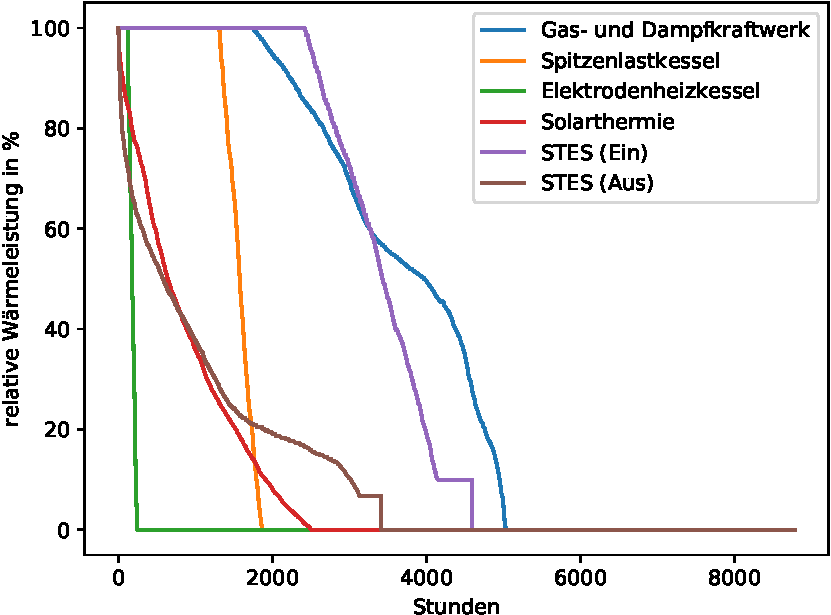
\includegraphics[width=0.8\textwidth]{Verbesserung/Jahresdauerlinie_Solarthermie1-cropped.pdf}
		\captionof{figure}[Jahresdauerlinien des Solarthermie 1-Konzepts]{Darstellung der Jahresdauerlinie aller verwendeten Technologien innerhalb des Solarthermie 1 Konzepts bei einer Kollektorfläche von 70.000~m² und einer Kapazität von 20~GWh}
		\label{figure: Jahresdauerlinie_Solarthermie1}
	\end{figure}
Die Jahresdauerlinie der Solarthermie-Anlage zeigt, dass nur wenige Stunden im Jahr eine volle Sonneneinstrahlung vorliegt. Erst ab einer Leistung von 60\% nehmen die Betriebsstunden der Anlage merklich zu. Insgesamt stellt die Solaranlage über das betrachtete Jahr 2.503~h Wärme bereit. 

Vergleicht man die Technologien hinsichtlich der insgesamt produzierten Wärme, liefert die \ac{GuD}-Anlage 84,77\% der Wärmeproduktion. Dies ist nur geringfügig unterhalb der anteiligen Produktion innerhalb des Referenzsystems. Ähnlich verhält es sich beim Betrieb des Spitzenlastkessels, der mit 7,32\% knapp 2,5 Prozentpunkte unterhalb des entsprechenden Werts im Referenzsystem liegt. Beim \ac{EHK} konnte bereits über die Betriebsstunden abgelesen werden, dass diese Technologie kaum einen Beitrag an der Wärmeproduktion leistet - nur 0,83\%. Die Solarthermie-Anlage schafft in diesem Konzept einen Anteil von 7,08\% an der gesamten Wärmeproduktion. Die Wärmegestehungskosten dieses Systems betragen 30,08~\euro/MWh und liegen damit 2,7~\euro/MWh unterhalb des Referenzsystem-Werts.

Bei dem Betrieb des \ac{STES} kann den Jahresdauerlinien entnommen werden, das er knapp 2500~h des Jahres mit dem maximal möglichen Wärmestrom geladen wird. Dem gegenüber ist der Speicher in dem betrachteten Jahr nie unter Volllast entladen worden. Die Fläche unterhalb der Kurven fürs Auf- und Entladen weichen deutlich voneinander ab, was an den unterschiedlich modellierten maximal möglichen Wärmeströmen liegt. Wie in Kapitel \ref{subsection: Solarthermie 1} beschrieben wurde, ist der Speicher so modelliert worden, dass er höchstens mit dem maximal möglichen Wärmestrom der Solaranlage geladen werden kann. Beim Entladen war der höchst mögliche Wärmestrom hingegen mit der maximalen Heizlast innerhalb des Jahres modelliert worden. Die Darstellung in Dauerlinien zeigt also, dass es besser gewesen wäre, die maximal mögliche Aufladung größer und die Entladung entsprechend geringer zu wählen.
	\begin{figure}
		\centering
		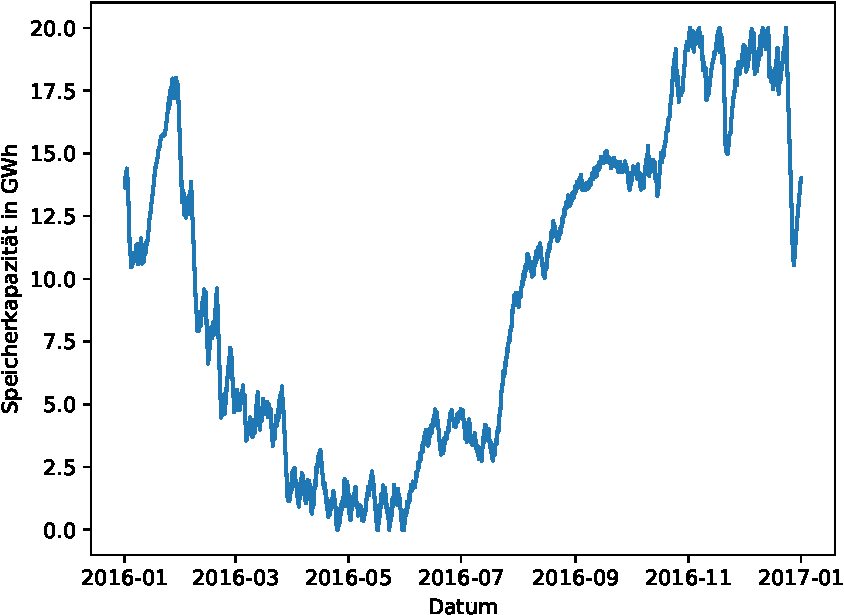
\includegraphics[width=0.8\textwidth]{Verbesserung/Speicherverhalten_Solarthermie1-cropped.pdf}
		\captionof{figure}[Ladezustand des saisonalen Wärmespeichers innerhalb des Solarthermie 1-Konzepts]{Illustration des Ladezustands des saisonalen Wärmespeichers innerhalb des Solarthermie 1-Konzepts über den betrachteten Zeitraum}
		\label{figure: Speicherkapazität_Solarthermie1}
	\end{figure}

Abbildung \ref{figure: Speicherkapazität_Solarthermie1} zeigt zu jedem Zeitpunkt des betrachteten Jahres den Ladezustand des Wärmespeichers. Nachdem zunächst ca. 2~GWh aus dem Speicher entnommen werden, wird er im Februar bis auf ca. 17,5~GWh geladen. Daran anschließend wird der Speicher bis in den Mai überwiegend entladen. Von Anfang Juni bis Ende Juli bildet sich eine kleine Erhöhung aus, in der der Speicher wieder auf knapp 5~GWh geladen wird. Von August bis November wird der Speicher primär aufgeladen. Im Winter wird er mehrmals entladen - wird aber in kurzer Zeit wieder auf die maximale Kapazität aufgeladen. Dieses Verhalten ist durch tendenziell erhöhte Strompreise und den damit einhergehenden Betrieb der \ac{GuD}-Anlage zu erklären. Welchen Einfluss die Solarthermie auf den Verlauf der Speicherkapazität hat wird in der an diesen Abschnitt angrenzenden Einflussanalyse untersucht.
	\begin{figure}
		\centering
		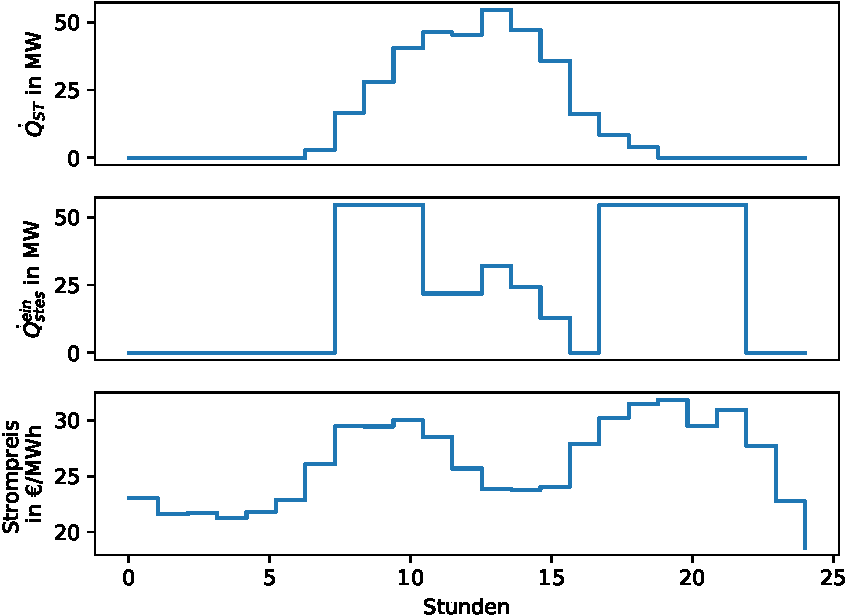
\includegraphics[width=0.8\textwidth]{Verbesserung/Solarthermie_1_Verhalten-cropped.pdf}
		\captionof{figure}[Darstellung der solaren Wärme über Speicherbeladung und Strompreis für das ST1-Konzept]{Darstellung der solaren Wärme $\dot{Q}_{ST}$ über dem Speicher zugeführten Wärmestrom $\dot{Q}_{stes}^{ein}$ sowie den Strompreisen für den 11.06.2016 - den Tag mit der höchsten Sonneneinstrahlung im Betrachtungszeitraum}
		\label{figure: Verhalten_Solarthermie1}
	\end{figure}
	
Zunächst soll jedoch veranschaulicht werden nach welchen Prinzipien der Speicher beladen wird. Zu diesem Zweck wird in Abbildung \ref{figure: Verhalten_Solarthermie1} der Solarthermie-Ertrag über dem Wärmestrom in den \ac{STES} und jeweiligen Strompreisen am Spotmarkt dargestellt. Es ist sofort zu erkennen, dass der Speicher - trotz des erheblichen Wärmestroms aus der Solarthermie - primär durch die \ac{GuD}-Anlage aufgeladen wird. Dies kann daraus abgeleitet werden, dass die Aufladung des Speichers mit dem Strompreis korreliert. Ein erhöhter Strompreis am Spotmarkt führt dazu, dass das \ac{GuD} verstärkt betrieben wird. Gleichzeitig kann Abbildung \ref{figure: Verhalten_Solarthermie1} entnommen werden, dass zumindest ein Teil der durch die Solarthermie bereitgestellten Wärme genutzt wird, um den Speicher zu laden. Dies ist zwischen Stunde 11 und Stunde 16 der Fall.

\subsubsection*{Einflussanalyse des ST1-Konzepts}
Abbildung \ref{figure: Erloes_K0_bester_Szenarien} hat bereits gezeigt, dass das Solarthermie 1 Konzept - die Einbringung einer Solarthermie-Anlage und eines saisonalen Wärmespeichers - einen ökonomischen Vorteil gegenüber dem Referenzsystem darstellt. An dieser Stelle wird kurz untersucht, welchen Beitrag die einzelnen Technologien zu diesem Ergebnis geleistet haben.

Um den Einfluss der Solarthermie und des \ac{STES} zu untersuchen sind diese Technologien einzeln dem Referenzsystem hinzugefügt worden. Zunächst soll der Einfluss des \ac{STES} untersucht werden. Zu diesem Zweck ist der Solarthermie-Ertrag innerhalb des ST1-Konzepts auf 0 gesetzt worden. Es zeigt sich nach Abbildung \ref{fig: Jahresdauerlinie_Einfluss_ST1}, dass das Referenzsystem einzig durch den Einsatz eines Wärmespeichers deutlich effizienter betrieben werden kann. Der Speicher sorgt für eine Entkopplung der Wärmeproduktion sowie des Bedarfs und führt somit dazu, dass das \ac{GuD} verstärkt bei Nennlast Wärme bereitstellt. 

Ein Vergleich der Jahresdauerlinien ohne Solarthermie zeigt darüber hinaus, dass sich das Betriebsverhalten der Anlagen kaum von dem System mit Solarthermie unterscheidet. Der \ac{EHK} ist genauso aus der Wärmeproduktion verdrängt worden, was zeigt, dass die Verdrängung einzig an der Verwendung eines Wärmespeichers liegt. Demgegenüber zeigt die übers Jahr aufgetragene relative Speicherkapazität in Abbildung \ref{fig: Speicherkapazität_Einfluss_ST1}, in der die Differenz zwischen dem Ladezustand des Systems mit und ohne Solarthermie abgebildet wird, einen deutlichen Unterschied des Ladeverhaltens. Es ist zu erkennen, dass der Ladezustand des Speichers zwischen August und Ende Oktober ohne Wärme aus der Solarthermie um bis zu 6~GWh niedriger ist. Dies zeigt, dass Solarthermie durchaus saisonal gespeichert wird und stützt somit das in Abbildung \ref{figure: Verhalten_Solarthermie1} dargestellte Verhalten, dass die Wärme aus der Solarthermie anteilig zur Ladung des Speichers genutzt wird. Ein kleinerer Ausschlag ist im März erkennbar. Zu dieser Zeit werden die ersten nennenswerten Erträge über die Solarthermie bereitgestellt. Zwischen diesen Zeiträumen unterscheidet sich der Ladezustand um maximal 1~GWh, was dafür spricht, dass die Solarthermie zu dieser Zeit mit einer niedrigen Wärmelast bevorzugt direkt zur Wärmebereitstellung genutzt wird.
	\begin{figure}
		\begin{subfigure}[b]{0.48\textwidth}
			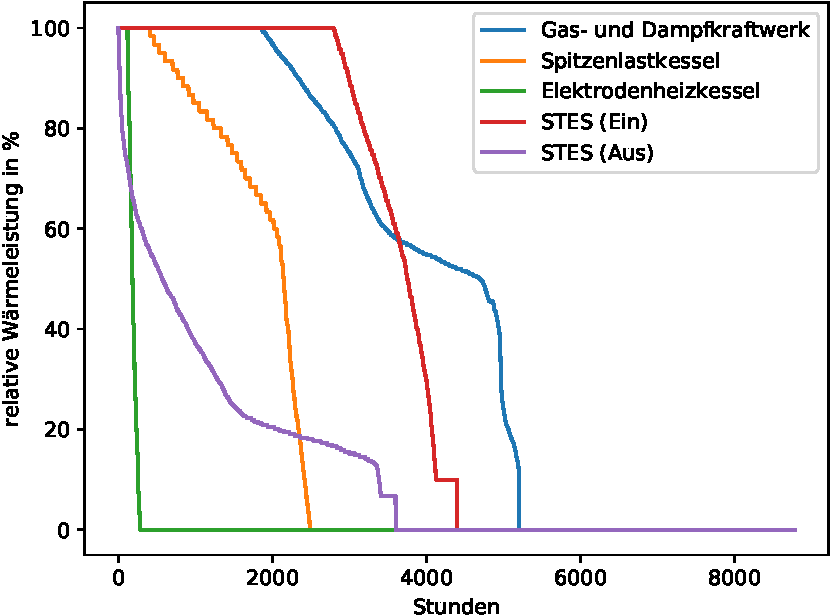
\includegraphics[width=1\textwidth]{Verbesserung/ST1_Jahresdauerlinie_Einfluss_STES-cropped.pdf}
			\subcaption{Jahresdauerlinien}
			\label{fig: Jahresdauerlinie_Einfluss_ST1}
		\end{subfigure}
		\hfill
		\begin{subfigure}[b]{0.48\textwidth}
			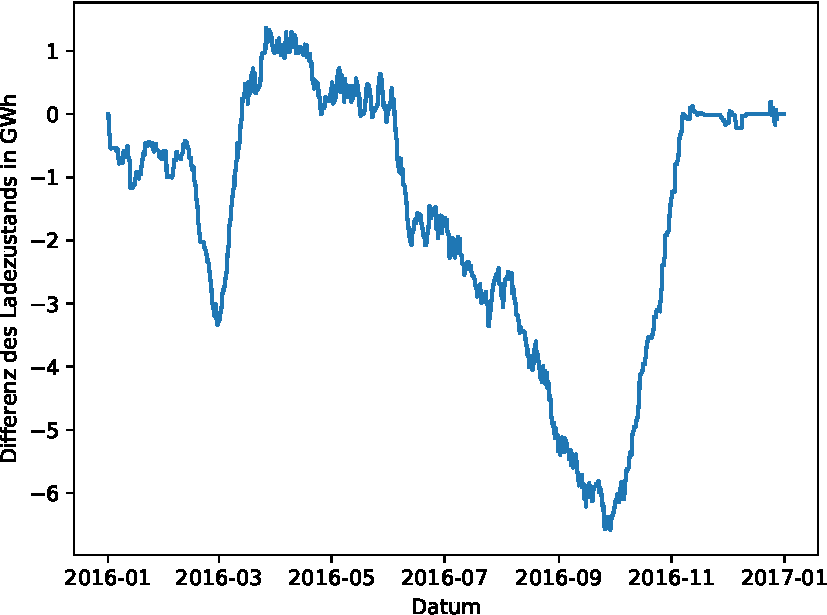
\includegraphics[width=1\textwidth]{Verbesserung/ST1_relSpeicherkap_Einfluss_STES-cropped.pdf}
			\subcaption{relative Speicherkapazität}
			\label{fig: Speicherkapazität_Einfluss_ST1}
		\end{subfigure}
		\caption[Verhalten der Anlagen des ST1-Konzepts ohne den Ertrag aus der Solarthermie-Anlage]{Verhalten der Anlagen des ST1-Konzepts ohne den Ertrag aus der Solarthermie-Anlage. In (a) werden die Jahresdauerlinien dargestellt, während in (b) die Differenz beim Ladezustand zwischen dem ST1-Konzept mit und ohne Solarthermie dargestellt wird. Ein negative Ausschlag bedeutet, dass der Ladezustand des Speichers mit Solarthermie zu diesem Zeitpunkt höher ist.}
		\label{fig: Einfluss}
	\end{figure}


Aus rein ökonomischer Sicht zeigt sich, dass das Hinzufügen eines Wärmespeichers - zur Entkopplung der Wärmeproduktion und des Bedarfs - attraktiver ist, als die Kombination aus Solarthermie und Speicher. Der Kapitalwert des Referenzsystems steigt allein durch den Wärmespeicher mit einer Kapazität von 20~GWh um 33,16~Mio.~\euro, was ungefähr 170\% der Kombination aus Solarthermie und Speicher entspricht. Gleichzeitig sinkt der Kapitalwert des Referenzsystems um 17,71~Mio.~\euro, wenn ausschließlich eine Solaranlage mit 70.000~m² hinzugefügt wird. Der fehlende Speicher sorgt dafür, dass es nicht möglich ist 100\% des Solar-Ertrags zu verwenden. Tatsächlich werden ohne einen Speicher nur ca. 1/4 der solarthermischen Wärme genutzt. Dies sorgt für den niedrigen Kapitalwert. 

Die Einflussanalyse des Solarthermie 1-Konzepts hat gezeigt, dass bei den zugrunde gelegten regulatorischen Rahmenbedingungen und Brennstoffkosten aus rein ökonomischer Sicht die einfache Ergänzung des Referenzsystems um einen Wärmespeicher die attraktivste Maßnahme darstellt. Dies wird in Tabelle \ref{tabelle: Übersicht Einflussanalyse ST1} veranschaulicht. Es ist klar zu erkennen, dass das Ergebnis des ST1-Konzepts hauptsächlich aufgrund des verwendeten Speichers gut ausfällt. Die Verwendung der Solarthermie erhöht den Erlös nur um 400.000~\euro, senkt den Kapitalwert durch die hohen Investitionskosten jedoch erheblich. 
	\begin{center}
		\captionof{table}{Übersicht über die Ergebnisse der Einflussanalyse des Solarthermie 1-Konzepts} 
		\label{tabelle: Übersicht Einflussanalyse ST1}
		\begin{tabular}{lcccc}
			\hline 
			 &  & Erlös M\euro/a & Kapitalwert M\euro & \ac{LCOH} \euro/MWh\tabularnewline
			 
			\hline 
			Solarthermie 1 (normal)  &  & 48,13 & 19,5 & 30,08 \tabularnewline
			nur mit \ac{STES}		 &  & 47,68 & 33,16 & 28,26 \tabularnewline
			nur mit Solarthermie 	 &  & 44,48 & -17,71 & 35,08 \tabularnewline		
			\hline
		\end{tabular}
	\end{center}

\subsubsection{Ergebnisse der Einsatzoptimierung Solarthermie 2}
Das Solarthermie 2-Konzept stellt mit einer zusätzlichen Wärmepumpe und einem Kurzzeitspeicher (\acs{STTES}) ein Konzept dar, bei dem die Solarthermie mit anderen Technologien zur Wärmebereitstellung kombiniert wird. Die \ac{WP} sollte den Anteil an \ac{P2H} in dem Wärmeversorgungssystem erhöhen und somit ein Wärmesystem mit erhöhtem \ac{P2H}-Anteil abbilden. Wie bereits im vorangegangen Abschnitt zum ST1-Konzept, soll an dieser Stelle das Betriebsverhalten der Anlagen - als Ergebnis der Einsatzoptimierung - genauer betrachtet werden. Daran anschließend wird eine Einflussanalyse durchgeführt, die den Einfluss der neu hinzugekommenen Technologien auf das Betriebsergebnis untersuchen wird. 

Die Jahresdauerlinien des Solarthermie 2-Konzepts werden in \ref{figure: Jahresdauerlinie_Solarthermie2} dargestellt. Aufgrund der Tatsache, dass die Solarthermie als fixe Eingangsgröße in das Optimierungsmodell abgebildet worden ist, unterscheidet sich der Betrieb der Solaranlage nicht von dem aus ST1. Wie beim ST1-Konzept ist der \ac{EHK} als Wärmeversorgungstechnologie hier ebenfalls fast komplett verdrängt worden - interessanterweise bleibt der Anteil an der Wärmeproduktion, trotz der zusätzlichen \acl{WP}, nahezu unverändert. Gleiches gilt für den Betrieb des \ac{SLK}, der in diesem Konzept nur 35~h weniger als beim ST1-Konzept betrieben wird. Ein entgegengesetzter Effekt ist beim Betrieb des \ac{GuD} zu beobachten, welches mit 4.684 Betriebsstunden zwar knapp 350~h weniger im Betrachtungszeitraum betrieben wurde - jedoch 700~h länger unter Volllast Wärme bereitgestellt hat. Dies ist vor allem durch die Verwendung des Kurzzeitspeichers zu erklären, der im Gegensatz zum modellierten \ac{STES} auf stündlicher Basis ge- und entladen werden kann. Zur Wärmepumpe ist zu sagen, dass sie überwiegend zwischen 60\% und 70\% gearbeitet hat. Dies liegt unter anderem daran, dass die Leistungszahl von den Umweltbedingungen und der Vorlauftemperatur des Netzes abhängt, und diese über weite Teile des Jahres keinen optimalen Betrieb erlauben.
	\begin{figure}[ht]
		\centering
		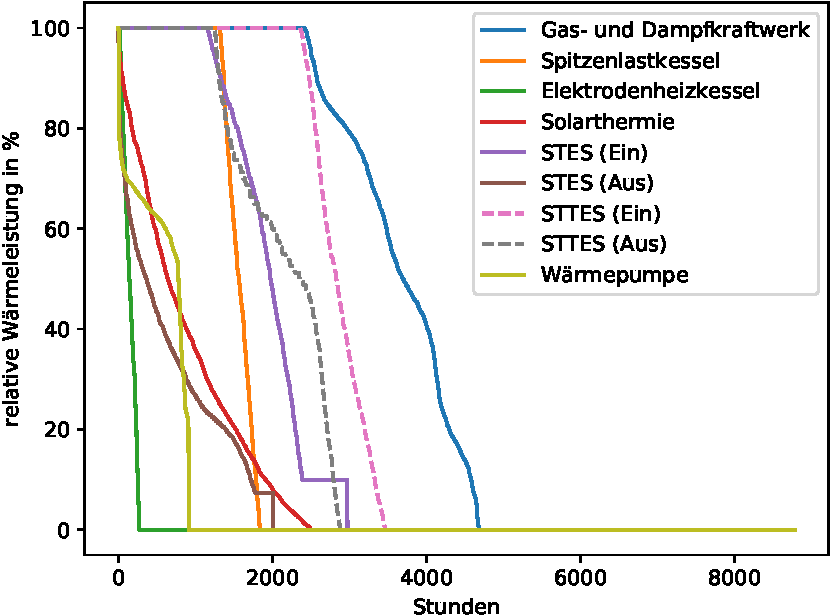
\includegraphics[width=0.8\textwidth]{Verbesserung/Jahresdauerlinie_Solarthermie2-cropped.pdf}
		\captionof{figure}[Jahresdauerlinie Solarthermie 2]{Abbildung der Jahresdauerlinien des Solarthermie 2-Konzepts. Dargestellt wird die relative Wärmeleistung der verwendeten Technologien über den Betriebsstunden bei einer Kollektorfläche von 70.000~m² und einer Speicherkapazität von 20~GWh}
		\label{figure: Jahresdauerlinie_Solarthermie2}
	\end{figure}

Anhand der Jahresdauerlinie ist zu erkennen, dass der \ac{STES} deutlich weniger genutzt wird als im ST1-Szenario. Der Verlauf der Be- und Entladung hat sich jedoch prinzipiell nicht verändert. Zum Großteil wird der Speicher noch immer unter Volllast aufgeladen, während das Entladen hauptsächlich in Teillast erfolgt. Die Gründe sind dieselben wie bereits beim ST1-Konzept. Der Kurzzeitspeicher wird zum größten Teil unter Volllast aufgeladen. Die Entladung findet zu ungefähr der Hälfte unter Volllast statt. Der Unterschied zwischen beiden Kurven liegt beim Kurzzeitspeicher einzig an dem Wirkungsgrad von 75\%. 

Das Speicherverhalten hat sich im Vergleich zum ST1-Konzept nur geringfügig verändert. Dominiert wird das Verhalten immer noch von den Strompreisen - hohe Strompreise führen zu einem wirtschaftlichen Betrieb der \ac{GuD}-Anlage, welche dann zum Laden des Speichers genutzt wird. Um das Anlagenverhalten zu veranschaulichen ist in Abbildung \ref{figure: Verhalten_Solarthermie2} die solarthermisch gewonnene Wärme für den 09. und 10.05.2016 über der Speicherbeladung $\dot{Q}^{ein}$, dem Wärmestrom der Wärmepumpe $\dot{Q}_{WP}$ und den Strompreisen aufgetragen. Es ist zu erkennen, dass der saisonale Speicher und der Kurzzeitspeicher ähnlich geladen werden. Ein erhöhter Strompreis am Morgen und Abend führt bei beiden Speichern zu einer Beladung mit dem maximal möglichen Wärmestrom. Die Wärmepumpe wird in dem Beispiel nachts bei fehlender Solarthermie genutzt, um Wärme bereitzustellen - diese wird ausschließlich ins Netz eingespeist. Die solarthermische Wärme wird wie in ST1 anteilig zur Speicherung genutzt. An den dargestellten Tagen wird jedoch vorzugsweise der Kurzzeitspeicher genutzt. 
	\begin{figure}
		\centering
		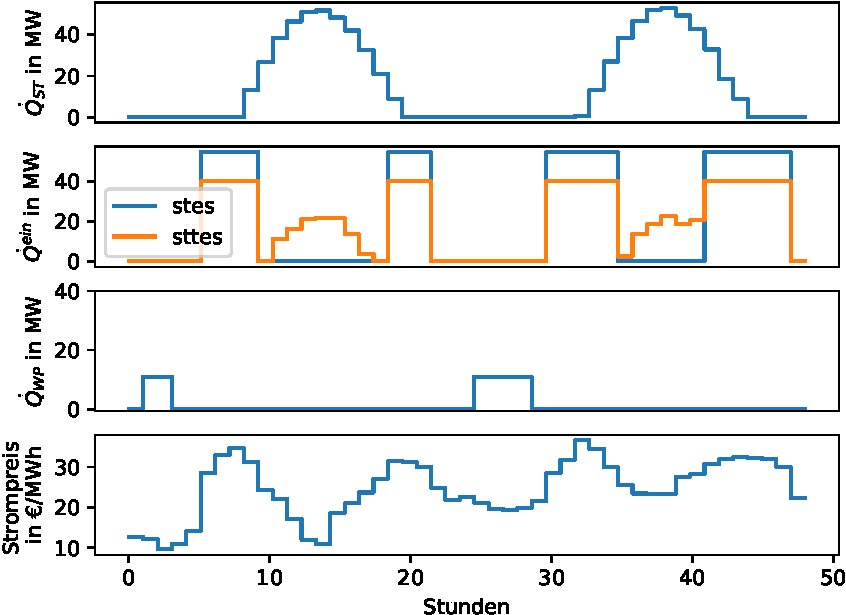
\includegraphics[width=0.8\textwidth]{Verbesserung/Solarthermie_2_Verhalten_09_05-cropped.pdf}
		\captionof{figure}[Illustration der solaren Wärme über Speicherbeladung und Strompreis für das ST2-Konzept]{Illustration des Solarthermie-Ertrags $\dot{Q}_\text{ST}$, der Speicherbeladung $\dot{Q}^{ein}$ des \ac{STES} und \ac{STTES} über der Wärmeabgabe durch die Wärmepumpe $\dot{Q}_{WP}$ und den Strompreisen für den 09/10.05.2016}
		\label{figure: Verhalten_Solarthermie2}
	\end{figure}

Insgesamt hat sich die Wärmeproduktion innerhalb des ST2-Szenarios kaum verändert. Der Anteil des \ac{GuD} ist weiter auf 82,39\% gesunken - stellt jedoch weiterhin die dominierende Technologie dar. Die Wärmeproduktion des \ac{SLK} hat sich auf 7,20\%  und die des \ac{EHK} auf 0,69\% reduziert. Die Wärmeproduktion der \ac{WP} beträgt anteilig an der gesamten Produktion 2,75\% und ist für die reduzierten Anteile der anderen Technologien verantwortlich. Der Solarthermie-Anteil bleibt im Wesentlichen unverändert.

\subsubsection*{Einflussanalyse des ST2-Konzepts}
Bereits für das ST1-Szenario ist der Einfluss der Solarthermie und des \ac{STES} auf das Ergebnis der Optimierung untersucht worden. Dieser Abschnitt befasst sich daher ausschließlich mit der Wärmepumpe sowie dem Kurzzeitspeicher und deren Auswirkungen auf das ST2-Konzept.

Zunächst wird der Einfluss der Wärmepumpe untersucht indem diese aus der Optimierung entfernt wird. Es zeigt sich, dass durch die zusätzliche \ac{WP} das Betriebsergebnis des ST1-Konzept quasi nicht verbessert wird. Der Erlös mit einer zusätzlich installierten Wärmepumpe hat sich um 0,04~Mio.~\euro\ erhöht. Eine Umverteilung der Wärmeproduktion durch den Einsatz der Wärmepumpe hat also nur einen geringen Einfluss auf das Betriebsergebnis der Optimierung. Durch die zusätzlichen Investitionskosten hat sich der Kapitalwert des Konzepts jedoch auf 13,5~Mio.~\euro\ reduziert. 

Ein anderer Effekt ist zu beobachten, wenn ausschließlich der Kurzzeitspeicher als Ergänzung zum ST1-Konzept betrachtet wird. In diesem Fall erhöht sich der Kapitalwert auf 18,63~Mio.~\euro\ und liegt damit nur knapp unterhalb dem Kapitalwert des ST1-Konzepts. Offenbar hat der zusätzliche Speicher einen positiven Einfluss auf das Betriebsergebnis. Liegt diese Verbesserung jedoch an dem zusätzlichen Speicher, der stündlich ge- und entladen werden kann und somit einen parallelen Betrieb zum \ac{STES} ermöglicht, oder ruht die Verbesserung in der Tatsache, dass insgesamt ein höherer Wärmestrom gespeichert werden kann. Um diese Frage zu beantworten ist der maximal mögliche Wärmestrom zur Beladung des \ac{STES} verdoppelt (dies entspricht ungefähr der Summe des \ac{STES} und \ac{STTES}) und eine Betriebsoptimierung ohne einen Kurzzeitspeicher durchgeführt worden. Es zeigt sich, dass allein durch einen größeren Wärmestrom, mit dem der \ac{STES} beladen wird, ein deutlich besseres Betriebsergebnis erreicht wird. Darüber hinaus führt dies zu einer, mit 2631~h unter Volllast, effizienteren Nutzung des \ac{GuD}. Der Kapitalwert steigt auf 21,95~Mio.~\euro\ und liegt -~aufgrund der fehlenden Investitionskosten für den zusätzlichen Speicher~- oberhalb des Kapitalwerts des \ac{STTES}-Systems. Dieses Ergebnis zeigt, welchen Einfluss die Beladung des Speichers auf die Optimierung hat und dass der angenommene, maximale Wärmestrom im Prinzip zu niedrig angesetzt worden ist.

Abgesehen von dem Betriebsergebnis hat der zusätzliche Wärmespeicher jedoch einen erheblichen Einfluss auf die Art und Weise, wie der \ac{STES} betrieben wird. Abbildung \ref{fig: Einfluss_Speicher_Solar_2} stellt den Ladezustand des saisonalen Speichers gegenüber. Die Grafik \ref{fig: Speicherkapazität_ST2} illustriert hier das Speicherverhalten des \ac{STES} bei Verwendung eines Kurzzeitspeichers. Demgegenüber stellt Grafik \ref{fig: Speicherkapazität_Einfluss_ST2} den Ladezustand ohne die Verwendung eines Kurzzeitspeichers dar. Es ist zu erkennen, dass ein zusätzlicher Speicher den Betrieb des \ac{STES} glättet. Die Verwendung eines zusätzlichen Speichers hat also einen erheblichen Einfluss auf die Betriebsweise des \ac{STES}.
	\begin{figure}[ht]
		\begin{subfigure}[b]{0.48\textwidth}
			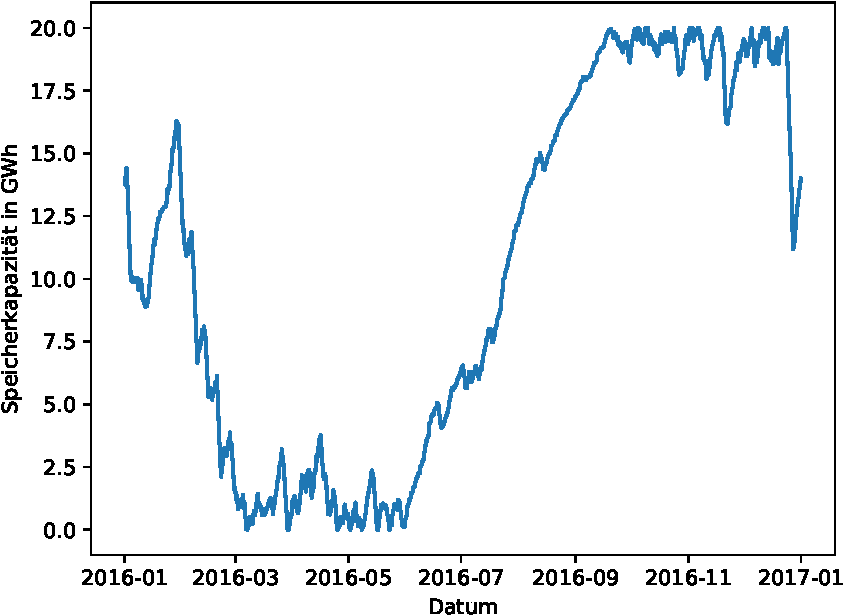
\includegraphics[width=1\textwidth]{Verbesserung/Speicherverhalten_Solarthermie2-cropped.pdf}
			\subcaption{mit \ac{STTES}}
			\label{fig: Speicherkapazität_ST2}
		\end{subfigure}
		\hfill
		\begin{subfigure}[b]{0.48\textwidth}
			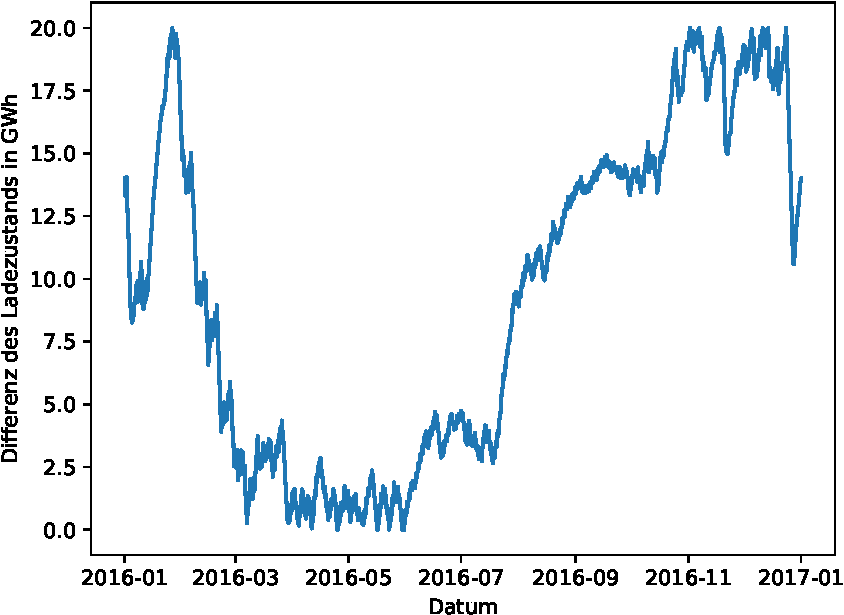
\includegraphics[width=1\textwidth]{Verbesserung/Speicherverhalten_Solarthermie2_woSTTES-cropped.pdf}
			\subcaption{ohne \ac{STTES}}
			\label{fig: Speicherkapazität_Einfluss_ST2}
		\end{subfigure}
		\caption[Vergleich des saisonalen Speicherverhaltens mit und ohne Kurzzeitspeicher]{Gegenüberstellung des saisonalen Speicherverhaltens mit und ohne Kurzzeitspeicher. In Teil (a) wird der Ladezustand des Speichers mit Kurzzeitspeicher - in Teil (b) ohne dargestellt.}
		\label{fig: Einfluss_Speicher_Solar_2}
	\end{figure}

Tabelle \ref{tabelle: Übersicht Einflussanalyse ST2} fasst die ökonomischen Ergebnisse der Einflussanalyse kurz zusammen. Die Tatsache, dass der Erlös der Optimierung nur mit \acl{STTES} höher ist, als der Erlös des normalen ST2-Konzepts ist über die Genauigkeit des Solvers (1\%) zu erklären.
\newpage
	\begin{center}
		\captionof{table}{Übersicht über die Ergebnisse der Einflussanalyse des Solarthermie 2-Konzepts} 
		\label{tabelle: Übersicht Einflussanalyse ST2}
		\begin{tabular}{lcccc}
			\hline 
			&  & Erlös M\euro/a & Kapitalwert M\euro & \ac{LCOH} \euro/MWh\tabularnewline
			
			\hline 
			Solarthermie 2 (normal)  &  & 48,17 & 13,53 & 30,88 \tabularnewline
			nur mit \ac{WP}			 &  & 48,00 & 11,83 & 31,11\tabularnewline
			nur mit \ac{STTES} 		 &  & 48,08 & 18,63 & 30,19\tabularnewline
			ST1 mit doppelter Beladung 		 & & 48,31 & 21,95 & 29,76\tabularnewline		
			\hline
		\end{tabular}
	\end{center}

\subsubsection{Ergebnisse der Einsatzoptimierung Photovoltaik}
Das \acl{PV}-Konzept stellt eine Alternative zur herkömmlichen Solarthermie dar und ist, als Konzept indirekter solarthermischer Wärme, mit dem ST1-Konzept verglichen worden. Die in Abbildung \ref{figure: Jahresdauerlinie_Photovoltaik} dargestellten Anlagen zeigen ein ähnliches Verhalten, wie es bereits im ST1 und ST2-Konzept beobachtet werden konnte. Der \ac{EHK} ist als Technologie quasi komplett aus der Wärmeversorgung verdrängt worden. Der \ac{EHK} wird innerhalb des \ac{PV}-Konzepts nur 480~h betrieben - der Anteil an der Wärmeproduktion hat sich auf 0,42\% reduziert. Analog verhält es sich beim Betrieb des Spitzenlastkessels, der, wie in den vorangegangenen Konzepten, mit 2123~h und einer anteiligen Wärmeproduktion von 8,02\% auch in diesem Konzept einen erheblichen Beitrag zur Wärmeversorgung leistet. Im Vergleich zu ST1 ist erkennbar, dass das \ac{GuD} länger unter Volllast und somit effizienter betrieben wird. Die Wärmepumpen sind in der Jahresdauerlinie zu einer einzigen Komponente zusammengefasst worden. Es werden zwei Wärmepumpen der selben Auslegung (ST2) verwendet, um garantieren zu können, dass 100\% des \ac{PV}-Stroms zur Wärmebereitstellung genutzt werden können.   Mit 1437 Betriebsstunden sind die Wärmepumpen in diesem Konzept knapp 500~h länger als in ST2 betrieben worden. Gegenüber dem ST2-Konzept, in dem die Wärmepumpe quasi nur zwischen 60 und 70\% ihrer maximalen Leistung betrieben worden ist, werden die Wärmepumpen in diesem über ein breiteres Spektrum betrieben. Insgesamt liegt die anteilige Wärmeproduktion der \ac{WP} bei 5,5\%. 
	\begin{figure}[ht]
		\centering
		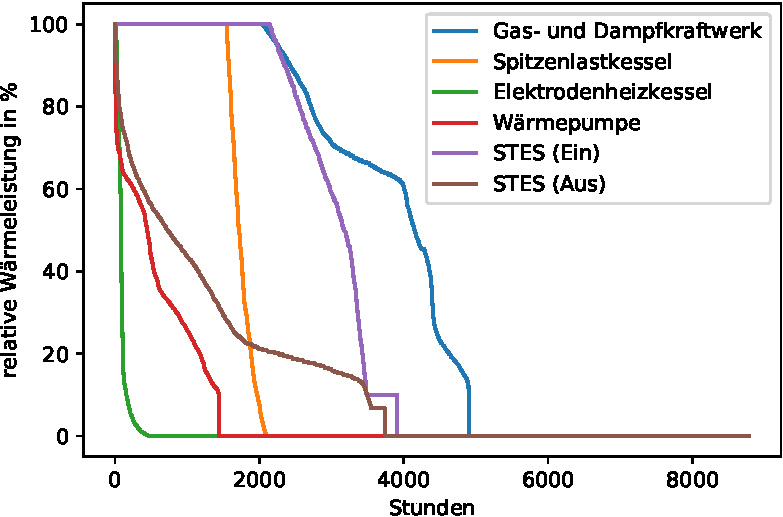
\includegraphics[width=0.8\textwidth]{Jahresdauerlinie_Photovoltaik-cropped.pdf}
		\captionof{figure}[Jahresdauerlinien Photovoltaik]{Illustration des Anlagenbetriebs innerhalb des Photovoltaik-Konzepts als Jahresdauerlinien. Es ist die relative Wärmeleistung der Anlage über den Betriebsstunden bei einer Modulfläche von 70.000~m² und einer Speicherkapazität von 20~GWh dargestellt.}
		\label{figure: Jahresdauerlinie_Photovoltaik}
	\end{figure}

Es stellt sich nunmehr die Frage, welchen Anteil der durch die \ac{PV}-Anlage bereitgestellte Strom zum Betrieb der Wärmepumpe - wie es in diesem Konzept vorgesehen ist - genutzt wurde. Zu diesem Zweck ist der \ac{PV}-Ertrag mit der elektrischen Leistung der Wärmepumpen verglichen worden. Sofern der Bedarf der \ac{WP} den Ertrag der \ac{PV}-Anlage überschreitet, ist angenommen worden, dass 100\% des \ac{PV}-Stroms zum Betrieb der \ac{WP} genutzt wurde. Übersteigt die elektrische Leistung der \ac{PV}-Anlage den Bedarf der \ac{WP}, ist angenommen worden, dass diese komplett durch \ac{PV} betrieben wird. 

Es zeigt sich, dass 33,53\% des \ac{PV}-Stroms zur Wärmebereitstellung durch die Wärmepumpen genutzt wird - 66,47\% werden am Spotmarkt vermarktet. Über die jeweiligen Leistungszahlen kann die entsprechende Wärmeproduktion - allein durch \ac{PV} - auf 9348,26~MWh berechnet werden. Dies entspricht 1,43\% an der gesamten Wärmeproduktion (ca. 1/3 im Vergleich zur Solarthermie) und nimmt somit eine eher untergeordnete Rolle bei der Wärmeversorgung ein. Abbildung \ref{figure: Verhalten_PV} soll das Verhalten der Wärmepumpe weiter veranschaulichen. Dargestellt wird der Ertrag der \ac{PV}-Module über dem von den Wärmepumpen in Summe abgegebenen Wärmestrom $\dot{Q}_{\textit{WP}}$ und dem Strompreis für den 11.06. und 12.06.2016. Es ist deutlich zu erkennen, dass auch mit hohem \ac{PV}-Ertrag die Wärmepumpe ausschließlich bei niedrigen Strompreisen betrieben wird - andernfalls ist es wirtschaftlicher, den Strom am Spotmarkt zu vermarkten. Darüber hinaus ist zu erkennen, dass bei entsprechend hohem \ac{PV} Dargebot die \ac{WP} ausschließlich über die \ac{PV}-Anlage betrieben wird. Dies ist an 248 Stunden des Jahres der Fall.
	\begin{figure}[ht]
		\centering
		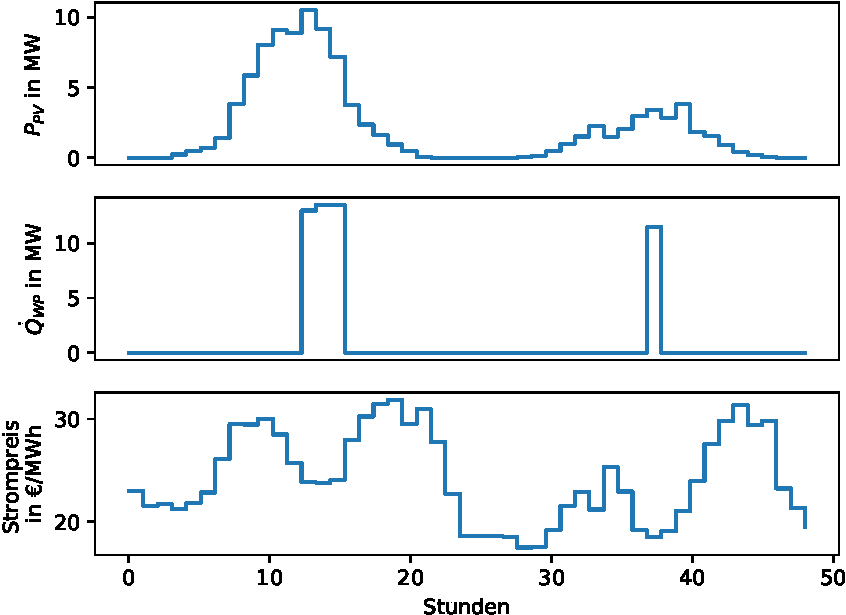
\includegraphics[width=0.8\textwidth]{Photovoltaik_Verhalten_11_06-cropped.pdf}
		\captionof{figure}[Illustration des PV- und Wärmepumpen-Ertrags über dem Strompreis]{Illustration des PV-Ertrags $P_{PV}$, dem von den Wärmepumpen in Summe abgegebenen Wärmestrom $\dot{Q}_{WP}$ über dem Strompreis für den 11.06. und 12.06.2016}
		\label{figure: Verhalten_PV}
	\end{figure}

Auf eine Darstellung des saisonalen Wärmespeichers wird an dieser Stelle verzichtet. Der Ladezustand des Speichers hat einen ähnlichen Verlauf wie der Speicher im ST1-Konzept. Zwischen August und Oktober wird der Speicher innerhalb dieses Konzepts auf einen höheren Stand geladen - ansonsten gleichen sich die Verläufe jedoch stark. Eine Abbildung des über das Jahr aufgetragenen Ladezustands kann dem Anhang (\ref{Anhang: Ladezustand}) entnommen werden.

\subsubsection*{Einflussanalyse des Photovoltaik-Konzepts}
Bereits in der Einflussanalyse zum ST1-Konzept ist der Einfluss des saisonalen Speichers untersucht worden. Es hat sich gezeigt, dass der saisonale Speicher den Einsatz der Anlagen, durch die Entkopplung von Erzeugung und Bedarf, erheblich verbessert. Für die Wärmepumpe in der Einflussanalyse zum ST2-Konzept konnte dargelegt werden, dass diese an sich den Betrieb nur minimal verbessert - in diesem Fall bestand jedoch nicht die Möglichkeit die Wärmepumpe regenerativ über den Strom einer \ac{PV}-Anlage zu betreiben. Aus diesem Grund wird an dieser Stelle die Auswirkung der \ac{PV}-Anlage und der Wärmepumpen auf das Betriebsergebnis des \ac{PV}-Konzepts untersucht.

Zunächst ist das PV-Konzept ausschließlich mit den \ac{PV}-Modulen optimiert worden. In diesem Fall besteht nur die Möglichkeit \ac{PV}-Strom über den \ac{EHK} in Wärme umzuwandeln. Dies wird bei sehr niedrigen Strompreisen auch getan - die Betriebsstunden des \ac{EHK} haben sich von 479~h auf 851~h erhöht und somit fast verdoppelt. Die Tatsache, dass der Erlös des Systems ohne Wärmepumpen über dem Erlös des normalen \ac{PV}-Konzepts liegt ist darüber zu erklären, dass die Optimierung mit einer Genauigkeit von 1\% durchgeführt worden ist. Daraus kann gefolgert werden, dass durch zusätzlich installierte Wärmepumpen, wie bereits beim ST2-Konzept, das Betriebsergebnis -~bei den zugrunde gelegten Randbedingungen~- nur geringfügig verbessert werden kann. Höhere Investitionskosten der \ac{WP} sorgen jedoch dafür, dass der Kapitalwert deutlich abnimmt. Tabelle \ref{tabelle: Übersicht Einflussanalyse PV} fasst die Ergebnisse aller Einflussanalysen zusammen. Die Ergebnisse der ursprünglich untersuchten Konzepte sind in der Tabelle hervorgehoben.
	\begin{center}
		\captionof{table}{Übersicht über die Ergebnisse aller Einflussanalysen} 
		\label{tabelle: Übersicht Einflussanalyse PV}
		\begin{tabular}{lcccc}
			\hline 
			&  & Erlös M\euro/a & Kapitalwert M\euro & \ac{LCOH} \euro/MWh\tabularnewline
			
			\hline 
			\textbf{Solarthermie 1 (normal)}  &  & \textbf{48,13} & \textbf{19,50} & \textbf{30,08} \tabularnewline
			nur mit \ac{STES}		 &  & 47,68 & 33,16 & 28,26 \tabularnewline
			nur mit Solarthermie 	 &  & 44,48 & -17,71 & 35,08 \tabularnewline
			\textbf{Solarthermie 2 (normal)}  &  & \textbf{48,17} & \textbf{13,53} & \textbf{30,88} \tabularnewline
			nur mit \ac{WP}			 &  & 48,00 & 11,83 & 31,11\tabularnewline
			nur mit \ac{STTES} 		 &  & 48,08 & 18,63 & 30,19\tabularnewline
			ST1 mit doppelter Beladung 		 &  & 48,31 & 21,95 & 29,76\tabularnewline
			\textbf{Photovoltaik (normal) }   &  &\textbf{47,99} & \textbf{13,46} & \textbf{30,9} \tabularnewline
			nur mit \ac{PV} 		 &  & 48,09 & 27,13 & 29,07\tabularnewline
			nur mit \ac{WP}			 &  & 47,67 & 20,53 & 29,95\tabularnewline
			\hline
		\end{tabular}
	\end{center} 
\chapter{Diskussion der Ergebnisse}\label{chapter: Diskussion der Ergebnisse}
\thispagestyle{empty}
Folgendes Kapitel wird die Ergebnisse dieser Arbeit zusammenfassen und eine Einschätzung über die Belastbarkeit der Resultate geben. Zunächst wird im ersten Abschnitt dargelegt, welche Schlussfolgerungen dieser Arbeit zu entnehmen sind. Dafür werden die Ergebnisse der Einsatzoptimierung noch einmal vergleichend gegenübergestellt. Daran anschließend folgt eine kritische Betrachtung dieser Arbeit, in der die Belastbarkeit der erzielten Ergebnisse besprochen wird. Abschließend ist in einem Ausblick dargestellt, was im Rahmen dieser Arbeit nicht berücksichtigt ist und stellt somit mögliche Ansatzpunkte für anschließende Arbeiten hervor.

\section{Schlussfolgerungen}\label{section: Schlussfolgerungen}
Die vorliegende Arbeit untersucht die Einsatzmöglichkeiten drei unterschiedlicher solarthermischer Konzepte zur Wärmeversorgung in einem bestehenden Versorgungssystem für den norddeutschen Raum. Zur Bewertung der drei Solarthermie-Konzepte ist zunächst ein Referenzsystem, bestehend aus einer \ac{KWK}-Anlage, einem \acl{SLK} und \acl{EHK}, erstellt worden, welches um die zu untersuchenden Konzepte erweitert wird. Bei dem ersten Solarthermie-Konzept handelt es sich um die Erweiterung des Systems um ein Kollektorfeld und einen saisonalen Wärmespeicher. Das zweite Konzept bindet zusätzlich eine Wärmepumpe und einen Kurzzeitspeicher in das System ein - so soll eine Wärmeversorgung mit erhöhtem \ac{P2H}-Anteil betrachtet werden. Das letzte Konzept untersucht ein System, bei dem die Wärme über eine Kombination aus einer \ac{PV}-Anlage und Wärmepumpen bereitgestellt wird. Bei allen Konzepten werden jeweils drei unterschiedliche Auslegungen für die Kollektorfläche und Speicherkapazität betrachtet. Zur Bestimmung eines ökonomisch optimalen Ergebnisses wird die gemischt-ganzzahlige Optimierung verwendet. Der so ermittelte Erlös des Systems wird, zusammen mit den Investitionskosten, genutzt, um für alle Varianten einen Kapitalwert zu ermitteln.

Es zeigt sich, dass prinzipiell alle betrachteten Konzepte und Szenarien den Kapitalwert des Referenzsystems erhöhen. Gleichzeitig hat der Vergleich aller Kapitalwerte offenbart, dass bei den solarthermischen Konzepten eine Erhöhung der Kollektorfläche und des Speichervolumens zu negativen Kapitalwerten führt. Das betrachtete System aus \ac{PV} und Wärmepumpen weist mit zunehmender Dimensionierung ebenfalls eine Abnahme des Kapitalwerts auf. Im Gegensatz zu den Solarthermie-Systemen nimmt der Kapitalwert des \ac{PV}-Systems jedoch keinen negativen Wert an und stellt somit bei jeder betrachteten Auslegung eine Verbesserung des Referenzsystems dar. Es lässt sich festhalten, dass von den betrachteten Szenarien, jene mit der geringsten Kollektorfläche und Speicherkapazität am wirtschaftlichsten sind. Der Vergleich aller Szenarien zeigt darüber hinaus, dass das einfache Solarthermie-Konzept unter den betrachteten Konzepten den höchsten Kapitalwert erreicht und somit - unter den verwendeten Randbedingungen -  das zu empfehlende Konzept darstellt. 

Das \ac{PV}-Konzept weist wegen der Investitionskosten für die Wärmepumpen - trotz eines höheren Erlöses und niedrigerer Kosten der \ac{PV}-Module - einen geringeren Kapitalwert als das entsprechende Solarthermie-Konzept auf. Die von der \ac{PV}-Anlage bereitgestellte elektrische Energie wird zu 33,5\% für den Betrieb der Wärmepumpe eingesetzt und stellt somit 1,43\% der gesamten Wärmeproduktion, was wiederum ca. 1/3 der Solarthermie entspricht, bereit. Es lässt sich folgern, dass der \ac{PV}-Strom bevorzugt direkt vermarktet wird und nur bei einem geringen Strompreis zur Wärmeproduktion Verwendung findet.

Eine anschließende Einflussanalyse, die den Einfluss einzelner Technologien innerhalb der Konzepte auf das Ergebnis der Optimierung untersucht, zeigt, dass allein die Verwendung eines saisonalen Wärmespeichers den Erlös und Kapitalwert des Systems deutlich erhöht. Die zusätzliche Verwendung einer solarthermischen Anlage steigert den Erlös - sorgt auf Grund der zusätzlichen Investitionskosten jedoch für eine Abnahme des Kapitalwertes. Darüber hinaus hat die Einflussanalyse gezeigt, dass bei Verwendung einer Solarthermie-Anlage ohne Wärmespeicher die Solarthermie nicht gänzlich verwendet werden kann. 

Schließlich kann festgehalten werden, dass durch den Einsatz solarthermischer Wärme - ob direkt durch Solarthermie-Kollektoren oder indirekt durch eine Kombination aus \acl{PV} und Wärmepumpe - das Referenzsystem wirtschaftlicher betrieben werden kann. Das einfache Solarthermie-Konzept stellt dabei unter den untersuchten Konzepten und den zugrunde gelegten Rahmenbedingungen das wirtschaftlich attraktivste Konzept dar. Ein Hinzufügen eines Wärmespeichers ohne Solarthermie hat jedoch die höchste Kapitalwertsteigerung bewirkt - was auf den besseren Betrieb der KWK-Anlage zurückzuführen ist.

\section{Kritische Betrachtung}
Die lineare Optimierung erfordert eine vereinfachte Abbildung aller am Energiesystem beteiligten Komponenten. Im Rahmen dieser Arbeit sind, vor allem aus zeitlichen Gründen, einige Komponenten stärker vereinfacht als andere. Bei der Solarthermie hat die Modellierung ergeben, dass der Ertrag im Preprocessing bestimmt werden kann. Insofern muss die Solarthermie-Anlage nicht linearisiert werden. Mit der GenericCHP-Komponente und dem OffsetTransformer sind zur Abbildung des \ac{GuD} und der \ac{WP} zwei Komponenten gewählt worden, welche die Optimierung zu einem \ac{MILP}-Problem machen, aber eine möglichst genaue Abbildung der Komponenten erlauben. Für den \ac{SLK} und \ac{EHK} ist eine einfachere Modellierung mit einem konstanten Wirkungsgrad gewählt worden, was vor der Erkenntnis, dass der \ac{EHK} kaum und der \ac{SLK} überwiegend bei Nennlast genutzt wird, kaum einen Einfluss auf das Betriebsergebnis hat. Anders verhält es sich bei der Speichermodellierung.

Die verwendeten Wärmespeicher sind, wie der \ac{EHK} und \ac{SLK}, mit einem konstanten Wirkungsgrad auf den austretenden Wärmestrom abgebildet worden. Der Einfluss der Vorlauftemperatur auf das Speicherverhalten oder die Speichertemperatur zur Bestimmung der thermischen Verluste werden in dieser Arbeit nicht berücksichtigt. Über ein Jahr könnten Situationen eintreten, in denen die Speichertemperatur die Vorlauftemperatur des Netzes übersteigt. In diesem Fall kann der Speicher ausschließlich entladen werden. Dies kann mit der vorliegenden Modellierung nicht abgebildet werden.

Darüber hinaus wird in dieser Einsatzoptimierung exemplarisch ein einzelnes Jahr, 2016, betrachtet. Die von dem Betrachtungszeitraum abhängige Einstrahlung und Umgebungstemperaturen haben jedoch einen erheblichen Einfluss auf das Ergebnis der Solarthermie-Anlage sowie \ac{PV}-Anlage und haben somit einen Einfluss auf das Gesamtergebnis der Simulation. Dementsprechend ist bei der Bewertung der Ergebnisse zu berücksichtigen, dass die Umgebungsbedingungen von Jahr zu Jahr variieren und somit das Ergebnis der Einsatzoptimierung bei anderen Betrachtungszeiträumen entsprechend besser oder schlechter ausfallen kann.

Ähnlich verhält es sich bei den angenommenen Kosten für den Strom- und Gasbezug. Diese sind als historische Daten in die Modellierung eingegangen. Es ist jedoch zu bedenken, dass sich diese, wie die Einstrahlung, je nach Betrachtungszeitraum unterscheiden können. Gleiches gilt für die Höhe der Stromabgaben und den CO$_2$-Zertifikatspreis. Im Gegensatz zum realen Betrieb eines Energiesystems, bei dem nur mit kurzfristigen Prognosen gearbeitet werden kann, sind bei der durchgeführten Einsatzoptimierung alle Preiszeitreihen, Wetterdaten und Heizlasten für den gesamten Betrachtungszeitraum bekannt. Die erzielten Ergebnisse der durchgeführten Einsatzoptimierungen sind daher generell als zu hoch einzuschätzen.

\section{Ausblick}
Wie aus Abbildung \ref{fig: Heatmaps Solarthermie} und \ref{figure: Heatmap Photovoltaik} hervorgeht, ist aus wirtschaftlicher Sicht eine Tendenz zu kleineren Anlagendimensionierungen für die Kollektoren und den saisonalen Wärmespeicher zu erkennen. Eine Möglichkeit an diese Arbeit anzuknüpfen ist es daher parallel zur Einsatzoptimierung eine Auslegungsoptimierung der Kollektoren und des Speichers durchzuführen. So kann ein tatsächlich optimales Ergebnis der Einsatzoptimierung erzielt werden. 

Darüber hinaus sind in der vorliegenden Arbeit Solarthermie-Konzepte betrachtet worden, bei denen die Solarthermie direkt in das Wärmeversorgungssystem einspeist. Wie in Kapitel \ref{section: Konzepte} jedoch dargestellt wurde gibt es verschiedene Konzepte, die durch den Einsatz von Wärmepumpen einen Betrieb bei reduzierten Austrittstemperaturen ermöglichen und somit die Effizienz der Solarthermie-Kollektoren erhöhen. Folgende Arbeiten können diese Konzepte untersuchen und klären, ob die zusätzlichen Investitionskosten für die Wärmepumpe eine Effizienzsteigerung der Kollektoren rechtfertigt. 

In diesem Zusammenhang ist es zusätzlich notwendig eine Wasser-Kompressionswärmepumpe abzubilden, die für den Betrieb effizienzsteigender Solarthermie-Konzepte notwendig ist. In dieser Arbeit wird, aus Gründen der zeitlichen Begrenzung, ausschließlich eine Luft-Kompressionswärmepumpe betrachtet. Es ist angenommen worden, dass diese im Winter die Temperaturdifferenz zwischen der Umgebungs- und Vorlauftemperatur zu jedem Zeitpunkt überbrücken kann, dies ist jedoch zu bezweifeln - immerhin kann die Temperaturdifferenz im Winter über 120°C betragen.

Abschließend sollten folgende Arbeiten den Einfluss variierender Energiekosten sowie Investitionskosten untersuchen. Es sollte untersucht werden, welchen Einfluss zunehmende Gas- und CO$_2$-Zertifikatspreise auf die optimale Anlagendimensionierung der Solarthermie-Kollektoren und den Betrieb der \ac{KWK}-Anlage hat, da anzunehmen ist, dass durch zunehmende
Energiekosten höhere Kollektorflächen wirtschaftlich werden.

%\input{src/Fazit}

%Literaturverzeichnis
\newpage
\lhead{}
\rhead{\leftmark}
\addcontentsline{toc}{chapter}{Literaturverzeichnis}
\bibliography{LiteraturDB}

\appendix

\chapter{Anhang}
\thispagestyle{empty}
\section*{Sonnenstandberechnung}\label{Anhang: Sonnenstand}
Die Sonnenstandberechnung (Sonnenhöhe $\gamma_\text{s}$ und Sonnenazimut $\alpha_\text{S}$) ist auf Grundlage des in DIN-5034 \cite{DIN5034} vorgestellten Algorithmus erfolgt. Folgend werden die verwendeten Gleichungen aus \citet{Quaschning2015} dargestellt:

\begin{enumerate}
\item Hilfparameter J' des DIN-Algorithmus:\\
	\begin{equation*}
		J' = 360\text{°} \cdot \dfrac{\text{Tag des Jahres}}{\text{Tage im Jahr}}
	\end{equation*}
\item Sonnendeklination $\delta(J')$ in °
	\begin{equation*}
		\delta(J') = 0,3948 - 23,2559 \cdot \cos(J' - 9,1\text{°}) - 0,3915 \cdot \cos(2J' + 5,4\text{°}) - 0,1764 \cdot \cos(3J'+ 26\text{°})
	\end{equation*}
\item  Zeitgleichung in Minuten
	\begin{equation*}
		Zgl(J') = 0,0066 + 7,3525 \cdot \cos(J' + 85,9\text{°}) + 9,9359 \cdot \cos(2J' + 108,9\text{°}) + 0,3387 \cdot \cos(3J' + 105,2\text{°})
	\end{equation*}
\item Bestimmung der mittleren Ortszeit MOZ in Stunden über die lokale Uhrzeit LZ, die Zeitzone (Stundendifferenz zu UTC-Zeit) und der geographischen Länge $\lambda$
	\begin{equation*}
		\text{MOZ} = \text{LZ} - \text{Zeitzone} + \dfrac{4 \cdot \lambda}{60} 
	\end{equation*}
\item Wahre Ortszeit über Zgl
	\begin{equation*}
		\text{WOZ} = \text{MOZ} - Zgl(J')
	\end{equation*}
\item Stundenwinkel
	\begin{equation*}
		\omega = (12 - \text{WOZ}) \cdot \dfrac{15\text{°}}{\text{h}}
	\end{equation*}
\item[$\Rightarrow$] Sonnenhöhe $\gamma_\text{s}$ über die geographische Breite $\varphi$:
	\begin{equation*}
		\gamma_\text{s} = \arcsin(\cos\omega \cdot \cos\varphi \cdot \cos\delta + \sin\varphi \cdot \sin\delta)
	\end{equation*}
\item[$\Rightarrow$] Sonnenazimut $\alpha_\text{s}$:
	\begin{equation*}
		\alpha_\text{s} = 	\begin{cases}
								180\text{°} - \arccos\dfrac{\sin\gamma_\text{s} \cdot \sin\varphi - \sin\delta}{\cos\gamma_\text{s} \cdot \cos\varphi} & \text{für WOZ $\geq$ 12}\\
								\\
								180\text{°} + \arccos\dfrac{\sin\gamma_\text{s} \cdot \sin\varphi - \sin\delta}{\cos\gamma_\text{s} \cdot \cos\varphi} & \text{für WOZ $<$ 12}
							\end{cases}
	\end{equation*}
\end{enumerate}

\section*{Abbildungen}
	\begin{figure*}[ht]
		\centering
		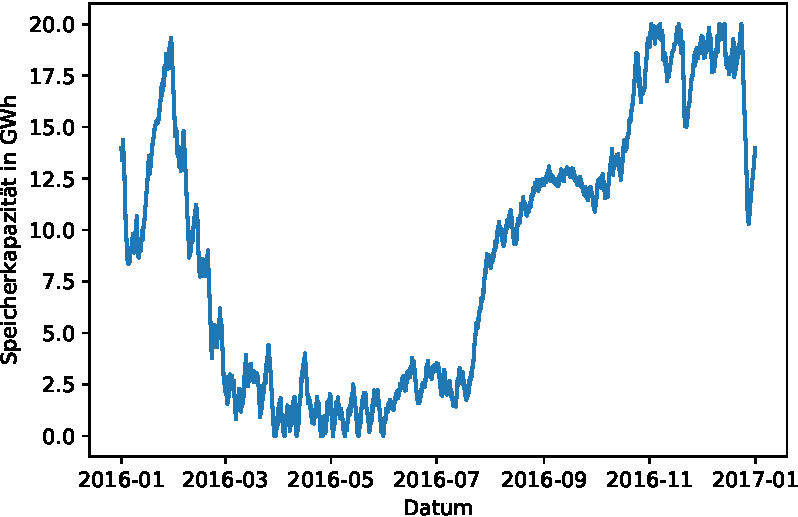
\includegraphics[width=0.8\textwidth]{Speicherverhalten_Photovoltaik-cropped.pdf}
		\captionof{figure}{Darstellung des Ladezustands des saisonalen Wärmespeichers innerhalb des Photovoltaik-Konzepts}
		\label{Anhang: Ladezustand}
	\end{figure*}



\end{document}
